\documentclass[a4paper]{report}
\renewcommand{\baselinestretch}{1.5} 

%% Language and font encodings
\usepackage[utf8]{inputenc}
\usepackage[T1]{fontenc}
\usepackage[square,sort&compress, sectionbib]{natbib}    
% \usepackage[]{natbib}
% \usepackage{chapterbib} 
\usepackage{booktabs}
\usepackage[french,english]{babel}
%% Sets page size and margins
\usepackage[top=1in,left=1.5in,bottom=1in,right=1in]{geometry}

\usepackage{relsize}
%% Useful packages
\usepackage{amsmath, amssymb}
\usepackage{graphicx}
\usepackage{subfig}

\usepackage[
	bookmarks       = true,             % Show the bookmarks
	unicode         = true,             % Use Unicode                 
	pdftoolbar      = true,             % Show Acrobat’s toolbar
	pdfmenubar      = true,             % Show Acrobat’s menu
	pdffitwindow    = false,            % Window fit to page when opened
	pdfstartview    = {FitH},           % Fit the page width to the window
	pdfnewwindow    = true,             % Open the links in a new PDF window
	colorlinks      = true,             % Use colored links
	linkcolor       = blue,             % Internal links color
	citecolor       = blue,            % Bibliographic links color
	filecolor       = cyan,             % File links color
	urlcolor        = magenta           % External links color
]{hyperref}
\usepackage{algorithm}
\usepackage{chapterbib}
\usepackage{algorithmicx}
\usepackage{listings}
\usepackage{algcompatible}
\usepackage{algpseudocode}
\usepackage{tikz}
\usepackage{calc}
\usepackage{pgfplots}
\usepackage{pdfpages}
\pgfplotsset{compat=1.14}
\usepackage{tikzducks}
\usetikzlibrary{snakes}
\usetikzlibrary{positioning}
\usetikzlibrary{shapes,arrows}
\usetikzlibrary{automata,arrows,positioning,calc}

\usetikzlibrary{matrix}
% \usepackage{cmbright}

\makeatletter
\newcounter{algorithmicH}% New algorithmic-like hyperref counter
\let\oldalgorithmic\algorithmic
\renewcommand{\algorithmic}{%
  \stepcounter{algorithmicH}% Step counter
  \oldalgorithmic}% Do what was always done with algorithmic environment
\renewcommand{\theHALG@line}{ALG@line.\thealgorithmicH.\arabic{ALG@line}}
\makeatother

% \geometry{inner=1cm, outer=1cm, top=1cm, bottom=0cm}
\newcommand\fillin[1]{\makebox[#1]{\dotfill}}
% Use a modern font (that is not pixelated)
\usepackage{kpfonts}
% Use microtype to improve readability
\usepackage[protrusion = true, expansion = true]{microtype} 
% Use multiple columns
\usepackage{multicol}
% \usepackage{subfigure}
% \usepackage[subfigure]{tocloft}
% Display list of Equations
% \usepackage{tocloft}
% Insert empty pages
% \usepackage{afterpage}
% Configure style aspects of the document
\usepackage{caption}            % To configure the captions
\usepackage{siunitx}            % For SI units
\usepackage{graphicx}           % To include graphics
% \usepackage[dvipsnames]{xcolor} % To configure colors
\usepackage{fancyhdr}           % To configure the header and footer
% \pagestyle{fancy}               % Use a fancy header style
% \fancyhf{}                      % Set the header format
% \fancyheadoffset{0.0 cm}        % Set the header offset
\lhead{\tfm}                    % Set the header right-side contents
\rhead{\name}                   % Set the header left-side contents
% \cfoot{\thepage}                % Set the footer page number
\usepackage{amsthm}
\usepackage[capitalise,nameinlink,noabbrev]{cleveref}
\crefname{equation}{}{}
\crefname{enumi}{}{}


\newtheorem{lemma}{Lemma}
\newtheorem{theo}{Theorem}
\newtheorem{coro}{Corollary}
\newtheorem{prop}{Proposition}
\newtheorem{property}{Property}
\newtheorem{remark}{Remark}
\newtheorem{ex}{Example}
\newtheorem{exercise}{Exercise}
\newtheorem{definition}{Definition}
\newtheorem{hp}{Assumption}

% Distributions.
\newcommand*{\UnifDist}{\mathsf{Unif}}
\newcommand*{\ExpDist}{\mathsf{Exp}}
\newcommand*{\DepExpDist}{\mathsf{DepExp}}
\newcommand*{\GammaDist}{\mathsf{Gamma}}
\newcommand*{\LognormalDist}{\mathsf{LogNorm}}
\newcommand*{\WeibullDist}{\mathsf{Weib}}
\newcommand*{\ParetoDist}{\mathsf{Par}}
\newcommand*{\NormalDist}{\mathsf{Normal}}

\newcommand*{\GeometricDist}{\mathsf{Geom}}
\newcommand*{\NegBinomialDist}{\mathsf{NegBin}}
\newcommand*{\BinomialDist}{\mathsf{Bin}}
\newcommand*{\PoissonDist}{\mathsf{Poisson}}
\newcommand*{\Cov}{\mathsf{Cov}}

% Sets of numbers.
\newcommand*{\RL}{\mathbb{R}}
\newcommand*{\Z}{\mathbb{Z}}
\newcommand*{\N}{\mathbb{N}}
\newcommand*{\NZ}{\mathbb{N}_0}
% \newcommand*{\NL}{\mathbb{N}_+}

\newcommand*{\cond}{\mid}
\newcommand*{\given}{\,;\,}

%Probability symbols
\newcommand*{\Prob}{\mathbb{P}}
\newcommand*{\Q}{\mathbb{Q}}
\newcommand*{\V}{\mathbb{V}}
\newcommand*{\E}{\mathbb{E}}
\newcommand*{\F}{\mathcal{F}}
\newcommand*{\di}{\text{d}}
% Regarding spacing and abbreviations.
\usepackage{xspace}

% Acronyms
% \@\xspace doesn't add space if next char is punctuation
% However, these will give 2 .'s if used at end of sentence.
\newcommand*{\eg}{e.g.\@\xspace}
\newcommand*{\ps}{p.s.\@\xspace}
\newcommand*{\ie}{i.e.\@\xspace}
\newcommand*{\va}{v.a.\@\xspace}
\newcommand*{\iid}{i.i.d.\@\xspace}
\newcommand*{\ssi}{s.s.i.\@\xspace}
\newcommand*{\cf}{c.f.\@\xspace}
\newcommand*{\pdf}{p.d.f.\@\xspace}
\newcommand*{\pmf}{p.m.f.\@\xspace}
\newcommand*{\cdf}{c.d.f.\@\xspace}
\newcommand*{\SMC}{\textbf{SMC}\@\xspace}
\newcommand*{\MCMC}{\textbf{MCMC}\@\xspace}
\newcommand*{\VF}{\textbf{VF}\@\xspace}


\newcommand*{\iidSim}{\overset{\mathrm{i.i.d.}}{\sim}}
\newcommand*{\bt}{\bm{\theta}}
\newcommand*{\bTheta}{\bm{\Theta}}
\newcommand*{\bbeta}{\bm{\beta}}
\newcommand*{\bx}{\mathbf{x}}
\newcommand*{\bs}{\bm{s}}
\newcommand*{\bu}{\bm{u}}
\newcommand*{\bn}{\bm{n}}

% Roman versions of things.
\newcommand*{\dd}{\mathop{}\!\mathrm{d}}
\newcommand*{\e}{\mathrm{e}}
\DeclareMathOperator*{\argmax}{arg\,max}
\DeclareMathOperator*{\argmin}{arg\,min}

\newcommand*{\norm}[1]{\lVert{} #1\rVert}

% \DeclarePairedDelimiterXPP{\ind}[1]{\ind_}{\{}{\}}{}{#1}
\newcommand*{\ind}{\mathbb{I}}
% \addto\captionsfrench{\def\tablename{{Tableau}}}
\makeatletter

\makeatother
\begin{document}
% \frontmatter
\title{Calcul Stochastique appliqué\\
[0.2em]\smaller{}M1 DUAS - Université de Strasbourg}
\author{Pierre-O Goffard}

\date{updated on \today} 
\maketitle
\tableofcontents
% !TEX root = ../main_lecture_notes.tex
\chapter{Marche aléatoire et Martingale à temps discret}\label{chap:marche_aléatoire}
Ce cours propose une introduction au calcul stochastique avec pour application principale la modèlisation des marchés financiers et la gestion des risque en assurance. L'objet d'étude principale sont les processus stochastiques. 
\begin{definition}\label{def:filtration}
Soit $(\Omega, \F, \Prob)$ un espace probabilisé. Une suite $(X_t)_{t\geq0}$ de variable aléatoires (\va) sur $\Omega$ est un processus stochastique.
  \begin{itemize}
    \item Si $n\in \N$ alors $(X_n)_{n\geq0}$ est un processus stochastique à temps discret. Par exemple une chaine de Markov. 
    \item si $t\in \RL_+$ alors $(X_t)_{t\geq0}$ est un processus stochastique à temps continu. Par exemple le processus de Poisson. 
  \end{itemize}
\end{definition}
% L'utilisation des processus stochastiques pour comprendre le comportements des actifs financiers date des travaux de Bachelier. Près de 70 ans plus tard, Samuelson (prix nobel d'économie en 1970) proposa l'utilisation du mouvement Brownien avec drift. La théorie moderne repose sur les modèles de Black, Scholes and Merton, ce qu'on appelle la théorie des options et les arguments d'absence d'opportunité d'arbitrage. 
% \section{La marche aléatoire et le problème de la double dépense}
% \subsection{Blockchain, cryptomonnaie et double dépense}
% Une blockchain est une base de données constituée de blocs successifs maintenue par un réseau pair-à-pair, comme sur la \cref{fig:blockchain_network}. 
% \begin{figure}[ht!]
% \begin{center}
% \begin{tikzpicture}[-, >=, auto, semithick, node distance=01cm]
% \tikzstyle{every edge}=[segment length=1mm,segment angle=10, draw]

% \tikzstyle{full node}=[circle, fill=blue,draw=blue,thick,text=black,scale=0.8]
% \tikzstyle{light node}=[circle, fill=white,draw=blue,thick,text=black,scale=0.8]
% \node[full node]    (1)                     {};
% \node[full node]    (2)[above right of=1]         {};
% \node[full node]    (3)[above left of=1]         {};
% \node[full node]    (4)[below of=1]         {};
% \node[full node]    (5)[right of=4]         {};
% \node[full node]    (6)[below of=4]         {};
% \node[light node]    (7)[left of=1]         {};
% \node[light node]    (8)[right of=2]         {};
% \node[light node]    (9)[left of=4]         {};
% \node[light node]    (10)[above right of=5]         {};
% \node[light node]    (11)[ right of=5]         {};
% \node[light node]    (12)[ below right of=5]         {};
% % \node[light node]    (4)[above of=2]         {};
% \path

% (1) edge node{} (2)
%     edge node{} (3)
%     edge node{} (7)
%     ;
% \path
% (5) edge node{} (10)
%     edge node{} (11)
%     edge node{} (12)
%     ;
%     \path
% (4) edge node{} (5)
%     edge node{} (1)
%     edge node{} (9)
%     edge node{} (6)
%     ;
%     \path
% (2) edge node{} (8)   
%     ;
% \end{tikzpicture}
% \end{center}
% \caption{Un réseau fait de noeuds lourds (bleu) et de noeuds légers (blanc)}
% \label{fig:blockchain_network}
% \end{figure}
% Les noeuds légers se contentent d'émettre des informations (appelées transactions). Les noeuds lourds doivent vérifier la cohérence des transactions et s'accorder sur les informations à inscrire dans la blockchain. Les noeuds lourds appliquent un protocole de consensus pour se mettre d'accord. La preuve de travail ou \textit{Proof-of-Work} est le protocole utilisé dans le cadre de la blockchain des bitcoins, voir le whitepaper de \citet{Nakamoto2008}. Un bloc doit être ajouté toutes les dix minutes environ, les noeuds sont en compétition pour résoudre un problème cryptographique brutalement via une méthode essai-erreur (\textit{trial and error}). Le premier qui parvient à résoudre le problème ajoute le bloc et récupère une récompense d'un montant de BTC$6.25$ à l'heure de l'écriture.\footnote{\url{https://bitcoinblockhalf.com/}}. \\

% Dans la blockchain des bitcoins, les informations enregistrées sont des échanges de bitcoin entre les participants. Un noeud peut facilement émettre deux transactions conflictuelles, c'est à dire qui transfèrent les mêmes unités à deux entités différentes. Il s'agit d'une attaque par double dépense. Le scénario standard est le suivant:
% \begin{enumerate}
%     \item Marie transfère à John BTC$10$
%     \item La transaction de Marie à John est enregistrée dans la blockchain
%     \item John doit atendre $\alpha\in\N$ confirmations, c'est à dire que $\alpha$ blocs soient ajoutés après celui dans lequel la transaction de Marie à John est inscrite
%     \item Une fois que $\alpha$ confirmations ont été envoyées, John envoie le bien à Marie
%     \item Pendant ce temps, Marie travaille sur sa propre version de la blockchain (dite privée) dans laquelle la transaction de Marie à John est remplacée par une transaction de Marie à elle même
%     \item Au moment de la livraison du bien la blockchain dite principale est en avance de $z$ blocs 
%     \item L'objectif de Marie est générer une chaine concurrente plus longue que la chaine principale. Si elle y parvient, elle la communiquera à l'ensemble du réseau pour créer une fourche (\textit{fork}). Le réseau optera alors pour la branche la plus longue.
%     La branche de Marie va alors remplacer la branche principale permettant à Marie de récupérer ses unités qu'elle peut dépenser à nouveau. 
% \end{enumerate}
% Cette course entre les deux branches est résumée sur la \cref{fig:dp_illustration}.
% \begin{figure}[ht!]
% \begin{center}
% \begin{tikzpicture}[-, >=stealth', auto, semithick, node distance=1cm]
% % \tikzstyle{block} = [rectangle, draw, fill=blue!20,
% %     text width=5em, text centered, rounded corners]
% \tikzstyle{block}=[rectangle, fill=black,draw=black,thick,text=black,scale=1.5]
% \tikzstyle{block}=[rectangle, fill=white,draw=black,thick,text=black,scale=1.5]
% \tikzstyle{confirmed block}=[rectangle, fill=white,draw=blue,thick,text=black,scale=1.5]
% \tikzstyle{bad block}=[rectangle, fill=white,draw=red,thick,text=black,scale=1.5]
% \node[block]    (1)                     {\tiny $\text{M}\rightarrow \text{J}$};
% \node[block]    (2)[right of=1]                     {};
% \node[block]    (3)[right of=2]                     {};
% \node[block]    (4)[right of=3]                     {};
% \node[confirmed block]    (5)[right of=4]                     {};

% \node[bad block]    (6)[below of=1]         {\tiny $\text{M}\rightarrow \text{M}$};
% \node[block]    (7)[right of=6]         {};
% \node[block]    (8)[right of=7]         {};
% \path
% (1) edge[ left]     node{}     (2)
% (2) edge[ left]     node{}     (3)
% (3) edge[ left]     node{}     (4)
% (4) edge[ left]     node{}     (5)
% (6) edge[ left]     node{}     (7)
% (7) edge[ left]     node{}     (8);

% \end{tikzpicture}
% \end{center}
% \caption{La course à la double dépense illustrée, ici nous avons $\alpha = 4$ et $z = 2$}
% \label{fig:dp_illustration}
% \end{figure}
% Notre objectif est de caluler la probabilité que la branche de Marie devienne majoritaire. Pour ce faire nous allons construire un modèle mathématique.
\section{Le problème de ruine du parieur}
Un joueur entre dans un casino pour jouer à la roulette. Nous supposons que notre parieur dispose de $x\in \mathbb{N}$  jetons. Pour faire une partie, le joueur mise $1$ jetons. Il gagne $1$ jetons (et récupère sa mise) avec une probabilité $p\in(0,1)$ et perd sa mise avec probabilité $q = 1-p$.
\subsection{La marche aléatoire sur $\Z$}
Soit $(Z_n)_{n\in\mathbb{N}}$ le nombre de jetons de notre parieur après $n$ parties. On a $Z_0 = z\geq 0$. A chaque instant $k\in\N$ une partie est jouée, 
\begin{itemize}
    \item la partie est gagnée avec probabilité $p\in(0,1)$ et la réserve de jeton augment de $1$
    \item la partie est perdue avec probabilité $q = 1-p$ et la réserve diminue de $1$
\end{itemize}
Soit $(\Omega,\F, \Prob)$ un espace probabilisé. On définit une suite $(\xi_n)_{n\geq0}$ \iid de variables aléatoires (\va) de loi 
$$
\mathbb{P}(\xi = 1) = p\text{, et }\mathbb{P}(\xi = -1) = 1-p.
$$
On en déduit que 
$$
Z_n = z +\sum_{k=1}^n\xi_k.
$$ 
Le processus $Z_n$ est un processus à temps discret et à valeur dans $\Z$ appelé marche ou promenade aléatoire. Le parieur décide de s'arrêter de jouer si sa réserve de jetons atteint le niveau $a$ ou s'il est à cours de jeton. On définit les instants aléatoires
\begin{equation}\label{eq:dp_time}
\tau_0 = \inf\{n\geq0\text{ ; }Z_n = 0\},\text{ et }\tau_a = \inf\{n\geq0\text{ ; }Z_n = a\}.
\end{equation}
Nous souhaitons calculer la probabilité que le parieur rentre chez lui ruiné, c'est à dire 
\begin{equation}\label{eq:ruin_proba}
\phi(z, a) = \Prob(\tau_0 <\tau_a| Z_0 = z).
\end{equation}
Une visualisation du problème de première excursion est donné sur la \cref{fig:ruin_time}.
\begin{figure}[ht!]
\begin{center}
\begin{tikzpicture}
  %Origin and axis
  \coordinate (O) at (0,0);
  \draw[->] (-1,0) -- (9,0) coordinate[label = {below:$n$}] (xmax);
  \draw[->] (0,-0.5) -- (0,3) coordinate[label = {left:$Z_n$}] (ymax);
  \draw[dashed, -] (0,2.5) -- (9,2.5) coordinate[] (xmax);
  %Lower linear boundary

 
  %Stochastic process trajectory
  
  \draw (0,0) node[blue,left] {} node{};
  \draw[very thick,blue,-] (0,1) -- (1,1) node[pos=0.5, above] {} ;
  \draw[very thick,dashed,blue] (1,1) -- (1,1.5) node[pos=0.5, right] {};
  \draw[very thick,blue,-] (1,1.5) -- (2,1.5) node[pos=0.5, above] {};
  \draw[very thick,dashed,blue] (2,1.5) -- (2,2) node[pos=0.5, right] {};
  \draw[very thick,blue,-] (2,2) -- (3,2) node[pos=0.5, above] {};
  \draw[very thick,dashed,blue] (3,2) -- (3,1.5) node[pos=0.5, right] {};
  \draw[very thick,blue,-] (3,1.5) -- (4,1.5)node[pos=0.5, above] {};
  \draw[very thick,dashed,blue] (4,1.5) -- (4,1) node[pos=0.5, right] {};  
  \draw[very thick,blue,-] (4,1) -- (5,1) node[pos=0.5, above] {};
  \draw[very thick,dashed,blue] (5,1) -- (5,0.5) node[pos=0.5, right] {};  
  \draw[very thick,blue,-] (5,0.5) -- (6,0.5) node[pos=0.5, above] {};
  \draw[very thick,dashed,blue,-] (6,0.5) -- (6,1) node[pos=0.5, above] {};
   \draw[very thick,blue,-] (6,1) -- (7,1) node[pos=0.5, above] {};
    \draw[very thick,dashed,blue,-] (7,1) -- (7,0.5) node[pos=0.5, above] {};
     \draw[very thick,blue,-] (7,0.5) -- (8,0.5) node[pos=0.5, above] {};
     \draw[very thick,dashed,blue,-] (8,0.5) -- (8,0) node[pos=0.5, above] {};
  %Jump Times
  \draw (1,0) node[black,below] {$1$} node{ \color{black}$\bullet$};
  \draw (2,0) node[black,below] {$2$} node{ \color{black}$\bullet$};
  \draw (3,0) node[black,below] {$3$} node{ \color{black}$\bullet$};
  \draw (4,0) node[black,below] {$4$} node{ \color{black}$\bullet$};
  \draw (5,0) node[black,below] {$5$} node{ \color{black}$\bullet$};
  \draw (6,0) node[black,below] {$6$} node{ \color{black}$\bullet$};
  \draw (7,0) node[black,below] {$7$} node{ \color{black}$\bullet$};
  \draw (8,0) node[black,below] {$8$} node{ \color{black}$\bullet$};
  %Level of the counting process
   \draw (0,0) node[black,below left] {$0$} node{ \color{black}$\bullet$};
   \draw (0,0.5) node[black,left] {$1$} node{ \color{black}$\bullet$};
   \draw (0,1) node[black,left] {$z=2$} node{ \color{black}$\bullet$};
   \draw (0,1.5) node[black,left] {$3$} node{ \color{black}$\bullet$};
   \draw (0,2) node[black,left] {$4$} node{ \color{black}$\bullet$};
   \draw (0,2.5) node[black,left] {$a=5$} node{ \color{black}$\bullet$};

  % %Aggregated Capital gains
%  \draw (0,1.5) node[blue,below right] {$\mu_1$} node{ \color{blue}$-$};
%  \draw (0,2.25) node[blue,left] {$\mu_2$} node{ \color{blue}$-$};
%  \draw (0,3.75) node[blue,left] {$\mu_3$} node{ \color{blue}$-$};
  %Ruin time = First-crossing time time
%  \draw (5,0) node[black,above right] {${\tau_0}_u$} node{ \color{black}$\times$};
%  \draw[dotted,black] (0,3.28) -- (5,3.28);
%  \draw[dotted,black] (5,0) -- (5,3.28);
\end{tikzpicture}
\end{center}
\caption{Illustration du problème de premier passage sous-jacent à la double dépense.}
\label{fig:ruin_time}
\end{figure}

Le processus $Z$ est une chaine de Markov.
\subsection{Filtration, chaine de Markov et temps d'arrêt}
Soit $(\Omega,\F, \Prob)$ un espace probabilisé sur lequel on définit un processus $X:=(X_n)_{n\geq0}$. 
\begin{definition}\label{def:filtration}
Une filtration $(\F_n)_{n\geq0}$ est une suite de sous-tribu de $\F$, croissante pour l'inclusion au sens où
$$
\F_k\subset \F_n,\text{ pour }k\leq n.
$$

\end{definition}
$\F_n$ correspond à l'information disponible au temps $n$. C'est aussi l'information nécessaire pour tracer la trajectoire du processus jusqu'à l'instant $n$.
\begin{definition}\label{def:processus_adapte}
Le processus X est $\F_n$-adapté si $X_n$ est mesurable par rapport $\F_n$. La suite
$$
\F_n = \sigma(X_1,\ldots, X_n),\text{ }n\in \N,
$$ 
est la filtration naturelle du processus $X$.
\end{definition}
\begin{ex}\label{ex:filtration_marche_aleatoire}
La marche aléatoire $Z_n$ est adaptée à la filtration $$
\F_n = \sigma(\xi_k,\text{ }k\leq n).
$$
\end{ex}
Soit un processus $X:=(X_n)_{n\geq0}$ adapté à la filtration $(\F_n)_{n\geq0}$ à valeur dans l'espace d'état $E$.
\begin{definition}\label{def:CM}
Le processus $X$ sur un espace d'état $E$ vérifie la propriété de Markov simple si pour toute fonction mesurable $g:E\mapsto \RL$,
$$
\E[g(X_{n+1})|\F_{n}] = \E[g(X_{n+1})|X_{n}].
$$

 
 \end{definition}
\begin{ex}
Un processus $X$ sur un espace d'état $E$ est une chaine de Markov s'il vérifie la propriété suivante
$$
\mathbb{P}(X_{n+1} = x_{n+1}|X_{n}=x_{n},\ldots, X_0 = x_0) = \mathbb{P}(X_n = x_n|X_{n-1}=x_{n-1}), \text{ pour tout }(x_0,\ldots, x_{n+1})\in E^{n+2}.
$$

Les chaines de Markov vérifie la propriété de Markov simple, en prenant $g = \mathbb{I}_{y}(\cdot)$ pour $y\in E$. Le processus $X$ est une chaine de Markov homogène (CMH) si
$$
\mathbb{P}(X_{n+1} = x|X_{n}=x) = \mathbb{P}(X_{1} = x|X_{0}=x)\text{ pour tout }n\in\mathbb{N}\text{ et }(x,y)\in E^2.
$$
Une CMH est caractérisée par son espace d'état, sa loi initiale 
$$
\mu(x) = \Prob(X_0 = x),
$$
et ses probabilités de transitions notées
$$
p(x,y) = \Prob(X_{n+1} = y|X_{n}= x),\text{ pour tout }n\geq0\text{ et }(x,y)\in E^2.
$$
% En effet, on a 
% \begin{eqnarray*}
% \Prob(X_0 = x_0, \ldots, X_{n-1} = x_{n-1}, X_n = x_n) &=& \Prob(X_n = x_n|X_{n-1} = x_{n-1}\ldots, X_{1} = x_{1}, X_0 = x_0)\\
% &\times&\Prob(X_{n-1} = x_{n-1}\ldots, X_{1} = x_{1}, X_0 = x_0)\\
% &=& \Prob(X_n = x_n|X_{n-1} = x_{n-1})\\
% &\times&\Prob(X_{n-1} = x_{n-1}\ldots, X_{1} = x_{1}, X_0 = x_0)\\
% &=& p(x_{n-1},x_n)P(X_{n-1} = x_{n-1}\ldots, X_{1} = x_{1}, X_0 = x_0)\\
% &\vdots&\\
% &=&\Prob(X_0= x_0)p(x_0,x_1)\ldots p(x_{n-1}, x_n)\\
% &=&\mu(x_0)p(x_0,x_1)\ldots p(x_{n-1}, x_n).
% \end{eqnarray*}
Lorsque l'espace d'état $E$ est fini, la loi initiale et les probabilités de transition forment respectivement est un vecteur et une matrice indicés sur $E$ avec
$$
\mu = (\mu(x))_{x\in E},\text{ et }P = (p(x,y))_{(x,y)\in E}.
$$
% Les calculs de probabilités se résument alors à des calculs matriciels. La loi de $X_n$ sachant que $X_0\sim \mu$ est donnée par 
% $\mu\cdot P^n$.
% La somme des coefficients sur chaque ligne de $P$ doit être égale à $1$, car 
% $$
% \sum_{y\in E}p(x,y) = \sum_{y\in E}\Prob(X_{n+1} = y|X_n = x) = 1,\text{ pour tout }n\in\mathbb{N}\text{ et }x\in E.
% $$
\end{ex}



\begin{prop}
Soit $(X_n)_{n\in\N}$ une chaine de Markov homogène de loi initiale $\mu$ et de matrice de transition $\mathbf{P}$. On a
$$
\Prob(X_0 = x_0,X_1 = x_1,\ldots, X_n = x_n) = \mu(x_0)p(x_0,x_1)\ldots p(x_{n-1},x_n).
$$
En particulier, on a (sous réserve que $\Prob(X_0 = x_0)>0$),
$$
\Prob(X_n = x_n|X_0 = x_0) = P^{n}(x_0, x_n),
$$
où $P^{n}(x_0, x_n)$ est le terme générale de la matrice $P^{n}$, et
$$
\Prob(X_n = x_n) =  \boldsymbol{\mu} P^{n}(\text{ . } , x_n),
$$
où $\boldsymbol{\mu}$ est un vecteur ligne donnant les probabilités de la loi initiale et $P^{n}(\text{ . } , x_n)$ est le vecteur colonne de la matrice $P^{n}$ donnant les probabilité de transition vers l'état $x_n$.
\end{prop}
\begin{proof}
On conditionne en cascade avec
\begin{eqnarray*}
\Prob(X_0 = x_0, \ldots, X_{n-1} = x_{n-1}, X_n = x_n) &=& \Prob(X_n = x_n|X_{n-1} = x_{n-1}\ldots, X_{1} = x_{1}, X_0 = x_0)\\
&\times&\Prob(X_{n-1} = x_{n-1}\ldots, X_{1} = x_{1}, X_0 = x_0)\\
&=& \Prob(X_n = x_n|X_{n-1} = x_{n-1})\\
&\times&\Prob(X_{n-1} = x_{n-1}\ldots, X_{1} = x_{1}, X_0 = x_0)\\
&=& p(x_{n-1},x_n)P(X_{n-1} = x_{n-1}\ldots, X_{1} = x_{1}, X_0 = x_0)\\
&\vdots&\\
&=&\Prob(X_0= x_0)p(x_0,x_1)\ldots p(x_{n-1}, x_n)\\
&=&\mu(x_0)p(x_0,x_1)\ldots p(x_{n-1}, x_n).
\end{eqnarray*}
En ce qui concerne la seconde assertion, on conditionne par rapport à tout les chemins possibles menant de $x_0$ à $x_n$ en $n$ étapes,
\begin{eqnarray*}
\Prob(X_n = x_n|X_0 = x_0) &=& \sum_{(x_1,\ldots, x_{n-1})\in E^{n-1}}\Prob(X_n = x_n, X_{n-1} = x_{n-1},\ldots, X_1 = x_1|X_0 = x_0) \\
&=& \sum_{(x_1,\ldots, x_{n-1})\in E^{n-1}}p(x_0,x_1)\ldots p(x_{n-1}, x_n)\\
&=&P^{n}(x_0,x_n).
\end{eqnarray*}
Pour la dernière assertion, on conditionne par rapport aux valeurs possibles de l'état initial
\begin{eqnarray*}
\Prob(X_n = x_n) &=& \sum_{x_0\in E}\Prob(X_n = x_n|X_0 = x_0)\Prob(X_0 = x_0)\\
&=& \sum_{x_0\in E}\mu(x_0)P^n(x_0,x_n)\\
&=& \boldsymbol{\mu}P^n(\text{ . },x_n)
\end{eqnarray*}
\end{proof}
\begin{prop}
Soit $(\xi_n)_{n\geq1}$ une suite de \va \iid et indépendante de la \va $X_0$ à valeur dans $G$. Le processus
$$
X_n = F(X_{n-1}, \xi_n),\text{ }n\geq1,
$$
pour toute fonction mesurable $F:E\times G\mapsto E$ est une CMH.
\end{prop}
\begin{proof}
Soit $n\in\mathbb{N}$ et $x_0,\ldots,x_{n+1}\in E$. Posons $A_n=\{X_0=x_0,\ldots,X_n=x_n\}$, alors on a
\begin{eqnarray*}
\mathbb{P}(X_{n+1}=x_{n+1}|A_n)&=&\mathbb{P}[F(X_n,\xi_{n+1}))=x_{n+1}|A_n]\\
&=&\mathbb{P}[F(x_n,\xi_{n+1}))=x_{n+1}|A_n]\\
&=&\mathbb{P}[F(x_n,\xi_{n+1}))=x_{n+1}]\\
&=&\mathbb{P}[F(x_n,\xi))=x_{n+1}].\\
\end{eqnarray*}
Le processus $(X_n)_{n\in\mathbb{N}}$ est une chaine de Markov homogène de matrice de transition
$$
p(x,y)=\mathbb{P}(F(x,\xi)=y),\text{ }\forall (x,y)\in E^{2}.
$$
\end{proof}
\begin{ex}
On observe que la marche aléatoire $Z$ vérifie
$$
Z_{n} = Z_{n-1} + \xi_{n},\text{ }n\geq1.
$$
Il s'agit bien d'une CMH dont les probabilités de transitions sont données par 
$$
p(x,y) = \begin{cases}
p&\text{ si }y = x+1,\\
1-p&\text{ si }y = x-1,\\
0& \text{ sinon}.
\end{cases}
$$
\end{ex}
\begin{definition}\label{def:temps_arret}
Une variable aléatoire $\tau:\Omega\mapsto \overline{\mathbb{N}}_+ = \mathbb{N}_+\cup\{+\infty\}$ est un temps d'arrêt pour le processus $X$ et sa filtration $(\F_n)_{n\geq0}$ si 
$$
\{\tau\leq n\}\in \F_n\text{, pour tout }n\geq1.
$$
\end{definition}
\begin{ex}\label{ex:dp_time}
Le temps de ruine $\tau_0 = \inf\{n \geq0\text{ ; }Z_n = 0\}$ est un temps d'arrêt du processus $Z$. En effet, on peut écrire 
$$
\{\tau_0=n \} = \bigcap_{k=1}^{n-1}\{Z_k\neq 0\}\cap\{Z_n = 0\}.
$$
\end{ex}

\begin{definition}\label{def:markov_forte}
Un processus $X$ vérifie la propriété de Markov forte si pour $\tau$ un temps d'arrêt et $g:E\mapsto \RL$ mesurable, on a 
$$
\E[g(X_{\tau + n})|\F_\tau]= \E[g(X_{\tau + n})|X_\tau].
$$
\end{definition}
Une CMH $X$ vérifie la propriété de Markov forte. En fait, pour temps d'arrêt fini presque surement, la chaine de Markov $\tilde{X}=(X_{n+\tau})_{n\geq0}$ a les mêmes caractéristiques que $X$. C'est à dire même espace d'état et probabilités de transition, seule la loi initiale diffère avec
$$
\tilde{\mu}(x) = \Prob(\tilde{X}_0 = x) = \Prob(X_\tau = x).
$$ 
La propriété de Markov forte permet l'étude de temps tel que $\tau_0$. L'application de cette propriété au temps $\tau = 1$ (les constantes sont des temps d'arrêt) est l'analyse à un pas qui permet notamment de démontrer le résultat suivant:
% L'étude des temps d'arrêt comme $\tau_0$ procède de l'analyse à un pas décrite dans le résultat suivant.  Soit $\Prob_x(\cdot)$ et $\E_x(\cdot)$ la probabilité et l'espérance conditionnelle sachant $X_0 = x$. 
% \begin{prop}
% Soit $\tau_A=\inf\{n\geq0\text{ ; }X_n\in A\}$, avec $A\subset E$ tel que $\E_x(\tau_A)<\infty$ pour tout $x\in E$. Soit $x\in E$ et $n\geq1$, alors
% \begin{enumerate}
% \item
% $$
% \Prob_x(\tau_A=n)=
% \begin{cases}
% 0,&\text{ }x\in A,\\
% \sum_{y\in E}p(x,y)\Prob_y(\tau_A=n-1),&x\notin A.
% \end{cases}
% $$
% \item
% $$
% \E_x(\tau_A)=
% \begin{cases}
% 0,&\text{ }x\in A,\\
% 1+\sum_{y\in E}p(x,y)\E_y(\tau_A),&x\notin A.
% \end{cases}
% $$
% \end{enumerate}
% \end{prop}
% \begin{proof}
% \begin{enumerate}
%     \item Si $x\in A$ alors $\tau_A = 0$ $\Prob_x$-p.s. donc
%     $\Prob_x(\tau_A=n)=0\text{ pour }n\geq1\text{ et }\Prob_x(\tau_A=0)=1$.
%     Supposons $n = 1$ alors
%     \begin{eqnarray*}
%         \Prob_x(\tau_A=1)&=&\Prob(\tau_A=1|X_0=x)\\
%         &=&\sum_{y\in E} \Prob(\tau_A=1, X_1=y|X_0=x)\\
%         &=&\sum_{y\in A} \Prob(\tau_A=1 |X_1=y,X_0=x)p(x,y) \\
%         &+& \sum_{y\in E/A} \Prob(\tau_A=1|X_1=y,X_0=x)p(x,y)\\
%         &=&\sum_{y\in A} 1\times  p(x,y) + 0.\\
%     \end{eqnarray*}
%     On remplace $1$ par $\Prob_y(\tau_A=0)$ (=1 si $y\in A$), il vient
%     $$
%     \Prob_x(\tau_A=1)= \sum_{y\in A} \Prob_y(\tau_A=0)\times  p(x,y)
%     $$
%     quite à ajouter $0$ on a
%     \begin{eqnarray*}
%     \Prob_x(\tau_A=1)&=& \sum_{y\in A} \Prob_y(\tau_A=0)\times  p(x,y) + 0\\
%      &=&\sum_{y\in A} \Prob_y(\tau_A=0)\times  p(x,y)\\
%      &+& \sum_{y\in E/A} \Prob_y(\tau_A=0)\times  p(x,y).
%     \end{eqnarray*}
%     puisque $\Prob_y(\tau_A=0) = 0$ si $y\in E/A$. On vérifie bien que
%     $$
%     \Prob_x(\tau_A=n)=\sum_{y\in E}p(x,y)\Prob_y(\tau_A=n-1)\text{ pour }n = 1.
%     $$
%     Supposons $n>1$ alors
%     \begin{eqnarray*}
%     \Prob_x(\tau_A=n)&=&\Prob(\tau_A=n|X_0=x)\\
%     &=&\sum_{y\in E} \Prob(\tau_A=n, X_1=y|X_0=x)\\
%     &=&\sum_{y\in A} \Prob(\tau_A=n |X_1=y,X_0=x)p(x,y) \\
%     &+& \sum_{y\in E/A} \Prob(\tau_A=n|X_1=y,X_0=x)p(x,y)\\
%     &=& 0+ \sum_{y\in E/A} \Prob(\tau_A=n|X_1=y,X_0=x)p(x,y)\\
%     &=&  \sum_{y\in E/A} \Prob\left(\bigcap_{i = 0}^{n-1}\{X_i\notin A\}\cap\{X_n\in A\}|X_1=y,X_0=x\right)p(x,y)\\
%     \end{eqnarray*}
%     Sachant $\{X_0 = x\}$ l'évènement $\{X_0 \notin A\}$ est presque sûr. On a donc
%      $$
%      \Prob_x(\tau_A=n)=  \sum_{y\in E/A} \Prob\left(\bigcap_{i = 1}^{n-1}\{X_i\notin A\}\cap\{X_n\in A\}|X_1=y\right)p(x,y)
%      $$
%      On perd le conditionnement par rapport à $X_0$ car sachant $X_1$
%      $$
%      \bigcap_{i = 1}^{n-1}\{X_i\notin A\}\cap\{X_n\in A\}\text{ est indépendant de } X_0.
%      $$
%      Puis on remarque que comme $(X_n)_n\in \N$ est une CMH alors
%      $$
%      [(X_1, X_2,\ldots, X_n)|X_1  =y]\overset{\mathcal{D}}{=}[(X_0, X_1,\ldots, X_{n-1})|X_0 = y].
%      $$
%      Cela permet d'écrire
%     \begin{eqnarray*}
%     \Prob_x(\tau_A=n)&=&\sum_{y\in E/A} \Prob_y\left(\bigcap_{i = 0}^{n-2}\{X_i\notin A\}\cap\{X_{n-1}\in A\}\right)p(x,y)\\
%     &=&\sum_{y\in E/A} \Prob_y\left(\tau_A = n-1\right)p(x,y) + 0\\
%     &=&\sum_{y\in E} \Prob_y\left(\tau_A = n-1\right)p(x,y).
%     \end{eqnarray*}
%     \item Si $x\in A$ alors $\E_x(\tau_A)=0$ et sinon
% \begin{eqnarray*}
% \E_x(\tau_A)&=&\sum_{n=0}^{+\infty}n\times\Prob_x(\tau_A=n)\\
% &=&\sum_{n=1}^{+\infty}n\sum_{y\in E}\Prob_y(\tau_A=n-1)p(x,y)\\
% &=&\sum_{y\in E}p(x,y)\sum_{n=0}^{\infty}(n+1)\Prob_y(\tau_A=n)\\
% &=&\sum_{y\in E}p(x,y)(1+ \E_y(\tau_A))\\
% &=&1+\sum_{y\in E}p(x,y)\E_y(\tau_A).
% \end{eqnarray*}

% \end{enumerate}
% \end{proof}
\begin{theo}\label{theo_ruin_proba}
\begin{equation}\label{eq:gambler_ruin}
\phi(z,a) = \begin{cases}
\frac{(q/p)^z-(q/p)^a}{1 - (q/p)^a}&\text{ if }p\neq q,\\
\frac{a-z}{a}&\text{ if }p= q.
\end{cases}
\end{equation}
\end{theo}
\begin{proof}
Par la loi des probabilités totales, on a
\begin{equation}\label{eq:difference_equation}
\phi(z,a) = p\phi(z+1,a)+(1-p)\phi(z-1,a),\text{ }z\geq1.
\end{equation}
Nous avons également les conditions lmites suivantes
\begin{equation}\label{eq:boundary_conditions_double_spending}
\phi(0,a) = 1\text{ and }\phi(a,a) = 0.
\end{equation}
L'équation \eqref{eq:difference_equation} définie une suite récurrente linéaire d'ordre 2\footnote{Pour rappel \url{https://www.bibmath.net/formulaire/index.php?action=affiche&quoi=suitereclin}.} associé à l'équation caractéristique
\begin{equation}\label{eq:characteristic_equation}
px^2 - x + 1-p = 0.
\end{equation}
\begin{enumerate}

\item Supposons que $p=1-p=1/2$ alors \eqref{eq:characteristic_equation} a une unique solution $r = 1$. Les suites définies par \eqref{eq:difference_equation} sont données par
$$
\phi(z,a) = A+Bz.
$$
L'utilisation des conditions limites \eqref{eq:boundary_conditions_double_spending} conduit à
$$
\phi(z,a) = \frac{a-z}{a},
$$
comme annoncé.
\item Supposons que $p\neq q = 1-p$ alors \eqref{eq:characteristic_equation} a deux solutions réelles
$$
r_1 = 1, \text{ and }r_2 = \frac{1-p}{p}.
$$
Les suites définies par \eqref{eq:difference_equation} sont de la forme
$$
\phi(z,a)=A+B\left(\frac{1-p}{p}\right)^z,
$$
où $A$ et $B$ sont des constantes. Les conditions limites \eqref{eq:boundary_conditions_double_spending}, implique que
$$
\phi(z,a) = \frac{(q/p)^z-(q/p)^a}{1 - (q/p)^a},
$$
comme annoncé.
\end{enumerate}
\end{proof}

\begin{remark}
Sur le comportement asymptotique de $Z$ en fonction de la valeur de $p$. On a par la loi des grands nombres
$$
\frac{Z_n}{n}=\frac{Z_0}{n}+\frac{1}{n}\sum_{k=1}^{n}\xi_k\underset{n\rightarrow+\infty}{\longrightarrow} 2p-1.
$$
On en déduit que
$$
Z_n\rightarrow\begin{cases}
-\infty,&\text{ si }p<1/2,\\
? (0\times \infty),&\text{ si }p=1/2,\\
+\infty,&\text{ si }p>1/2.\\
\end{cases}
$$
Dans le cas $p=1/2$ le processus oscille. Par le théorème centrale limite, on observe que pour $n$ très grand $Z_n\sim\NormalDist(z, \sqrt{n})$. Le \cref{theo_ruin_proba} avec $a\rightarrow \infty$ nous indique que 
\begin{equation}\label{eq:ds_proba}
\phi(z, \infty) = \Prob(\tau_0 < \infty)=\begin{cases}
1,\text{ si }p\leq 1/2,\\
(q/p)^z,\text{ si } p> \frac 12.
\end{cases}
\end{equation}
Dans le cas $p=1/2$, on montre que l'état $0$ est récurrent. Cette notion est abordée en annexe, voir l'annexe \ref{app:convergence_martingale}. le résultat \eqref{eq:ds_proba} est prouvé en td et une application à l'étude du problème de la double dépense dans le contexte d'une blockchain est évoqué dans l'annexe \ref{app:application_blockchain}
\end{remark}
Il est aussi possible de donner la loi de probabilité de $\tau_0$ via le résultat suivant.
\begin{theo}
Si $z = 0$ alors $\tau_0=0$ \ps. Si $z>0$ alors la loi de $\tau_0$ est donnée par
$$
\mathbb{P}_z(\tau_0 = n)=
\frac{z}{n}\binom{n}{(n-z) / 2}p^{(n-z) / 2}(1-p)^{(n
+z) / 2}\text{ si }n\geq z\text{ et }n-z\text{ est pair},
$$
et $0$ sinon.
\end{theo}
\begin{proof}
Nous avons besoin du lemme suivant.
\begin{lemma}\label{lem:markov_hitting_time}
\begin{equation}\label{eq:markov_hitting_time}
\mathbb{P}_z(\tau_0 = n) = \frac{z}{n}\mathbb{P}_z(Z_n = 0).
\end{equation}
\end{lemma}
\begin{proof}
Si $z = 0$ alors $\tau_0 = 0$ \ps et les deux membres \eqref{eq:markov_hitting_time} sont égaux à $0$. Supposons que $z\geq1$, nous avons $\mathbb{P}_z(\tau_0 = n) = 0$ et $\mathbb{P}_z(Z_n = 0) = 0$ lorsque $n<z$ et $n-z$ est impair. On raisonne par récurrence sur $n\geq1$, quand $n = 1$ nous avons
$$
\mathbb{P}_z(\tau_0 = 1) = 0 = \frac{z}{1}\mathbb{P}_z(Z_1 = 0),\text{ pour }z>1, 
$$
et 
$$\mathbb{P}_1(\tau_0 = 1) = q = \frac{1}{1}\mathbb{P}_1(Z_1 = 0),\text{ pour }z=1. 
$$
La propiété est vérifiée pour $n=1$. Supposons qu'elle soit vérifiée au rang $n>1$. En vertu de la loi des probabilités totales, nous avons 
\begin{eqnarray*}
\mathbb{P}_z(\tau_0 = n+1)&=&\sum_{y\in\{-1,1\}}\mathbb{P}_z(\tau_0 = n+1|\xi_1 = y)\mathbb{P}(\xi_1 = y)\\
&=&\sum_{y\in\{-1,1\}}\mathbb{P}_{z+y}(\tau_0 = n)\mathbb{P}(\xi_1 = y)\\
&=&\sum_{y\in\{-1,1\}}\frac{z+y}{n}\mathbb{P}_{z+y}(Z_n = 0)\mathbb{P}(\xi_1 = y)
\end{eqnarray*}
Pour la deuxième égalité, nous avons eu recours à la propriété de Markov forte. Nous "détricottons" la loi des probabilités totales pour obtenir
\begin{eqnarray}
\mathbb{P}_z(\tau_0 = n+1)&=&\sum_{y\in\{-1,1\}}\frac{z+y}{n}\mathbb{P}_{z+y}(Z_n = 0)\mathbb{P}(\xi_1 = y)\nonumber\\
&=&\sum_{y\in\{-1,1\}}\frac{z+y}{n}\mathbb{P}_{z}(Z_{n+1} = 0|\xi_1 = y)\mathbb{P}(\xi_1 = y)\label{eq:law_total_probability_undone_1}\\
&=&\sum_{y\in\{-1,1\}}\frac{z+y}{n}\mathbb{P}_{z}(\xi_1 = y|Z_{n+1} = 0)\mathbb{P}_z(Z_{n+1} = 0)\nonumber\\
&=&\frac{\mathbb{P}_z(Z_{n+1} = 0)}{n}\left[z+\mathbb{E}_z(\xi_1|Z_{n+1}=0)\right]\label{eq:law_total_probability_undone_2}
\end{eqnarray}
Le passage à \eqref{eq:law_total_probability_undone_1} s'explique par l'égalité suivante: 
$$
[Z_n|Z_0 = z+y] = [Z_{n+1}|Z_0 = z, \xi_1 = y ]\text{ }\mathbb{P}-\text{ p.s.}.
$$
Comme les $\xi_i$ sont \iid alors il vient 
$$
\mathbb{E}_z(\xi_1|Z_{n+1}=0) = \mathbb{E}_z(\xi_i|Z_{n+1}=0)\text{, } i = 1, \ldots, n+1,
$$
et par suite 
$$
\mathbb{E}_z(\xi_1|Z_{n+1}=0) = \frac{1}{n+1}\sum_{i =1}^{n+1}\mathbb{E}_z(\xi_i|Z_{n+1}=0) = \frac{-z}{n+1}.
$$
En injectant l'expression ci-dessus dans \eqref{eq:law_total_probability_undone_2}, il vient 
$$
\mathbb{P}_z(\tau_0 = n+1) = \frac{z}{n+1}\mathbb{P}_z(Z_{n+1} = 0).
$$
\end{proof}
Pour compléter la preuve, on remarque simplement que
$$
\mathbb{P}_z(Z_n = 0) = \binom{n}{(n-z) / 2}p^{(n-z) / 2}q^{(n
+z) / 2}.
$$
Il s'agit de la probabilité d'occurence d'une trajectoire de $(Z_n)_{n \geq0}$ commençant au niveau $Z_0 = z$ finissant au niveau $0$ comprenant $(n-z)/2$ sauts vers le haut et $(n+z)/2$ sauts vers le bas.
\end{proof}

\subsection{Loi invariante, récurrence et loi stationnaire}
Soit $(X_{n})_{n\in\N}$ une chaine de Markov homogène d'espace d'état $E$.
\begin{definition}[Irréductibilité]
La chaine de Markov $(X_n)_{n\in\N}$ est irréductible si pour tout $(x,y)\in E^{2}$, il existe $n\in\N$ tel que
$$P^{n}(x,y)=\mathbb{P}(X_n=y|X_0=x)>0.$$
\end{definition}
\begin{ex}
La marche aléatoire sur $\mathbb{Z}$ est irréductible. En effet, pour $n = |x-y|$, on a 
$$
\mathbb{P}(X_n=y|X_0=x) = \begin{cases}
p^{y-x},&\text{ si } y\geq x,\\
q^{x-y},&\text{ sinon }.\\
\end{cases}
$$
\end{ex}

\begin{definition}[Loi invariante]
Soit $\mu$ une loi de probabilité sur $E$. $\mu$ est une loi invariante si 
$$
\mu(y) = \sum_{x\in E}\mu(x)p(x,y),
$$
soit matriciellement $$\mu = \mu \mathbf{P}.$$
\end{definition}
\begin{definition}[Loi réversible]
Soit $\lambda$ une loi de probabilité sur $E$. $\lambda$ est une mesure reversible si
$$
\lambda(x)p(x,y) = \lambda(y)p(y,x),\text{ pour tout }x,y\in E.
$$
\end{definition}
\begin{prop}
$$
\lambda \text{ reversible }\Rightarrow  \lambda \text{ invariante.}
$$
\end{prop}
\begin{proof}
On a
$$
\sum_{x\in E}\lambda(x)p(x,y)=\sum_{x\in E}\lambda(y)p(y,x) =\lambda(y)
$$
\end{proof}
\begin{ex}[Modèle d'urne d'Erhenfest]
Dans deux urnes $A$ et $B$ se trouvent $N$ boules numérotées de $1$ à $N$. Le processus $(X_n)_{n\in \N}$ correspond au nombre de boules présente dans l'urne $A$. On suppose qu'initialement toutes les boules sont dans l'urne $A$ (soit $X_0 = N$). A chaque pas de temps
\begin{enumerate}
    \item On tire un numéro $i$ au hasard dans $\{1,\ldots, n\}$
    \item La boule portant le numéro $i$ change d'urne
\end{enumerate}
Le processus $(X_n)_{n\in \N}$ est une CMH d'espace d'état $E = \{0,\ldots, N\}$ de probabilité de transition
$$
p(x,y) = \begin{cases}
\frac{N-x}{N},&\text{ si }y = x+1,\text{ et }x = 0,\ldots, N-1, \\
\frac{x}{N},&\text{ si }y = x-1,\text{ et }x = 1,\ldots, N,\\
0&\text{ sinon}.
\end{cases}
$$
Une loi $\lambda$ est réversible si et seulement si elle vérifie
$$
\lambda(x)\frac{N-x}{N} = \lambda(x+1)\frac{x+1}{N},\text{ }x= 0,\ldots, N-1\text{ et }\sum_{x\in E}\lambda(x) = 1.
$$
On remarque alors que $\lambda(x) = \binom{N}{x}2^{-N}$ convient.
\end{ex}
Soit $x\in E$, on notera la probabilité et l'espérance conditionnelle de $X_n$ sachant $X_0=x$ de la façon suivante
$$
\mathbb{P}(X_n=y|X_0=x)=\mathbb{P}_{x}(X_n=y)\text{, }y\in E,\text{ et }\mathbb{E}(X_n|X_0=x)=\mathbb{E}_{x}(X_n).
$$
Soit $X:=(X_n)_{n\in\mathbb{N}}$ une CMH sur $E$. On note

$$
R_x=\inf\{n\geq 1\text{ ; }X_n=x\}
$$ 
le temps de retour à l'état $x$ (en supposant que $X_0=x$).
\begin{definition}[Etat récurrent/transitoire]
Un état $x\in E$ est
\begin{enumerate}
\item récurrent si
$$
\mathbb{P}_x(R_x<\infty)=1,
$$ 
\begin{itemize}
    \item récurrent positif si $\E_x(R_x) <\infty$
    \item récurrent nul si $\E_x(R_x) =\infty$
\end{itemize}
\item est transitoire
$$
\mathbb{P}_x(R_x=\infty)>0
$$
\end{enumerate}
Un état est transitoire lorsqu'il n'est pas récurrent.
\end{definition}
Si $(X_n)_{n\geq 0}$ est une CMH irréductible alors les états sont tous soit récurrents soit transitoires.
% \begin{theo}\label{theo:loi_invariante_existence_unicite}
% Soit $(X_n)_{n\geq 0}$ est une CMH irréductible et récurrente alors
% \begin{enumerate}
%     \item Soit il existe une unique mesure de probabilité invariante $\pi$ et on a pour tout $x\in E$
%     $$
%     \pi(x) = \frac{1}{E_x(R_x)},
%     $$
%     la chaine est dite récurrente positive.
%     \item Soit il n'existe pas de mesure de probabilité (les mesures invariantes ont une masse totale infinie) et pour tout $x\in E$
%     $$
%     \E_x(R_x) = \infty,
%     $$
%     la chaine est dite récurrente nulle. 
% \end{enumerate}
% \end{theo}

\begin{theo}
La marche aléatoire sur $\mathbb{Z}$ est irréductible et
\begin{itemize}
\item Récurrente si $p=1/2$.
\item transitoire sinon.
\end{itemize}
\end{theo}
\begin{proof}
Pour montrer ce résultat, on étudie la distribution du temps $R_0$ de retour à $0$. On a
$$
\mathbb{P}_0(R_0<\infty)=\sum_{n=1}^{+\infty}\mathbb{P}_0(R_0=n).
$$
On remarque que les trajectoires allant de $0$ à $0$ sont nécessairement de longueur paire et
$$
\mathbb{P}_0(R_0=2n+1)=0,\text{ pour } n=0,1,\ldots.
$$
et
$$
\mathbb{P}_0(R_0<\infty)=\sum_{n=1}^{+\infty}\mathbb{P}_0(R_0=2n).
$$
On a exactement $\binom{2n}{n}$ trajectoires possibles, celle qui nous intéresse (pour lesquels $R_0=2n$) sont celles qui ne repassent pas par $0$ entre l'instant $0$ et $2n$ (On parle d'excursions). Leur nombre est donné par
\begin{equation}\label{eq:NombreBonnesTrajectoires}
2\times C_{n-1}=2\times \frac{1}{n}\binom{2n-2}{n-1}
\end{equation}
\begin{definition}[Nombre de Catalan]
Les nombres de Catalan sont définis par
$$
C_n=\frac{1}{n+1}\binom{2n}{n},\text{ pour }n\geq 0,
$$
et vérifie
\begin{equation}\label{eq:RecurrenceDyckWord}
C_{n+1}=\sum_{k=0}^{n}C_kC_{n-k}\text{ pour }n\geq1
\end{equation}
\end{definition}
\begin{ex}[Mots de Dyck]
$C_n$ correspond aux nombre de mots de $2n$ lettres comprenant respectivement $n$ A et $n$ B, tels que lu de gauche à droite le nombre de $A$ demeure supérieur ou égal au nombre de $B$. La relation de récurrence \eqref{eq:RecurrenceDyckWord} s'explique par le fait qu'un mot de Dyck contenant plus de deux lettres est obtenu par la concaténation de deux mots de Dyck.
\end{ex}
Dans le problème considéré, on s'intéresse aux nombres de mots tels que le nombre de $A$ (interprétés comme des $+1$) soit strictement supérieur au nombre de $B$ (interprétés comme des $-1$). Alors notre mot commence nécessairement par un $A$ et fini sur un $B$. La portion entre ce $A$ et ce $B$ est un mot de Dyck contenant $2n-2$ lettres. On a $C_{n-1}$ possibilités. Le facteur $2$ dans \eqref{eq:NombreBonnesTrajectoires} s'explique par la symétrie du problème puisque l'on peut considérer les trajectoires dans lesquels les $-1$ dominent les $+1$. La probabilité d'une trajectoire quelconque de longueur $2n$ contenant $n$ "$+1$" et $n$ "$-1$" est donnée par $p^{n}(1-p)^{n}$, on en déduit que
\begin{eqnarray}
\mathbb{P}_0(R_0<\infty)&=&\sum_{n=1}^{+\infty}\mathbb{P}_0(R_0=n)=\sum_{n=1}^{+\infty}2C_{n-1}[p(1-p)]^{n}\nonumber\\
&=&2p(1-p)\sum_{n=0}^{+\infty}C_{n}[p(1-p)]^{n}=2p(1-p)C[p(1-p)],\label{eq:ProbaS0}
\end{eqnarray}
où $C(x)=\sum_{n=0}^{+\infty}C_nx^{n}$. Or, on a
\begin{eqnarray*}
C(x)&=&1+\sum_{n=1}^{+\infty}C_nx^{n}=1+x\sum_{n=0}^{+\infty}C_{n+1}x^{n}\\
&=&1+x\sum_{n=0}^{+\infty}\sum_{n=0}^{n}C_kC_{n-k}x^{n}=1+x\sum_{n=0}^{+\infty}\sum_{n=k}^{n}C_kC_{n-k}x^{n}\\
&=&1+x\sum_{n=0}^{+\infty}C_k\sum_{n=0}^{n}C_{n}x^{n+k}=1+xC(x)^{2}
\end{eqnarray*}
Par suite, $C(x)=\frac{1-\sqrt{1-4x}}{2x}$. En substituant dans \eqref{eq:ProbaS0}, on obtient
$$
\mathbb{P}_0(R_0<\infty)=1-|1-2p|
$$
On en déduit que si $p\neq 1/2$ alors $\mathbb{P}_0(R_0<\infty)<1$ et la chaine est transitoire sinon $\mathbb{P}_0(R_0<\infty)=1$ et la chaine est récurrente.
\end{proof}
\begin{remark}
La marche aléatoire $Z$ telle que $p=1/2$ est récurrente nulle. On rappelle que 
$$
\Prob(R_0 = 2n) =\frac{1}{n}\binom{2n-2}{n-1}4^{-n}.
$$
Par la formule de Stirling, il vient l'équivalent 
$$
\binom{2n-2}{n-1} = \frac{(2n-2)!}{(n-1)!}\sim \frac{4^{n-1}}{\sqrt{\pi n}}
$$
puis
$$
\Prob(R_0 = 2n)\sim \frac{n^{-3/2}}{\sqrt{2}}\text{ lorsque }n\rightarrow \infty.
$$
On en déduit que 
$$
\E_0(R_0) = \sum_{n =1}^{\infty} 2n\Prob(R_0 = 2n)=\infty,
$$
donc la marche aléatoire est récurrente nulle.
% \item La période de la marche aléatoire sur $\Z$ est égale à $2$. La modification 
% $$
% \widetilde{Z}_n = (Z_n)_+ = \max(Z_n, 0)
% $$
% définit une chaine de Markov irréductible, récurrente positive et apériodique si $p <  1/2$. Il s'agit de la marche aléatoire réfléchie en $0$.
% \end{enumerate}
\end{remark}


% \begin{remark}[Divergence lorsque $p\neq 1/2$]
% Dans le cas d'une chaine de Markov $(Z_n)_{n\in\N}$ sur un espace ordonné et dénombrable (comme $\N$ ou $\mathbb{Z}$), si la chaine est transitoire alors elle diverge vers $\infty$. Par exemple dans le cas de la chaine aléatoire sur $\mathbb{Z}$, on a par la loi des grands nombre
% $$
% \frac{Z_n}{n}=\frac{Z_0}{n}+\frac{1}{n}\sum_{k=1}^{n}\xi_k\underset{n\rightarrow+\infty}{\longrightarrow} 2p-1.
% $$
% On en déduit que
% $$
% Z_n\rightarrow\begin{cases}
% -\infty,&\text{ si }p<1/2,\\
% ? (0\times \infty),&\text{ si }p=1/2,\\
% +\infty,&\text{ si }p>1/2.\\
% \end{cases}
% $$
% Dans le cas $p=1/2$ le processus oscille. Par le théorème centrale limite, on observe que pour $n$ très grand $Z_n\sim\NormalDist(z, \sqrt{n})$.
% \end{remark}
\begin{definition}
La période d'un état $x\in E$ est définie par 
$$
d(x) = \text{pgcd}\{n\geq 1\text{ ; }\Prob(X_n=x|X_0 = x)>0\}.
$$
Si $d(x) = 1$ alors $x$ est apériodique. Si $(X_n)_n\in\mathbb{N}$ est irréductible alors tous les états ont la même période. 
\end{definition}

\begin{theo}
Si $(X_n)_{n\in\N}$ est irréductible, récurrente positive et apériodique alors la chaine se stabilise au sens où
$$
\Prob_x(X_n = y)\underset{n\rightarrow \infty}{\rightarrow} \pi(y),\text{ pour tout }x\in E.
$$
La loi $\pi$ est unique et coincide avec la loi invariante. 
\end{theo}

\begin{remark}
Si l'espace d'état $E$ est fini, et que la chaine $X$ est irréductible, alors tous les états sont récurrents positifs. Il existe une unique mesure invariante qui est aussi la mesure stationnaire. Je vous invite à vérifier cela en python sur l'exemple de l'urne d'Erhenfest. Voir \texttt{ehrenfest.ipynb} sur moodle.
\end{remark}


\section{Une marche aléatoire plus générale et le modèle de ruine à temps discret}\label{sec:ruin_discret}
On peut généraliser le processus $Z$ étudier précédemment. 
\subsection{Définition}\label{ssec:definition}
Soit $X:= (X_n)_{n\geq0}$ le processus défini par 
\begin{equation}\label{eq:marche_aleatoire_generale}
X_0 = x,\text{ et }X_n = X_{n-1}+\xi_n,\text{ }n\geq 1,
\end{equation}
où $(\xi_n)_{n\geq0}$ est une suite de \va \iid sur $\RL$. Le processus $X$ est à temps discret et à valeur dans $\RL$.
\begin{ex}\label{ex:ruine_discret}
Soit une compagnie d'assurance non-vie,
\begin{itemize}
\item detenant un capital initial $x>0$,
\item récupérant $c>0$ sur chaque période d'exercice au titre des primes,
\item indemnisant $U$, variable aléatoire positive, à ses assurés sur chaque période d'exercice.
\end{itemize}
Soit $(X_n)_{n\geq0}$ la valeur de la réserve financière à la fin de chaque période d'exercice. On a
$$
X_0=x\text{ et }X_n=x+c\times n - \sum_{k=1}^{n}U_n,\text{ }n=1,2,3,\ldots
$$
où $U_1,U_2,\ldots$ sont des \va \iid positives distribuées comme $U$. On s'intéresse à la probabilité de ruine avant $T$ définie par
$$
\psi(x,T)=\mathbb{P}_x(X_n<0,\text{ pour un certain }n\leq T).
$$
\begin{itemize}
\item Calibrer $c$ $\Rightarrow$ tarification, typiquement
$$
c=\mathbb{E}(U)(1+\eta),
$$
avec un chargement de sécurité $\eta>0$.
\item Calibrer $x$ $\Rightarrow$ provisionnement. Choisir $x$ grand permet d'éviter une ruine à court terme.
\end{itemize}
On retombe sur le processus \eqref{eq:marche_aleatoire_generale} en prenant 
$$
\xi = c - U.
$$
\end{ex}
Le calcul de la probabilité de ruine s'effectue en utilisant la propriété de Martingale de la marche aléatoire. 
\subsection{Martingale à temps discret}
\begin{definition}
Un processus $(X_n)_{n\geq0}$ est une martingale pour une filtration $\mathcal{F}_n$, si
\begin{itemize}
  \item[(i)] $X_n$ est $\mathcal{F}_n$-adapté,
  \item[(ii)] $\mathbb{E}(|X_n|)<\infty\text{ pour }n\geq0$,
  \item[(iii)] $\mathbb{E}(X_{n+1}|\mathcal{F}_{n}) = X_{n}$.
\end{itemize} 
\end{definition}
\begin{definition}
Le processus $X$ est une sur-martingale (resp. sous-martingale) si
    $$
    \E(X_{n+1}|\mathcal{F}_n) \leq (\text{resp. } \geq ) X_n,\text{ pour tout } n\in \N.
    $$
    On désignera par le terme S-martingale une sous ou sur martingale
\end{definition}
\begin{remark}    
Une sur-martingale décroit en moyenne tandis qu'une sous-martingale croit en moyenne. On note également que si $(X_n)_{n\in \N}$ est une martingale alors
$$
\E(X_m|\F_n) = X_n,\text{ pour tout }0\leq n\leq m.
$$
En effet, on note que 
$$
\E(X_m|\F_n) = \E(\E(X_m|\mathcal{F}_{m-1})|\F_n) = \E(X_{m-1}|\mathcal{F}_n) =\ldots, \E(X_{n}|\mathcal{F}_n) = X_n.
$$
On note également que cela entraine
$$
\E(X_m)=\E(X_n)=\E(X_0).
$$
\end{remark}
\begin{ex}
\begin{enumerate}
    \item Soit $X_1,\ldots, X_n$ une suite de \va \iid  intégrables tels que $\E(X_i) = 0$ pour tout $i\geq 1$ alors leur somme
    $$
    S_n = X_1+\ldots+X_n,\text{ pour tout }n\geq1,
    $$
    définit une martingale par rapport à la filtration $\mathcal{F}_n = \sigma(X_1,\ldots, X_n)$. En effet,
    $$
    \E(|S_n|)\leq \E\left(\sum_{i=1}^n|X_i|\right)\leq n\cdot\E(|X|) <\infty.
    $$
    et
    $$
    \E(S_{n+1}|\F_n) =\E(S_{n}+X_{n+1}|\F_n) = S_n + \E(X_{n+1}) = S_n.
    $$
    
    \item Soit $X_1,\ldots, X_n$ une suite de v.a. positives i.i.d. et intégrables telles que $\E(X_i) = 1$ pour tout $i\geq 1$ alors leur produit
    $$
    M_n = \prod_{i=1}^n X_i,\text{ }n\geq1,
    $$
    définit une martingale par rapport à la filtration $\sigma(X_1,\ldots, X_n)$. En effet,
    $$
\E(|M_n|) = \prod_{i=1}^n\E(|X_i|) = \E(|X|)^n <\infty,
    $$
    et
    $$
    \E(M_{n+1}|\F_n) =\E(X_{n+1}M_n|\F_n) = M_n\E(X_{n+1}) = M_n.
    $$
    \item Soit $\xi$ une v.a. tel que $\E(|\xi|)<\infty$, le processus $M_n = \E(\xi|\F_n),\text{ }n\geq1$ qui correspond à la valeur moyenne de la variable aléatoire $\xi$ étant donnée l'information collectée $\F_n$ jusqu'a l'instant $n\geq1$, définit une martingale. En effet, 
    $$
\E(|M_n|) = \E(|\E(\xi|\mathcal{F}_n)|) \leq \E(|\E(|\xi||\mathcal{F}_n)) = \E(|\xi|),
    $$
    et
    $$
    \E(M_{n+1}|\F_n) = \E(\E(\xi|\F_{n+1})|\F_n) =\E(\xi|\F_n) = M_n.
    $$
    Il s'agit d'une propriété de l'espérance conditionnelle. Pour $Z$ $\mathcal{F}_n$-mesurable et bornée, on a d'une part 
    
    $$
    \E(\E(\xi|\mathcal{F}_{n+1})Z)=\E(\E(Z\xi|\mathcal{F}_{n+1})) = \E(\xi Z)
    $$
    et d'autre part
    $$
    \E(\E(\xi|\mathcal{F}_{n+1})Z)=\E(\E(Z\E(\xi|\mathcal{F}_{n+1})|\mathcal{F}_n)) =  \E(Z\E(\E(\xi|\mathcal{F}_{n+1})|\mathcal{F}_n))
    $$
    On en déduit que $\E(Z\E(\E(\xi|\mathcal{F}_{n+1})|\mathcal{F}_n)) = \E(\xi Z)$ or $E(\xi|\mathcal{F}_{n})$ est la seule \va $\mathcal{F}_n$ mesurable telle que 
    $$
    \E(Z\xi) = \E(Z\E(\xi|\mathcal{F}_n)).
    $$
\end{enumerate}
\end{ex}
\begin{definition}
Un processus $(H_n)_{n\in\N}$ est $\mathcal{F}_n$-prévisible si
$$
H_n\text{ est borné et }\mathcal{F}_{n-1}\text{-mesurable}.
$$
\end{definition}
\begin{prop}\label{prop:ladder_process}
Soit $(X_n)_{n\in\N}$ un processus adapté et $(H_n)_{n\in\N}$ un processus prévisible alors le processus définie par
$$
(H.X)_0 =0\text{, }(H.X)_n =H_1(X_1-X_0)+\ldots+ H_n(X_n-X_{n-1}),\text{ }n\geq1
$$
est une martingale (resp. une surmartingale) si $(X_n)_{n\in\N}$ est une martingale (resp. sur-martingale).
\end{prop}
\begin{proof}
Il faut montrer que
$$
\E\left[(H.X)_{n+1} - (H.X)_{n}|\mathcal{F}_n\right]=0.
$$
On note que
$$
\E\left[(H.X)_{n+1} - (H.X)_{n}|\mathcal{F}_n\right]=\E\left[H_{n+1}(X_{n+1}-X_n)|\mathcal{F}_n\right]=0.
$$
\end{proof}
\begin{remark}
\begin{enumerate}
% \item la construction \cref{prop:ladder_process} a une interpretation en mathématiques financières. Supposons que 
% \begin{itemize}
%     \item $(X_n)_{n\in\mathbb{N}}$ soit la valeur d'un actif financier au cours du temps
%     \item $(H_n)_{n\in\mathbb{N}}$ soit le nombre de parts de cet actif détenue par un investisseur.  
% \end{itemize}
% Alors $H.X$ est la valeur du portefeuille de l'investisseur. 
% \item Lorsque $X$ est une marche aléatoire sur $\Z$, on peut interpréter $H.X$ comme la richesse d'un parieur. A chaque instant $n$, Le parieur joue à un jeu, il gagne avec probabilité $p$ et perd avec probabilité $1-p$. Le processus $(H_n)_{n\geq 1}$ est la somme pariée (sa stratégie). Le cumul des gains (ou perte si négatif) jusqu'au temps $n$ est exactement $(H\cdot Z)_n$. 
\item Le processus $H.X$ est aussi appelée intégrale stochastique discrète et on écrit 
 $$
 (H\cdot X)_n = \sum_{k = 1}^n H_{k}(X_{k}-X_{k-1}) = \int_1^n H_k\text{d}X_k.
 $$
 C'est un outil pratique pour les démonstrations.
\end{enumerate}
\end{remark}
\begin{theo}[du temps d'arrêt optionnel]\label{theo:temps_arret}
Soient $(X_n)_{n\in\N}$ une martingale (rsp. sur-martingale) et $\tau$ un $\mathcal{F}_n$ temps d'arrêt. Le processus $(X_{n\land \tau})_{n\in\N}$ est une martingale (resp. une sur-martingale). De plus, si $\tau$ est bornée alors
$$
\E(X_{\tau}) = \E(X_0).
$$
\end{theo}
\begin{proof}
On remarque que le processus définie par
$$
H_{n} = \mathbb{I}_{\tau\geq n} = 1 -\mathbb{I}_{\tau\leq n-1}
$$
est prévisible et que
$$
(X_{n\land \tau})_{n\in\N} = X_0 + (H.X)_n\text{ (on peut le montrer par récurrence)}
$$
est donc une martingale (si $(X_n)_{n\in\N}$ est une martingale). Comme $\tau$ est bornée alors il existe $N\in\N$ tel que $\tau\leq N$ presque surement. On en déduit que
$$
\E(X_{\tau})=\E(X_{\tau\land N})=\E(X_0).
$$
\end{proof}
\begin{remark}
Lorsqu'on ne sait pas si $\tau$ est borné ou qu'il n'est tout simplement pas bornée. L'astuce consiste à considéré le temps d'arrêt $\tau\land n$ puis à faire tendre $n$ vers l'infini. Cela fonctionne lorsque le processus $X$ tend vers $0$ asymptotiquement. 
\end{remark}

Le résultat précédent s'étend à des temps d'arrêt quelconques sous réserve d'ajouter une hypothèse d'uniforme intégrabilité. On peut aussi démontrer l'existence de limite pour les processus martingales. Ces résultats sont résumés en annexe, voir \cref{app:convergence_martingale}. Pour un exposé exhaustif sur les martingales en temps discret, le lecteur peut se référer aux note de cours de \citet[Chapitre 13]{LeGall2006} \footnote{\url{https://www.imo.universite-paris-saclay.fr/~jean-francois.le-gall/IPPA2.pdf}}, à l'ouvrage de \citet[Chapitre 4]{laleuf14} et pour les anglophones à l'ouvrage de \citet{Williams1991}.

\subsection{Probabilité de ruine dans le modèle de risque à temps discret}
La richesse d'une compagnie d'assurance est modélisée par la marche aléatoire $X$, défini par 
$$
X_0 = x,\text{ }X_n = X_{n-1} +\xi_n,\text{ }n\geq 1, 
$$
où les $\xi$ sont \iid et $\F_n = \sigma(\xi_1,\ldots, \xi_n)$. Nous avons besoin de définir la martingale de Wald. 
\begin{prop}
Le processus  
$$
M_n = \exp(\theta X_n - n\kappa(\theta)),\text{ pour }n\geq1,
$$
pour $\theta\in \RL$ tel que $\kappa(\theta) = \log\E(e^{\theta\xi})<\infty$ est une $\F_n$-martingale.
\end{prop}
\begin{proof}
On a 
\begin{eqnarray*}
\E(|M_{n}|) &=& \E(M_{n})\\
&=& e^{\theta x}<\infty
\end{eqnarray*}
et
\begin{eqnarray*}
\E(M_{n+1}|\F_n) &=& \E[\e^{\theta X_{n+1} - (n+1)\kappa(\theta)}|\F_n]\\
&=& \e^{-(n+1)\kappa(\theta)}\E[\e^{\theta X_{n} +\theta\xi_{n+1} }|\F_n]\\
&=& \e^{-(n+1)\kappa(\theta)}\e^{\theta X_{n}}\E[ \e^{\theta\xi_{n+1} }|\F_n]\\
&=& \e^{-(n+1)\kappa(\theta)}\e^{\theta X_{n}}\E[ \e^{\theta\xi_{n+1} }]\\
&=& \e^{-(n+1)\kappa(\theta)}\e^{\theta X_{n}}\e^{\kappa(\theta)}\\
&=& M_n
\end{eqnarray*}
\end{proof}
Soit 
$$
\tau_0=\inf\{n\geq0\text{ ; }X_n \leq0\} 
$$
On souhaite calculer la probabilité de ruine à horizon de temps infini ($T = \infty$) définie par 
$$
\psi(x) = \psi(x,\infty) = \Prob(\tau_0 <\infty).
$$
Supposons que $\E(\xi)>0$ alors nous avons le résultat suivant 
\begin{prop}
Supposons qu'il existe $\theta^{\ast}>0$ tel que
$$
\log\E(\e^{-\theta\xi}) = 0,
$$
alors
$$
\psi(x) = \psi(x,\infty) = \frac{\e^{-\theta^\ast x}}{\E\left[e^{\theta^\ast d(x)}|\tau_0 <\infty\right]},
$$
où $d(x) = - X_{\tau_0}$ est le déficit à la ruine.
\end{prop}
\begin{proof}
On définit le processus 
$$
Y_n = x - X_n,\text{ }n\geq0.
$$
Il s'agit également d'une marche aléatoire qui démarre à $0$ et dont les sauts sont distribués comme $-\xi$. Le processus 
$$
\e^{\theta Y_n - n\kappa(\theta)},\text{ }n\geq0,
$$
avec $\kappa(\theta) = \log\E(\e^{-\theta\xi})$ est une martingale. Au vu de la définition de $\theta^\ast$, le processus $(\e^{\theta^\ast Y_n})_{n\geq 0}$ est une martingale. Comme $\E(-\xi) <0$ alors $Y_n\rightarrow -\infty$. On remarque que 
$$
\tau_0 = \inf\{n\geq0\text{ ; }X_n\leq0\} = \inf\{n\geq0\text{ ; }Y_n\geq x\}
$$ 
On applique le théorème du temps d'arrêt optionel au temps $\tau_0\land n = \min(\tau_0,n)$ pour $n>0$ au processus $(\e^{\theta^\ast Y_n})_{n\geq 0}$. Il vient 
$$
1 = \E(e^{\theta^{\ast}Y_0}) = \E(e^{\theta^{\ast}Y_{\tau_0\land n}}) = \E(e^{\theta^\ast Y_{\tau_0}}\mathbb{I}_{\tau_0< n} + e^{\theta^\ast Y_n}\mathbb{I}_{\tau_0\geq n})
$$
En laissant $n\rightarrow \infty$, il vient 
$$
\Prob(\tau_0<\infty) = \frac{e^{-\theta^\ast x}}{\E[e^{-\theta^\ast X_{\tau_0}}|\tau_0 <\infty]}.
$$
\end{proof}
\section{Introduction aux mathématiques financières}\label{sec:intro_math_fi}
Le contenu de ce chapitre s'inspire des notes de cours de \citet{Tankov2010}.
% \subsection{Un premier modèle de mathématique financière}
% les actifs financiers sont des produits échangeables sur les marché financiers, ils comprennent 
% \begin{itemize}
%     \item Les actions, titre de propriété partiel d'une entreprise (action d'entreprise du CAC40)
%     \item Les obligations (bond du trésors américain) 
%     \item les commodités (l'or, le pétrole, ...)
% \end{itemize}
% La valeur d'un actif au cours du temps est une suite de variable aléatoire $(S_n)_{n \geq 0}$, indicée sur le temps $n\in\mathbb{N}$.\\ 

% \noindent Un produit dérivé est un actif dont la valeur dépend de la valeur d'un autre actif financier, dit sous-jacent. Les options sont des produits dérivés communs. Les \textit{put} et les \textit{call} permettent l'achat ou la vente d'un titre à un prix fixé à l'avance. 
% \begin{definition}\label{def:eu_option}
% Une Option d'achat (resp. de vente) européenne donne le droit (pas l'obligation) d'acheter un titre à la date $T$ au prix $K$. Le flux de trésorerie (\textit{pay-off}) associé à ce contrat est donnée par 
% $$
% (S_T-K)_{+}\text{ (resp. }(K-S_T)_{+})
% $$ 
% \end{definition}
% \begin{itemize}
% \item Un marché financier permet l'échange d'actif financier et permet également d'emprunter du \textit{cash}. L'emprunt doit être rembourser à un taux d'intérêt $r$ correspondant au rendement d'un actif dit sans risque, c'est à dire qui ne serait soumis à pratiquement aucun aléa (typiquement les obligations d'état).
% \item Un portefeuille est une collection d'actifs financiers détenus par un investisseur
% \item Une opportunité d'arbitrage est une stratégie permettant de retirer un profit à partir d'un investissement initial nul. 
% \end{itemize}
% \begin{ex}
% Un contrat \textit{forward} est un produit dérivé sous la forme d'un contrat entre deux parties qui s'accordent pour acheter ou vendre un titre à l'instant $n>0$ au prix $F$. Si l'actif sous-jacent a une valeur initial $S_0$ alors le prix sans-arbitrage de ce contrat est 
% $$
% F = (1+r)^n S_0
% $$
% \begin{itemize}
%     \item Si $F > S_0(1+r)^n$. A $n = 0$, l'investisseur emprunte $S_0$ à la banque pour acheter le titre sous-jacent et propose un contrat de vente de l'actif au prix $F$ à date $n$. A la date $n$, il revend son actif au prix F et rembourse $S_0(1+r)^n$ à la banque en réalisant un profit 
%     $$
%     F-S_0(1+r)^n
%     $$ 
%     \item Si $F < S_0(1+r)^n$. A $n = 0$, l'investisseur emprunte l'actif au courtier et le revend immédiatement au prix $S_0$. Le montant $S_0$ est investit à la banque au taux $r$. Il propose un contrat forward d'achat du sous-jacent au prix $
%     F$. A la date $n$, il achète l'actif au prix $F$, le rend au courtier. Il réalise ainsi un bénéfice 
%     $$
%     S_0(1+r)^n-F.
%     $$
% \end{itemize}
% \end{ex}

% L'objectif des mathématiques financières est de proposer des modèles pour les actifs permettant le calcul du prix des produits  dérivés en supposant une absence d'opportunité d'arbitrage. On peut ré-écrire $F=S_0(1+r)^n$ comme $\E(S_n(1+r)^{-n}) = S_0$.

\subsection{Le modèle binomial}\label{sec:binomial_modele}
Soit $(S_n)_{n\in\mathbb{N}}$ le prix d'un actif financier\footnote{\url{https://en.wikipedia.org/wiki/Financial_asset}} au cours du temps, par exemple 
\begin{itemize}
    \item une action, titre de propriété partiel d'une entreprise (action d'entreprise du CAC40)
    \item une obligation (bond du trésors américain) 
    \item une commodité (l'or, le pétrole, ...)
\end{itemize} 
L'actif dit risqué a une valeur initiale $S_0 = s$, et sa valeur à $n= 1$ est donnée par une variable aléatoire $S_1$ définie sur un espace probabilisé $(\Omega, \mathcal{F}, \mathbb{P})$, tel que 
$$
\Omega = (\omega_u,\omega_d),\text{ }0<\mathbb{P}(\{w_u\}) = p<1,\text{ et }\begin{cases}
S_1(\omega_u) = us,\\
S_1(\omega_d) = ds,
\end{cases}
$$
avec $s,u,d>0$ et $u>d$. L'évolution de l'actif risqué peut être représenté à l'aide d'un arbre, \cf \cref{fig:actif_risk}.
\begin{figure}[h!]
\begin{center}
\begin{tikzpicture}[>=stealth,sloped]
            \matrix (tree) [%
            matrix of nodes,
            minimum size=0.5cm,
            column sep=3cm,
            row sep=0.5cm,
            ]
        { &  & $su^2 $ \\
 & $su $ &  \\
$s$ &  & $su d$ \\
 & $s d$ &  \\
 &  & $s d^2$ \\
};
\draw[->] (tree-4-2) -- (tree-3-3) node [midway,above] {$ p (1-p) $};
\draw[->] (tree-4-2) -- (tree-5-3) node [midway,above] {$  (1-p)^2 $};
\draw[->] (tree-3-1) -- (tree-2-2) node [midway,above] {$ p  $};
\draw[->] (tree-3-1) -- (tree-4-2) node [midway,above] {$  (1-p) $};
\draw[->] (tree-2-2) -- (tree-1-3) node [midway,above] {$ p^2  $};
\draw[->] (tree-2-2) -- (tree-3-3) node [midway,above] {$ p (1-p) $};
\end{tikzpicture}
\caption{Evolution de l'actif risqué}
\label{fig:actif_risk}
\end{center}
\end{figure}
$(S_n)_{n\geq0}$ est une CMH sur $E = \{u^id^js\}_{i,j\in\N}$. Il y a également sur le marché un actif sans risque $(S^0_n)_{n\geq0}$ tel que $S^0_0 = 1$ et 
$$
S^0_1(\omega_u) = S^0_1(\omega_d) = R.
$$
Il s'agit par exemple d'un livret d'épargne de taux d'intérêt $R>0$.\\

\noindent Une stratégie (auto-financée) est un couple $(x,\theta)\in \RL_+^2$, avec 
$x$ le capital initial et $\theta$ le nombre de part d'actif risqué détenu sur la période $n\in\{0, 1\}$. Soit $(X_n)_{n\in\mathbb{N}}$ la valeur du portefeuille au cours du temps. On a
$$
X_0 = x = (x - \theta s) + \theta s\text{ et }X_1 = (x-\theta s)R+ \theta S_1.
$$
On compare souvent la valeur actuelle des actifs et stratégie, le taux d'actualisation est donnée par le rendement de l'actif sans risque. On définit ainsi la valeur actuelle de l'actif risqué, de l'actif sans risque et de la stratégie $(x,\theta)$ par 
$$
\tilde{S}_1 = \frac{S_1}{R},\text{ }\tilde{S}_1^0 = 1\text{, et }\tilde{X}_1 = x + \theta(\tilde{S}_1 - \tilde{S}_0).
$$
La valorisation financière des actifs repose sur l'hypothèse d'absence d'opportunité d'arbitrage. 

\begin{definition}\label{def:opportunite_arbitrage}
Une opportunité d'arbitrage est une stratégie $(0,\theta)$ telle que 
$$
X_1(\omega_i)\geq0,\text{ }i\in\{u,d\}\text{, et }\mathbb{P}(X_1>0) > 0.
$$

\end{definition}
\begin{prop}
Dans notre modèle, l'absence d'opportunité d'arbitrage implique
$$
d<R<u.
$$
\end{prop}
\begin{proof}
\begin{itemize}
    \item[(i)] Supposons que $R\geq u$. \\

    A $n=0$, L'investisseur emprunte une part d'actif risqué au courtier et le revend immédiatement au prix $S_0 = s$. le montant $s$ est investit dans l'actif sans risque.\\

    A $n=1$, l'actif risqué est acheté au prix $S_1$ et rendu au courtier. Un profit positif est réalisé presque sûrement puisque
    $$
    X_1 = \begin{cases}
    s(R-u),&\text{ si }\omega_u,\\
    s(R-d),&\text{ si }\omega_d.
    \end{cases}
    $$ 
    \item[(ii)] Supposons que $R\leq d$.\\

    A $n=0$, L'investisseur emprunte $S_0 = s$ à la banque pour acquérir une part d'actif risqué.\\ 

    A $n=1$, l'actif est revendu au prix $S_1$ le montant $sR$ est remboursé au banquier. Un profit positif est réalisé presque sûrement puisque
    $$
    X_1 = \begin{cases}
    s(u-R),&\text{ si }\omega_u,\\
    s(d-R),&\text{ si }\omega_d.
    \end{cases}
    $$
\end{itemize}
\end{proof}
Un produit dérivé est un contrat dont le \textit{pay-off} $V$ dépend de l'actif risqué sous-jacent, les produits dérivés commun sont les options.
\begin{definition}\label{def:eu_option}
Une Option d'achat (resp. de vente) européenne donne le droit (pas l'obligation) d'acheter un titre à la date $N$ au prix $K$. Le flux de trésorerie (\textit{pay-off}) associé à ce contrat est donnée par 
$$
(S_N-K)_{+}\text{ (resp. }(K-S_N)_{+})
$$ 
où $(x)_+ = \max(0, x)$ désigne la partie positive de $x$.
\end{definition}
Prenons par exemple un call européen de maturité $1$ et de prix d'exercice $K$, on a $V = (S_1-K)_+$. Il est possible de répliquer le \textit{pay-off} $V$ à l'aide d'une stratégie auto-financée. Il s'agit de trouver le couple $(x,\theta)$ tel que 
$$
\begin{cases}
V(\omega_u) = \theta u s+R(x-\theta s),\\
V(\omega_d) = \theta d s+R(x-\theta s).
\end{cases}
$$
On en déduit que 
$$
\theta = \frac{V(\omega_u)-V(\omega_d)}{s(u-d)}
$$
et 
\begin{equation}\label{eq:valeur_initiale}
x=\frac{V(\omega_u)}{R}\frac{R-d}{u-d} + \frac{V(\omega_d)}{R}\frac{u-R}{u-d}
\end{equation}
Soit $q =\frac{R-d}{u-d}$, en l'absence d'opportunité d'arbitrage $q\in(0,1)$. On définit une mesure de probabilité $\Q$, équivalente à $\Prob$, telle que 
$$
\Q(S_1 = us) = q\text{ et }\Q(S_1 = ds) = 1-q.
$$ 
Le prix du produit dérivé est donné par son espérance (à la manière d'une prime en assurance). Sous la probabilité $\Q$, le prix est exactement l'investissement initial du portefeuille répliquant $x = \mathbb{E}_{\Q}(\tilde V)$. Sous cette probabilité encore, on a 
$$
\mathbb{E}_\Q(S_1) = Rs.
$$
Cela signifie que, sous la probabilité risque neutre, le rendement moyen de l'actif risqué est le même que celui de l'actif non risqué. Il est possible que sous la probabilité historique $\mathbb{E}_\Prob(S_1) \geq RS_0$\ (\textit{higher risk, higher gain} pour inciter les agents à investir dans l'actif risqué!). 
On remarque aussi que
$$\mathbb{E}_\Q(\tilde{S}_1) = s.
$$ 
Le processus $(\tilde{S}_n)_{n\geq0}$ est donc une $\Q-$martingale. La mesure de probabilité $\mathbb{Q}$ est la probabilité risque neutre. Son existence et son unicité sont équivalente à l'absence d'opportunité d'arbitrage. 
\begin{remark}
La tarification des produits dérivés doit s'effectuer suivant la probabilité risque neutre sans quoi il existe une opportunité d'arbitrage. Supposons qu'on effectue la tarification avec une autre probabilité $\mathbb{Q}'$
\begin{itemize}
    \item Supposons que $\mathbb{E}_{\mathbb{Q}'}(\tilde{V}) > \mathbb{E}_{\Q}(\tilde{V})$
    \begin{itemize}
        \item A $n=0$, je vend l'option au prix $\mathbb{E}_{\mathbb{Q}'}(\tilde{V})$. J'applique la stratégie avec $x = \mathbb{E}_{\Q}(\tilde{V})$ (c'est à dire acheter $\theta s$ d'actif risqué et placer $x-\theta s$ à la banque) et je place $\mathbb{E}_{\mathbb{Q}'}(\tilde{V}) - x$ à la banque.
        \item a $n= 1$ ma stratégie rapport $V$ que je cède à l'acheteur de l'option. Je réalise un profit de $(\mathbb{E}_{\mathbb{Q}'}(\tilde{V}) - x)R$.
    \end{itemize}
    \item Supposons que $\mathbb{E}_{\mathbb{Q}'}(\tilde{V}) < \mathbb{E}_{\Q}(\tilde{V})$
    \begin{itemize}
        \item A $n=0$, J'emprunte $x-\theta s$ à la banque et j'emprunte $\theta$ d'actif au courtier. Je revend immédiatement l'actif au prix $s$. J'ai un capital $x$ qui me permet d'acheter l'option au prix $\mathbb{E}_{\mathbb{Q}'}(\tilde{V})$ et de placer $x-\mathbb{E}_{\mathbb{Q}'}(\tilde{V})$ à la banque.
        \item A $n = 1$, Mon investissement rapporte $V + (x-\E_{\mathbb{Q}'}(\tilde V))R$ Comme $V = (x-\theta s)R + \theta S_1$ alors je peux rembourser mon emprunt à la banque, acheter l'actif risqué au prix $S_1$ et le redonner au courtier. Je dégage un profit égale $(x-\E_{\mathbb{Q}'}(\tilde V))R$.
    \end{itemize}
\end{itemize}
L'équilibre sur le marché des produits dérivés suppose que la tarificaation a été effectué sous la mesure de probabilité risque neutre, le taux d'actualisation à utiliser $R$ doit permettre de vérifier la propriété "martingale" de la valeurs des actifs sous jacents. Ici on suppose que ce taux sans-risque $R$ est calibré sur la base des prix correspondant à un équilibre offre et demande ayant gommer les opportunités d'arbitrage.
\end{remark}

\subsection{Le modèle de Cox-Ross-Rubinstein}
Soit $T>0$ un horizon de temps et $i\frac{T}{N}, i = 0,\ldots,N$ une subdivision de $[0, T]$. Soit $(S_n)_{n\leq N}$ la valeur de l'actif sous jacent dont la dynamique est donnée par 
$$
S_n = S_0\exp(n\mu_N + Z_n\sigma_N), n = 0,\ldots, N. 
$$
où $\mu_N = \mu\frac{T}{N}$, $\sigma_N = \sigma\sqrt{\frac{T}{N}}$, et $Z_n = \sum_{i = 1}^n\xi_i$, avec des $\xi_i$ \iid suivant la loi
$$
\mathbb{P}(\xi_i=1) = p\text{ et }\mathbb{P}(\xi_i=1) = 1-p,
$$
et $Z_0 = 0$
\begin{remark}
\begin{enumerate}
    Le processus $S$ est aussi une chaine de Markov, on peut écrire 
    $$
    S_n = S_{n-1}\exp(\mu_N + \xi_{n}\sigma_N),\text{ pour tout }n\geq1.
    $$
\end{enumerate}

\end{remark}
Ce modèle est équivalent au modèle binomial avec
$$
u = e^{\mu_N + \sigma_N}\text{ et }d = e^{\mu_N - \sigma_N}.
$$
Le rendement des actifs est souvent défini par $S_n / S_{n-1}$, $\mu_N$ est le drift et $\sigma_N$ la volatilité. Le rendement de l'actif sans risque sur une période de temps de longueur $T/N$ est donné par $R_N  = \e^{r\frac{T}{N}}$. La \cref{fig:traj_CRR} montre des trajectoires de l'actif risqué et de l'actif sans risque.
\begin{figure}
\centering
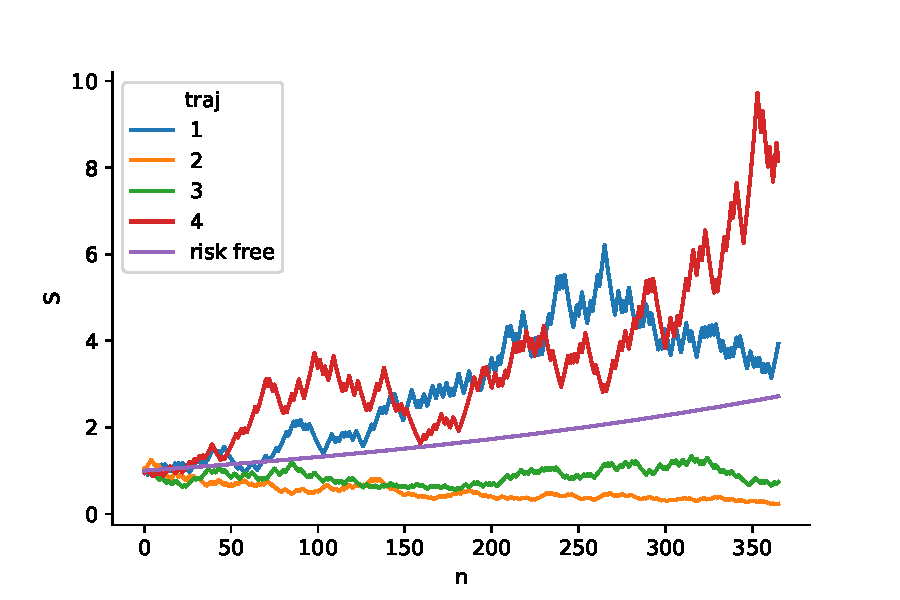
\includegraphics[width = \textwidth]{../Figures/traj_CRR.pdf}
\caption{Trajectoires du processus $S$ et de l'actif sans risque}
\label{fig:traj_CRR}
\end{figure}

Par analogie avec le modèle binomial, sous la probabilité risque neutre $\Q$, le processus $\tilde{S}_n = S_n/R_N^n,\text{ }n\geq0$ doit être une martingale pour la filtration $\mathcal{F}_n = \sigma_N(\xi_i, i\leq n)$. Le processus $\tilde S$ est une martingale sous $\Q$ si
$$
\E_\Q(\tilde{S}_{n+1}|\F_{n}) =  \tilde S_{n}.
$$
On observe que 
\begin{eqnarray*}
\E_\Q(\tilde{S}_{n+1}|\F_{n})& =& \E_\Q\left[\frac{S_{n}}{R_N^{n+1}}\e^{\mu_N + \xi_{n+1}\sigma_N}\Big|\F_{n}\right]\\
& =& \frac{S_{n}}{R_N^{n+1}}\e^{\mu_N}\E_\Q\left[\e^{\xi_{n+1}\sigma_N}|\F_{n}\right]\\
& =& \tilde S_{n}\frac{\e^{\mu_N}}{R_N}\E_\Q\left[\e^{\xi_{n+1}\sigma_N}\right]\\
& =& \tilde S_{n}\frac{q\e^{\mu_N+\sigma_N}+ (1-q)\e^{\mu_N-\sigma_N} }{R_N}\\
\end{eqnarray*}
Pour que $S$ soit une martingale, il faut que 
$$
q\e^{\mu_N+\sigma_N}+ (1-q)\e^{\mu_N-\sigma_N} = R_N \Leftrightarrow q = \frac{R_N-\e^{\mu_N-\sigma_N}}{\e^{\mu_N+\sigma_N}-\e^{\mu_N-\sigma_N}}.
$$
On a bien identifié la probabilité risque neutre $\Q$ telle que 
$$
\Q(\xi = 1) = \frac{R_N-e^{\mu_N-\sigma_N}}{\e^{\mu_N+\sigma_N}-\e^{\mu_N-\sigma_N}}=\frac{R_N-d}{u-d}=q
$$
de manière analogue au modèle binomial. La valorisation d'un produit dérivé de \textit{pay-off} $g(S_N)$ se fait sous la probabilité risque neutre avec 
$$
\pi = R_N^{-N}\mathbb{E}_\Q[g(S_N)].
$$ 
Cette espérance se calcule bien en remarquant que 
$$
\Q\left(S_N = S_0u^kd^{N-k}\right) = \binom{N}{k}q^k(1-q)^{N-k},\text{ pour }k = 0,\ldots, N.
$$
Prenons l'exemple du call européen avec $g(s) = (s-K)_+$. Soit 
\begin{equation}\label{eq:eta}
\eta_N =\inf\{k = 0,\ldots, N\text{ ; }S_0u^kd^{N-k}>K\},
\end{equation}
et $\bar{F}(n,p,k) = \Prob[\BinomialDist(n,p)> k]
$. On a 
\begin{equation}\label{eq:price_call_Binomial}
\pi = R_N^{-N}\mathbb{E}_\Q[(S_N-K)_+] = S_0\bar{F}\left(N,\frac{qu}{R_N},\eta_N\right)- R_N^{-N}K \bar{F}\left(N,q,\eta_N\right).
\end{equation}

\section{Annexes: Approximation normal dans le modèle de Cox-Rubinstein-Ross}
Le modèle de Cox-Ross-Rubinstein est une approximation d'un modèle en temps continu obtenu en laissant $N$ tendre vers l'infini. On note que sous la probabilité historique $\Prob$ et avec $p=1/2$, il vient
$$
\log\left(\frac{S_N}{S_0}\right) = N\mu_N+Z_N\sigma_N = \mu T + \frac{Z_N}{\sqrt{N}}\sigma\sqrt{T}\overset{\text{TCL}}{\sim}\NormalDist(\mu T, \sigma^2T)
$$
Les log rendements gaussien sont une caractéristique du modèle de Black-Scholes qu'on étudiera par la suite. Faire tendre $N$ vers l'infini permet également d'approcher le prix du call $\eqref{eq:price_call_Binomial}$. On a besoin du résultat suivant. 

\begin{lemma}
Soit $(X_n)_{n\geq0}$ une suite de \va indépendantes tel que $X_k\sim\BinomialDist(k, p_k)$ pour $k\geq1$ t alors 
$$
\frac{X_n-np_n}{\sqrt{np_n(1-p_n)}}\overset{\mathcal{D}}{\rightarrow}\NormalDist(0,1), \text{ lorsque }n\rightarrow\infty
$$
\end{lemma}
\begin{proof}
On montre que 
$$
\underset{n\rightarrow \infty}{\lim} \E(e^{tX_n})= \e^{t^2/2}.
$$
\end{proof}
D'après la définition de $\eta_N$, voir \eqref{eq:eta}, on a l'encadrement
$$
S_0u^{\eta_n-1}d^{N-\eta_n+1}\leq K\leq S_0u^{\eta_n}d^{N-\eta_n}.
$$
On en déduit en passant au log que  
$$
\eta_N\sigma\frac{\sqrt{T}}{\sqrt{N}} + N\left(\mu\frac{T}{N} - \sigma\frac{\sqrt{T}}{\sqrt{N}}\right) =\ln(K/S_0)+o(\sqrt{N})
$$
puis
$$
\eta_N = \frac{N}{2}+\frac{\sqrt{N}}{2\sigma\sqrt{T}}\left[\log(K/S_0)-\mu T\right]+ o(\sqrt{N})\text{, lorsque }N\rightarrow\infty.
$$
On a également
$$
q_{N} = \frac{e^{r\frac TN}-e^{\mu\frac TN-\sigma\sqrt{\frac{T}{N}}}}{e^{\mu\frac TN+\sigma\sqrt{\frac TN}} - e^{\mu\frac TN-\sigma\sqrt{\frac{T}{N}}}}
$$
Un développement limité à l'ordre 1 permet de conclure que $q_N\rightarrow 1/2$ pour $N\rightarrow +\infty$. Un développement limité à l'ordre 2 permet d'observer que 
$$
Nq_N = \frac{N}{2}+\frac{(r-\mu-\sigma^2/2)T}{2\sigma\sqrt{T}}\sqrt{N} + o(\sqrt{N})
$$
et de conclure que 
$$
\frac{\eta_N - Nq_N}{\sqrt{Nq_N(1-q_N)}} \rightarrow \frac{1}{\sigma\sqrt{T}}\left[\log(\widetilde{K}/S_0) + \sigma^2/2\right]= d^+,
$$
où $\widetilde{K} = Ke^{-rT}$. On a également 
$$
\frac{q_Nu_N}{R} = \frac{e^{r\frac TN}-e^{\mu\frac TN-\sigma\sqrt{\frac{T}{N}}}}{e^{\mu\frac TN+\sigma\sqrt{\frac TN}} - e^{\mu\frac TN-\sigma\sqrt{\frac{T}{N}}}}
\cdot 
\frac{e^{\mu\frac TN+\sigma\sqrt{\frac{T}{N}}}}{e^{r\frac TN}} = 
\frac{e^{(r+\mu)\frac TN+\sigma\sqrt{\frac TN}}-e^{2\mu\frac TN}}{e^{(r+\mu)\frac TN+\sigma\sqrt{\frac TN}} - e^{(r+\mu)\frac TN-\sigma\sqrt{\frac{T}{N}}}}
$$
Ce qui permet d'affirmer que 
$$\frac{q_Nu_N}{R}\rightarrow 1/2\text{, et }
N\frac{q_Nu_N}{R} = \frac{N}{2}+\frac{(r-\mu+\sigma^2/2)T}{2\sigma\sqrt{T}}\sqrt{N} + o(\sqrt{N})\text{ lorsque } N\rightarrow +\infty.
$$
Il vient alors 
$$
\frac{\eta_N - Nq_Nu_N/R}{\sqrt{Nq_Nu_N/R(1-q_Nu_N/R)}} \rightarrow \frac{1}{\sigma\sqrt{T}}\left[\log(\widetilde{K}/S_0) - \sigma^2/2\right] = d^-. 
$$
On conclut que 
$$
\pi_N\approx S_0[1-\phi(d^-)]- \widetilde{K} [1-\phi(d^+)].
$$
où $\phi(\cdot)$ est la fonction de répartition de la loi normal centrée réduite. On vérifie avec Python!

\section{Annexes: Blockchain, cryptomonnaie et double dépense}\label{app:application_blockchain}

Une blockchain est une base de données constituée de blocs successifs maintenue par un réseau pair-à-pair, comme sur la \cref{fig:blockchain_network}. 
\begin{figure}[ht!]
\begin{center}
\begin{tikzpicture}[-, >=, auto, semithick, node distance=01cm]
\tikzstyle{every edge}=[segment length=1mm,segment angle=10, draw]

\tikzstyle{full node}=[circle, fill=blue,draw=blue,thick,text=black,scale=0.8]
\tikzstyle{light node}=[circle, fill=white,draw=blue,thick,text=black,scale=0.8]
\node[full node]    (1)                     {};
\node[full node]    (2)[above right of=1]         {};
\node[full node]    (3)[above left of=1]         {};
\node[full node]    (4)[below of=1]         {};
\node[full node]    (5)[right of=4]         {};
\node[full node]    (6)[below of=4]         {};
\node[light node]    (7)[left of=1]         {};
\node[light node]    (8)[right of=2]         {};
\node[light node]    (9)[left of=4]         {};
\node[light node]    (10)[above right of=5]         {};
\node[light node]    (11)[ right of=5]         {};
\node[light node]    (12)[ below right of=5]         {};
% \node[light node]    (4)[above of=2]         {};
\path

(1) edge node{} (2)
    edge node{} (3)
    edge node{} (7)
    ;
\path
(5) edge node{} (10)
    edge node{} (11)
    edge node{} (12)
    ;
    \path
(4) edge node{} (5)
    edge node{} (1)
    edge node{} (9)
    edge node{} (6)
    ;
    \path
(2) edge node{} (8)   
    ;
\end{tikzpicture}
\end{center}
\caption{Un réseau fait de noeuds lourds (bleu) et de noeuds légers (blanc)}
\label{fig:blockchain_network}
\end{figure}
Les noeuds légers se contentent d'émettre des informations (appelées transactions). Les noeuds lourds doivent vérifier la cohérence des transactions et s'accorder sur les informations à inscrire dans la blockchain. Les noeuds lourds appliquent un protocole de consensus pour se mettre d'accord. La preuve de travail ou \textit{Proof-of-Work} est le protocole utilisé dans le cadre de la blockchain des bitcoins, voir le whitepaper de \citet{Nakamoto2008}. Un bloc doit être ajouté toutes les dix minutes environ, les noeuds sont en compétition pour résoudre un problème cryptographique brutalement via une méthode essai-erreur (\textit{trial and error}). Le premier qui parvient à résoudre le problème ajoute le bloc et récupère une récompense d'un montant de BTC$6.25$ à l'heure de l'écriture.\footnote{\url{https://bitcoinblockhalf.com/}}. \\

Dans la blockchain des bitcoins, les informations enregistrées sont des échanges de bitcoin entre les participants. Un noeud peut facilement émettre deux transactions conflictuelles, c'est à dire qui transfèrent les mêmes unités à deux entités différentes. Il s'agit d'une attaque par double dépense. Le scénario standard est le suivant:
\begin{enumerate}
    \item Marie transfère à John BTC$10$
    \item La transaction de Marie à John est enregistrée dans la blockchain
    \item John doit atendre $\alpha\in\N$ confirmations, c'est à dire que $\alpha$ blocs soient ajoutés après celui dans lequel la transaction de Marie à John est inscrite
    \item Une fois que $\alpha$ confirmations ont été envoyées, John envoie le bien à Marie
    \item Pendant ce temps, Marie travaille sur sa propre version de la blockchain (dite privée) dans laquelle la transaction de Marie à John est remplacée par une transaction de Marie à elle même
    \item Au moment de la livraison du bien la blockchain dite principale est en avance de $z$ blocs 
    \item L'objectif de Marie est générer une chaine concurrente plus longue que la chaine principale. Si elle y parvient, elle la communiquera à l'ensemble du réseau pour créer une fourche (\textit{fork}). Le réseau optera alors pour la branche la plus longue.
    La branche de Marie va alors remplacer la branche principale permettant à Marie de récupérer ses unités qu'elle peut dépenser à nouveau. 
\end{enumerate}
Cette course entre les deux branches est résumée sur la \cref{fig:dp_illustration}.
\begin{figure}[ht!]
\begin{center}
\begin{tikzpicture}[-, >=stealth', auto, semithick, node distance=1cm]
% \tikzstyle{block} = [rectangle, draw, fill=blue!20,
%     text width=5em, text centered, rounded corners]
\tikzstyle{block}=[rectangle, fill=black,draw=black,thick,text=black,scale=1.5]
\tikzstyle{block}=[rectangle, fill=white,draw=black,thick,text=black,scale=1.5]
\tikzstyle{confirmed block}=[rectangle, fill=white,draw=blue,thick,text=black,scale=1.5]
\tikzstyle{bad block}=[rectangle, fill=white,draw=red,thick,text=black,scale=1.5]
\node[block]    (1)                     {\tiny $\text{M}\rightarrow \text{J}$};
\node[block]    (2)[right of=1]                     {};
\node[block]    (3)[right of=2]                     {};
\node[block]    (4)[right of=3]                     {};
\node[confirmed block]    (5)[right of=4]                     {};

\node[bad block]    (6)[below of=1]         {\tiny $\text{M}\rightarrow \text{M}$};
\node[block]    (7)[right of=6]         {};
\node[block]    (8)[right of=7]         {};
\path
(1) edge[ left]     node{}     (2)
(2) edge[ left]     node{}     (3)
(3) edge[ left]     node{}     (4)
(4) edge[ left]     node{}     (5)
(6) edge[ left]     node{}     (7)
(7) edge[ left]     node{}     (8);

\end{tikzpicture}
\end{center}
\caption{La course à la double dépense illustrée, ici nous avons $\alpha = 4$ et $z = 2$}
\label{fig:dp_illustration}
\end{figure}
Notre objectif est de calculer la probabilité que la branche de Marie devienne majoritaire. Soit $(Z_n)_{n\in\mathbb{N}}$ la différence de longueur entre la branche de Marie et la branche principale de la blockchain. On a $Z_0 = z\geq 0$ et la double dépense se produit à l'instant aléatoire
\begin{equation}\label{eq:dp_time}
\tau_0 = \inf\{n\geq0\text{ ; }Z_n = 0\}.
\end{equation}
Nous souhaitons étudié la distribution de $\tau_0$ et en particulier calculer la probabilité de double dépense définie par 
\begin{equation}\label{eq:dp_prob}
\phi(z) = \Prob(\tau_0 <\infty|Z_0 = z) := \Prob_z(\tau_0 <\infty)
\end{equation}
A chaque instant $k\in\N$ un bloc est ajouté, il appartient 
\begin{itemize}
    \item A la branche principale avec probabilité $p\in(0,1)$
    \item à la branche de Marie avec probabilité $1-p$
\end{itemize}
Soit $(\Omega,\F, \Prob)$ un espace probabilisé. On définit une suite $(\xi_n)_{n\geq0}$ \iid de variables aléatoires (\va) de loi 
$$
\mathbb{P}(\xi = 1) = p\text{, et }\mathbb{P}(\xi = -1) = 1-p.
$$
On en déduit que 
$$
Z_n = z +\sum_{k=1}^n\xi_k.
$$
Le processus $Z_n$ est un processus à temps discret et à valeur dans $\Z$. Une visualisation du problème de premier passage est donné sur la \cref{fig:double_spending_time}.
\begin{figure}[ht!]
\begin{center}
\begin{tikzpicture}
  %Origin and axis
  \coordinate (O) at (0,0);
  \draw[->] (-1,0) -- (9,0) coordinate[label = {below:$n$}] (xmax);
  \draw[->] (0,-0.5) -- (0,3) coordinate[label = {left:$Z_n$}] (ymax);
  %Lower linear boundary

 
  %Stochastic process trajectory
  
  \draw (0,0) node[blue,left] {} node{};
  \draw[very thick,blue,-] (0,1) -- (1,1) node[pos=0.5, above] {} ;
  \draw[very thick,dashed,blue] (1,1) -- (1,1.5) node[pos=0.5, right] {};
  \draw[very thick,blue,-] (1,1.5) -- (2,1.5) node[pos=0.5, above] {};
  \draw[very thick,dashed,blue] (2,1.5) -- (2,2) node[pos=0.5, right] {};
  \draw[very thick,blue,-] (2,2) -- (3,2) node[pos=0.5, above] {};
  \draw[very thick,dashed,blue] (3,2) -- (3,1.5) node[pos=0.5, right] {};
  \draw[very thick,blue,-] (3,1.5) -- (4,1.5)node[pos=0.5, above] {};
  \draw[very thick,dashed,blue] (4,1.5) -- (4,1) node[pos=0.5, right] {};  
  \draw[very thick,blue,-] (4,1) -- (5,1) node[pos=0.5, above] {};
  \draw[very thick,dashed,blue] (5,1) -- (5,0.5) node[pos=0.5, right] {};  
  \draw[very thick,blue,-] (5,0.5) -- (6,0.5) node[pos=0.5, above] {};
  \draw[very thick,dashed,blue,-] (6,0.5) -- (6,1) node[pos=0.5, above] {};
   \draw[very thick,blue,-] (6,1) -- (7,1) node[pos=0.5, above] {};
    \draw[very thick,dashed,blue,-] (7,1) -- (7,0.5) node[pos=0.5, above] {};
     \draw[very thick,blue,-] (7,0.5) -- (8,0.5) node[pos=0.5, above] {};
     \draw[very thick,dashed,blue,-] (8,0.5) -- (8,0) node[pos=0.5, above] {};
  %Jump Times
  \draw (1,0) node[black,below] {$1$} node{ \color{black}$\bullet$};
  \draw (2,0) node[black,below] {$2$} node{ \color{black}$\bullet$};
  \draw (3,0) node[black,below] {$3$} node{ \color{black}$\bullet$};
  \draw (4,0) node[black,below] {$4$} node{ \color{black}$\bullet$};
  \draw (5,0) node[black,below] {$5$} node{ \color{black}$\bullet$};
  \draw (6,0) node[black,below] {$6$} node{ \color{black}$\bullet$};
  \draw (7,0) node[black,below] {$7$} node{ \color{black}$\bullet$};
  \draw (8,0) node[black,below] {$8$} node{ \color{black}$\bullet$};
  %Level of the counting process
   \draw (0,0) node[black,below left] {$0$} node{ \color{black}$\bullet$};
   \draw (0,0.5) node[black,left] {$1$} node{ \color{black}$\bullet$};
   \draw (0,1) node[black,left] {$z=2$} node{ \color{black}$\bullet$};
   \draw (0,1.5) node[black,left] {$3$} node{ \color{black}$\bullet$};
   \draw (0,2) node[black,left] {$4$} node{ \color{black}$\bullet$};
   \draw (0,2.5) node[black,left] {$5$} node{ \color{black}$\bullet$};

  % %Aggregated Capital gains
%  \draw (0,1.5) node[blue,below right] {$\mu_1$} node{ \color{blue}$-$};
%  \draw (0,2.25) node[blue,left] {$\mu_2$} node{ \color{blue}$-$};
%  \draw (0,3.75) node[blue,left] {$\mu_3$} node{ \color{blue}$-$};
  %Ruin time = First-crossing time time
%  \draw (5,0) node[black,above right] {${\tau_0}_u$} node{ \color{black}$\times$};
%  \draw[dotted,black] (0,3.28) -- (5,3.28);
%  \draw[dotted,black] (5,0) -- (5,3.28);
\end{tikzpicture}
\end{center}
\caption{Illustration du problème de premier passage sous-jacent à la double dépense.}
\label{fig:double_spending_time}
\end{figure}
L'application du \cref{theo_ruin_proba} avec $a\rightarrow \infty$ permet de résoudre le problème avec 
$$
\phi(z) = \left(\frac qp\right)^z.
$$

% \section{Annexes: Récurrence de la marche aléatoire sur $\mathbb{Z}$}\label{app:recurrence}

\section{Annexes: Convergence des Martingales}\label{app:convergence_martingale}
Cette section présente des résultats sur l'existence d'une loi limite pour les processus martingales. Soit $X=(X_n)_{n\geq 0}$ un processus défini sur un espace $(\Omega, \mathcal{F},\mathbb{P})$ adapté à la filtration $\mathcal{F}_n$ tel que $X_n$ est intégrable pour tout $n\geq 0$.
\begin{theo}\label{theo:convergence_ps_martingale}[De convergence des martingales]
Si $(X_n)_{n\geq0}$ est une S-martingale bornée dans $L^1$, c'est à dire telle que 
$$
\underset{n\in\mathbb{N}}{\sup}\E[(X_n)_+]<\infty,
$$ 
alors $X_n$ converge presque sûrement et dans $L^1$ vers une \va intégrable $X_\infty$.

\end{theo}
\begin{proof}
La démonstration du résultat nécessite de montrer un lemme pour lequel nous avons besoin d'introduire les objets suivants. Soit $a<b$ deux réels, on note 
\begin{itemize}
    \item $S_0 = T_0 = 0$,
    \item $S_1 = \inf\{n\geq 0\text{ : }X_n\leq a\}$ et $T_1 = \inf\{n> S_1\text{ : }X_n\geq b\}$,
    \item $S_{m+1} = \inf\{n> T_m\text{ : }X_n\leq a\}$ et $T_{m+1} = \inf\{n> S_m\text{ : }X_n\geq b\}$,
\end{itemize}
Pour tout $N\in \mathbb{N}$, on pose $M  = \sup\{m\geq 0, T_m \geq N\}$, noté $M_{N}(a,b)$ qui correspond au nombre de traversées montantes de l'intervalle $(a,b)$ par le processus $X$ jusqu'au temps $N$, en effet, on a 
$$
X_{S_{1}}\leq a,\,X_{T_{1}}\geq b,\ldots, X_{S_{M}}\leq a,  X_{T_{M}}\geq b.
$$

\begin{lemma}
Si $X$ est une sur-martingale alors 
$$
(b-a)\E\left[M_N(a,b)\right]\leq \E[(X_N-a)_
{-}],
$$
où $(x)_{-} = -\min(0,x)$ est la partie négative de $x$.

\end{lemma}
\begin{proof}
TODO
\end{proof}
Montrons le théorème dans le cas d'une sur-martingale . Le cas d'une sous-martingale s'en déduit car si $X$ est unue sous-martingale, bornée dans $L^1$ alors $Y  = -X$ est une sur-martingale bornée dans $L^1$ et le résultat s'applique. Pour une trajectoire $n\mapsto X_n(\omega)$ jusqu'au temps, le nombre de traversées montante $M_N(a,b)$ est une suite croissante en $N$, on note 
$$
M(a,b) = \underset{N\geq 0}{\sup} M_N(a,b).
$$ 
On remarque que 
$$
(b-a)\E[M_N(a,b)]\leq \E[(X_n-a)_{-}]\leq\E(|X_N|) + |a|\leq  \underset{N\geq 0}{\sup}\E(|X_N|) + |a|<\infty
$$
Cela implique qie $M(a,b)$ est fini presque surement. Si $X$ ne converge pas dans $\overline{\mathbb{R}} = \mathbb{R}\cup \{-\infty, +\infty\}$ lorsque $n\rightarrow\infty$ pour une trajectoire $\omega$, alors on a 
$$
\underset{n\rightarrow \infty}{\liminf}\, X_n(\omega) < \underset{n\rightarrow \infty}{\limsup}\, X_n(\omega). 
$$
Il existe alors deux rationnels $a<b$ tels que 
$$
\underset{n\rightarrow \infty}{\liminf}\, X_n(\omega) < a < b \underset{n\rightarrow \infty}{\limsup}\, X_n(\omega). 
$$
Dans ce cas $M(a,b) = \infty$, cela signifie que $\omega$ appartient à un ensemble de probabilité nulle. Par contraposée, le processus $X$ converge sauf sur des ensemble de mesure nulle et donc presque surement. De plus, on a 
$$
\E(|X_\infty|) = \E(\underset{n\rightarrow\infty}{\lim} |X_n|) = \E(\underset{n\rightarrow\infty}{\liminf} \,|X_n|)\underset{\text{Lemme de Fatou}}{\leq} \underset{n\rightarrow\infty}{\liminf}\,\E( |X_n|)\leq \underset{n\geq 0}{\sup}\,\E(|X_n|)< \infty.
$$

\end{proof}
On déduit du théorème précédent le corollaire suivant:
\begin{coro}
Soit $X$ une sur-martingale positive alors 
$$
X_\infty := \underset{n\rightarrow\infty}{\lim} X_n\text{ existe presque surement,}
$$
et vérifie $X_n \geq  \E(X_\infty|\F_n)$.
\end{coro}
\begin{proof}
Une sur-martingale positive est bornée dans $L^1$ donc le \cref{theo:convergence_ps_martingale} s'applique.
\end{proof}
Dans la suite nous avons besoin de la notion d'uniforme intégrabilité (UI). 
\begin{definition}
Le processus $X$ est uniformément intégrable (UI) si 
$$
\underset{M\rightarrow\infty}{\lim}\,\underset{n\geq 0}{\sup}\,\E(|X_n|\mathbb{I}_{|X_n|>M}) = 0
$$
Cela équivaut à 
$$
\forall \epsilon >0, \exists M >0,\forall n\geq 0,  \E(|X_n|\mathbb{I}_{|X_n|>M}) <\epsilon
$$
\end{definition}
\begin{ex}
Un processus $X$ dominé par une \va intégrable $Y$ est UI. En effet, pour tout $n\geq 0$
$$
\E(|X_n|\mathbb{I}_{[|X_n|>M})\leq \E(|Y|\mathbb{I}_{[|X_n|>M})\leq \E(|Y|\mathbb{I}_{[|Y|>M})
$$
On note que $\E(|Y|) = \E(|Y|\mathbb{I}_{|Y|\leq M} + \mathbb{I}_{|Y|>M})$ et $\underset{M\rightarrow \infty}{\lim}\, \E(|Y|\mathbb{I}_{[|Y|\leq M}) = \E(|Y|)$ cela implique que  
$$
 \underset{M\rightarrow \infty}{\lim}\E(|Y|\mathbb{I}_{[|Y|>M}) = 0.
$$
En particulier, le processus 
$$
X_n = \E(Y|\mathcal{F}_n),\text{ }n\geq 0,
$$
est une martingale UI.
\end{ex}
Une notion proche de l'uniforme intégrabilité est l'équi-intégrabilité
\begin{definition}
Le processus $X$ est equi-intégrable (EI) si 
$$
\forall \epsilon >0, \exists \eta >0, \forall A\in\mathcal{F}, \forall n\geq 0,\Prob(A)<\eta\Rightarrow \E(|X|\mathbb{I}_A) <\epsilon
$$
\end{definition}
La convergence des martingales est liée au fait que le processus soit bornée dans $L^1$, le résultat fait le lien entre uniforme intégrabilité et le fait que $X$ soit borné dans $L^1$. 
\begin{prop}
Soit $X$ un processus intégrable, les assertions suivantes sont intégrables 
\begin{itemize}
    \item[(i)] $X$ est UI
    \item[(ii)] $X$ est borné dans $L^1$ et $X$ est EI.
\end{itemize}
\end{prop}
\begin{proof}
TODO
\end{proof}
La notion d'uniforme intégrabilité permet de faire le pont entre convergence dans $L^1$ et convergence en probabilité. 
\begin{theo}
Soit $X$ un processus et $X_\infty$ une \va intégrable, les assertions suivantes sont équivalentes
\begin{itemize}
    \item[(i)] $X$ est UI et $X_n\overset{\Prob}{\rightarrow} X_{\infty}$. 
    \item[(ii)] $X$ est intégrable et $X_n\overset{L^1}{\rightarrow} X_{\infty}$. 
\end{itemize}
\end{theo}
\begin{proof}
TODO
\end{proof}
Avant de poursuivre, on introduit la notion de S-martingale fermée.
\begin{definition}
Une S-martingale $X$ est fermée à droite par une \va intégrable $Z$ si 
$$
\E(Z|\F_n)= X_n (\text{resp }\geq X_n\text{ ou }\leq X_n) 
$$
dans le cas d'une martingale (resp. d'une sous ou sur - martingale)
\end{definition}
On peut connecter la notion de martingale fermée et UI via le résultat suivant 
\begin{prop}
Soit $Z$ une \va intégrable alors la martingale définie par 
$$
X_n  = \E(Z|\F_n)
$$
est UI. 
\end{prop}
\begin{proof}
On a $X_n \leq Z_n  = \E(Z|\F_n)$, on a pour tout $n\geq 0$, 
$$
\E(X_n\mathbb{I}_{|X_n|>M})\leq \E(Z_n\mathbb{I}_{|Z_n|>M}) = \E(|Y|\mathbb{I}_{|Z_n|>M})
$$
Il faut démontrer que 
$$
\underset{M\rightarrow \infty}{\lim}\underset{n\geq 0}{\sup}\,\E(|Y|\mathbb{I}_{|Z_n|<M}).
$$
On a, pour $N, M>0$ 
\begin{eqnarray*}
\E(|Y|\mathbb{I}_{|Z_n|>M})&=& \E(|Y|\mathbb{I}_{|Z_n|>M, |Y|\leq N}) + \E(|Y|\mathbb{I}_{|Z_n|>M, |Y|> N})\\
&\leq& N \Prob(|Z_n|>M) + \E(|Y|\mathbb{I}_{|Y|> N})\\
&\underset{\text{Markov}}{\leq}& N\frac{\E(|Z_n|)}{M} + \E(|Y|\mathbb{I}_{|Y|> N})\\
&\underset{\text{Jensen}}{\leq}& N\frac{\E(|Y|)}{M} + \E(|Y|\mathbb{I}_{|Y|> N})\\
\end{eqnarray*}
pour tout $\epsilon >0$, il existe $N$ tel que $\E(|Y|\mathbb{I}_{|Y|> N})<\epsilon / 2$ (comme $Y$ est intégrable, c'est possible). On choisit alors $M =\frac{\E(2|Y|)N}{\epsilon}$, il vient 
$$
\underset{n\geq 0}{\sup}\,\E(|Y|\mathbb{I}_{|Z_n|<M})\leq \epsilon.
$$
\end{proof}
On peut énoncer le théorème de convergence suivant 
\begin{theo}
Soit $X$ une S-martingalme alors 
$$
X_n\overset{ L^1}{\longrightarrow}X_\infty\Leftrightarrow
 X\text{ est UI}$$
 Dans ce cas, $X$ converge presque sûrement vers $X_\infty$ et est fermée à droite par $X_\infty$
\end{theo}
\begin{proof}
TODO
\end{proof}
\begin{coro}
Soit $X$ une martingale, Les assertions suivnates sont équivalentes
\begin{itemize}
    \item[(i)] $X$ est UI
    \item[(ii)] $X_n\overset{ L^1}{\longrightarrow}X_\infty$
    \item[(iii)] $X$ est fermée à droite : $\exists Z\in L^1, \forall n\geq 0, \E(Z|\F_n) = X_n$
\end{itemize}
\end{coro}
\begin{proof}
TODO
\end{proof}
On peut aussi énoncer uun théorème d'arrêt avec des temps d'arrêt quelconques (pas nécessairement bornés)
\begin{theo}
Supposons que $X$ est une S-martingale UI alors pour deux temps d'arrêt (quelconques) tels que $\sigma\leq \tau$, on a 
$$
\E(X_\tau|\F_\sigma)= X_\sigma (\text{resp }\geq X_\sigma\text{ ou }\leq X_\sigma) 
$$
dans le cas d'une martingale (resp. d'une sous ou sur - martingale). En zparticulier, on a 
$$
\E(X_\infty|\F_\sigma) = X_\sigma.
$$
\end{theo}
\begin{proof}
TODO
\end{proof}

% \bibliography{includes/calcul_sto_chap_I}
% \bibliographystyle{plainnat}
% \section{Annexes: Un problème de contrôle optimal}
% La richesse d'une entreprise est modélisée par la marche aléatoire suivante
% $$
% X_{n+1} = X_n +\xi_{n+1}, \text{ }n\geq 0
% $$
% avec $X_0 = x$ et $(\xi_{n})_{n\geq1}$ une suite de \va \iid. On va supposer que $c\in\mathbb{N}$ et que les $\xi_i$ sint de \va discrète à valeurs dans $\mathbb{Z}$ telles que 
% $$
% \Prob(\xi_1 = i) = p_i\text{, }i\in\mathbb{Z},
% $$
% de sorte que $X_n\in \mathbb{Z}$. C'est un modèle doublement discret (en temps et en espace). Une partie de la richesse de l'entreprise doit être reversé aux actionnaire à cahque pas de temps sous la forme de dividende vu comme une suite de \va notée $(D_n)_{n\geq 0}$. Cela modifie la richesse de l'enstreprise qui devient 
% \begin{equation}\label{eq:controlled_process}
% \tilde{X}_{n+1} = \tilde{X}_n - D_n +\xi_{n+1}, \text{ }n\geq 0.
% \end{equation}
% Le montant de dividende est à la discrétion des dirigeants de l'entreprise et se réduit à une fonction $w$ telle que 
% $$
% D_n = w(\tilde{X}_n)<\tilde{X}_n.
% $$
% Le processus $(\tilde{X}_n)_{n\geq0}$ est le processus de richesse dit contrôlé, où $D_n$ est le contrôle. Soit 
% $$
% \tau_0 = \inf\{n\geq 0\text{ ; }X_n =0\},
% $$
% le temps de ruine, premier instant pour lequel la richesse modifiée pass en dessous de $0$. Soit $\delta>0$ le facteur d'actualisation et 
% $$
% V(x,w) =\E\left(\sum_{n =0}^{\tau- 1 }\delta^n D_n\right),
% $$
% l'espérance du cumul du montant actualisé des dividendes jusqu'à la cessation d'activité (ici la banqueroute). L'objectif des dirigeants est de définir une stratégie $w$ qui maximise $V(x,w)$, c'eest à dire permettant d'atteindre la cible 
% $$
% V(x) = \underset{w}{\sup} V(x,w).
% $$
% \begin{definition}\label{def:undominated_strategy}
% Une stratégie $w^\ast$ domine une startégie $w$ si 
% \begin{enumerate}
%     \item $V(x,w^\ast)\geq V(x,w)$ pour tout $x\geq 0$
%     \item $V(x,w^\ast)> V(x,w)$ pour certain $x\geq 0$
% \end{enumerate}
% Une stratégie "dominante" n'est dominée par aucune autre stratégie. 
% \end{definition}

% \subsection{ Exemple de stratégie}
% Une stratégie classique est du type \textit{band}.
% \begin{definition}
% Une \textit{band strategy} est la donnée de $2k+1$ entiers $a_0 <b_1<a_2<\ldots <b_n< a_n$ de sorte que le montant de dividendes versé aux actionnaires est défini par 
% $$
% D_n = w(\tilde{X}_n) = \begin{cases}
% 0,&\text{ si }\tilde{X}_n \geq a_0\text{ et }b_l\leq \tilde{X}_n\leq a_l\text{ pour }l = 1,\ldots, k.\\
% \tilde{X}_n - a_{l-1},&\text{ si }a_{l-1}\leq \tilde{X}_{n}\leq b_l\text{ pour }l = 1,\ldots, k,\\
% \tilde{X}_n - a_{k}, &\text{ si }\tilde{X}_{n} > a_{k}.
% \end{cases}
% $$
% \end{definition}
% La \textit{band strategy} est illustrée sur le schéma \cref{fig:band_strategy} avecc une trajectoire de $(\tilde{X}_n)_{n\geq 0}$.
% \begin{figure}[!ht]
% \begin{center}
% \begin{tikzpicture}
%     \begin{axis}[
%         axis lines = left,
%         xlabel = Time,
%         ylabel = {Capital},
%         ymin=0, ymax=140,
%         xmin=0, xmax=10,
%         ytick={30,60,90,120},
%         yticklabels={$a_0$, $b_1$, $a_1$, $b_2$},
%         xtick={0,1,...,9},
%         clip=false,
%         ]

%         % Upper and lower band lines
%         \addplot[domain=0:10, color=red, dashed] {120};
%         \addplot[domain=0:10, color=blue, dashed] {90};
%         \addplot[domain=0:10, color=green, dashed] {60};
%         \addplot[domain=0:10, color=orange, dashed] {30};

%         % Capital over time as a random walk
%         \addplot[mark=*,mark options={fill=black}] coordinates {
%             (0,50) (0,30) (1,65) (2,80) (3,70) (4,100) (4,90) (5,75) (6,80) (7,50) (7,30) (8,130) (9,110) (9,90) (10,85)
%         };

%         % Dividend payout points
%         % \draw[dashed] (axis cs:7,85) -- (axis cs:7,60);
%         % \draw[dashed] (axis cs:8,90) -- (axis cs:8,60);

%         % \node at (axis cs:7,25) [anchor=north] {Dividend Payout};
%         % \node at (axis cs:8,25) [anchor=north] {Dividend Payout};
%     \end{axis}
% \end{tikzpicture}
% \end{center}
% \caption{Trajectoire du processsus contrôlé $(\tilde{X}_n)_{n\geq 0}$.}
% \label{fig:band_strategy}
% \end{figure}

% \noindent L'existence d'une \textit{band strategy} optimale dans le cadre de notre modèle a été prouvé par exemple dans \citet[Theorem 1]{Gerber1972}. Il n'est cependant pas évident de trouver les bornes définissant les bandes explicitement. C'est plus facile dans le cas où $k=0$ qui correspond à une stratégie dite barrière. Lorsque la richesse excède le seuil $a:=a_0$, le surplus est reversé aux actionnaires. L'existence d'une stratégie barrière a été démontré dans le travail de \citet{Miyasawa1961} lorsque 
% $$
% p_i = 0\text{ pour } i \leq -2.
% $$
% Dans \citet{Gerber1972}, il est démontré l'existence qu'une stratégie barrière de niveau $a$ est localement optimale c'est à dire optimale pour certain niveau de capital initial $x =0,\ldots, a$, lorsque 
% $$
% p_i = 0\text{ pour } i \geq 2.
% $$
% On va se contenter d'établir l'optimalité de la stratégie barrière dans le cas d'une marche aléatoire simple dans la section \cref{subsec:optimality_band_strategy}
% La détermination explicite du seuil de la barrière et du montant espéré des dividendes est effectuée dans la section \cref{subsec:dividen_RW}.
% \subsection{Optimalité de la stratégie barrière dans le cas de la marche aléatoire simple}\label{subsec:optimality_band_strategy}
% On suppose que 
% $$
% \Prob(\xi_1 = 1) = p,\text{ }\Prob(\xi_1 = 1) = q = 1-p.
% $$
% La stratégie dominante $w^{\ast}$ doit vérifier l'équation suivante 
% \begin{equation}\label{eq:bellman_equation}
% V(x,w^\ast) = \max\left[\delta (pV(x+1,w^\ast) + qV(x-1,w^\ast)), \underset{1\leq y\leq x}{\max} y + V(x-y,w^\ast)\right],
% \end{equation}
% qui indique que l'entreprise au vu de son niveau de surplus peut entrer dans le nouvelle exercice en ne versant pas de dividendes ou en versement directement un montant 
% $$
% w^{\ast}(x) = y.
% $$
% L'équation fonctionnelle \eqref{eq:bellman_equation} est l'équation vérifié par $V$ est appelée équation de Bellman. Il s'agit d'une application du principe de la programation dynamique qui exprime que la solution optimale est déterminer par une stratégie permettant de passer d'une période à une autre. Il est possible que les termes $\delta (pV(x+1,w^\ast) + qV(x-1,w^\ast))$ et  $\underset{1\leq y\leq x}{\max} y + V(x-y,w^\ast)$ soient égaux, nous adoptons la convention suivante 
% \begin{equation}\label{eq:strategie_speciale}
% w^\ast(x) = 0 \Leftrightarrow \delta (pV(x+1,w^\ast) + qV(x-1,w^\ast)) >  \underset{1\leq y\leq x}{\max} y + V(x-y,w^\ast)
% \end{equation}
% qui stipule qu'en cas d'égalité, on préfère payer des dividendes immédiatement. On peut ré-écrire \eqref{eq:bellman_equation} comme 
% \begin{equation}\label{eq:eq:bellman_equation2}
% V(x,w^\ast) =  \underset{0\leq y\leq x}{\max} y +  h(x-y, \omega^\ast), 
% \end{equation}
% où
% $$
% h(x, \omega^\ast) = \delta\left[ pV(x+1,w^\ast) + qV(x-1,w^\ast)\right].
% $$
% \begin{prop}\label{prop:properties_optimal_strategy}
% Soit $w^\ast$ une stratégie dominante.
% \begin{enumerate}
%     \item Il existe $x\in \mathbb{N}$ tel que $w^\ast(x) >0$
%     \item S'il existe $x,a$ et $b$ des entiers tels que $a<b$ et 
%     $$
%     w^\ast(x)=\begin{cases}
%     0,&\text{ pour }x \leq a, \\
%     >0,&\text{ pour }a<x <b,
%     \end{cases}
%     $$
%     alors 
%     $$
%     w^\ast(x)=\begin{cases}
%             0,&\text{ pour }x \leq a, \\
%             x-a,&\text{ pour }a<x\ <b,\\
%             \end{cases}
%             $$
% \end{enumerate}
% \end{prop}
% \begin{proof}
% \begin{enumerate}
%     \item Supposons que $w^\ast(x) = 0$ pour tout $x$ alors $V(x,w^\ast) = 0$. Or la stratégie $w'$ qui consiste à verser l'intégralité du capital restant en dividende est tel que 
%     $$
%     V(x,w') = x > V(x,w^\ast)\text{, pour }x\geq 1.
%     $$
%     ce qui contredit la domination bde $w^\ast$.
%     \item Par hypothèse $w^\ast(a) = 0$, on en déduit que 
% $$
% V(a,w^\ast) = \underset{y = 0,\ldots, a}{\max} y + h(a-y,w^\ast) = h(a,w^\ast).
% $$
% On considère 
% \begin{eqnarray*}
% V(a+1,w^\ast) &=& \underset{y = 0,\ldots, a+1}{\max} y + h(a+1-y,w^\ast))\\
% &=&\max(h(a+1,w^\ast), \underset{y = 1,\ldots, a+1}{\max} y + h(a+1-y,w^\ast))\\
% &=&\max(h(a+1,w^\ast), \underset{y = 0,\ldots, a}{\max} y +1 + h(a-y,w^\ast))\\
% &=&\max(h(a+1,w^\ast), 1+h(a,w^\ast))
% \end{eqnarray*}

% En itérant jusqu'à k tel que $a+k = b-1$ il vient 
% $$
% w^\ast(a+l) =l,\text{ pour }l = 1,\ldots, k.
% $$
% On a pour finir 

% \begin{eqnarray*}
% V(b,w^\ast) &=& \underset{y = 0,\ldots, a+1}{\max} y + h(b-y,w^\ast))\\
% &=&\max(h(b,w^\ast), \underset{y = 1,\ldots, a+1}{\max} y + h(a+1-y,w^\ast))\\
% &=&\max(h(a+1,w^\ast), \underset{y = 0,\ldots, a}{\max} y +1 + h(a-y,w^\ast))\\
% &=&\max(h(a+1,w^\ast), 1+h(a,w^\ast)).
% \end{eqnarray*}
% \end{enumerate}

% \end{proof}
%  La proposition indique l'existence d'un plus petit entier $a$ qui joue le rôle de barrière réfléchissante. La question est de savoir s'il existe $b >a$ tel que $w^\ast(b) = 0$ auquel cas on aurait aussi l'existence de $a_1>b$ tel que $w(a_1+1)>0$ par l'item $1$ et de plus $w(a_1+1) = 1$ par l'item $2$. On peut postuler une stratégie dominante telle que 
%  $$
% w^\ast(x)=\begin{cases}
%             0,&\text{ pour }x \leq a, \\
%             x-a,&\text{ pour }a<x\ <b,\\
%             0,& \text{ pour }b\leq x\leq a_1\\
%             1,\text{ pour }x = a_1+1
%             \end{cases}
%  $$
%  Il s'agit d'un embryon de stratégie de type bande. Pour que cette stratégie soit de type barrière il faut montrer que $b = \infty$. C'est l'objet du réusltat suivant. 
%  \begin{theo}
%  Dans le cas où la richesse est gouvernée par une marche aléatoire simple, on a $b = \infty$

%  \end{theo}
%  \begin{proof}
%  Supposons qu'il existe $b <\infty$ alors il existe également $a_1<\infty$ tel que $a_1>b$. On va montrer que l'on peut définir une stratégie $w'$ qu domine $w^\ast$. Notons $\tilde{X}^\ast_n$ et $\tilde{X}'_n$ les processus contrôlés en appliquant les stratégies $w^\ast$ et $w'$ respectivement. On note 
%  $$
%  \tau' = \inf\{n\geq 0\text{ ; }\tilde{X}'_n  = a_1\},
%  $$
%  et
% $$
%  \tau^\ast = \inf\{n\geq 0\text{ ; }\tilde{X}^\ast_n  = b\}.
%  $$

%  Soit 
%  $$
% w'(\tilde{X}'_n)=\begin{cases}
%             0,&\text{ pour }\tilde{X}'_n \leq a,\text{ ou }n = \tau' ,\\
%             \tilde{X}'_n-a,&\text{ pour }a<\tilde{X}'_n\ <b- 1,\text{  et } n <\tau', \\
%             \tilde{X}'_n-a,&\text{ pour }a\leq\tilde{X}'_n\leq b,\text{  et } n \geq \tau', \\
%             0,&\text{ pour }b-1<\tilde{X}'_n\ <a_1,\text{  et } n <\tau', \\
%             0,& \text{ pour }b\leq \tilde{X}'_n\leq a_1,\text{  et } n \geq \tau',\\
%             w^\ast (\tilde{X}'_n),&\text{ pour }\tilde{X}'_n = a_1+1.
%             \end{cases}
% $$

%  \end{proof}
%  Supposons que $X_0' = x$ et  $X_0^\ast = x+1$ avec $b\leq x <x+1\leq a_1$. On considère le scénario dans chacune des deux situations, c'est à dire des valeurs identiques pour les éléments de la suite $(\xi_n)_{n\geq 0}$. On étudie deux cas séparément. 

% \begin{enumerate}
%     \item Supposons que $X_n'$ atteigne $a_1$ (c'est l'instant $\tau'$) avant que $X_n^\ast$ n'atteigne le niveau $b-1$. On a $X{_\tau'}^\ast = X{_\tau'}^\ast$ et même $X_n' = X_n^\ast$ pour $n\geq \tau'$ puisque $w^\ast$ et $w'$ coincide. On observe que 
%     $$
%     V(x+1,w^\ast) - V(x,w') = \delta^{\tau'} \leq 1
%     $$
%     \item Supposons que $X_n'$ n'atteigne pas $a_1$ avant que $X_n^\ast$ n'atteigne le niveau $b-1$ (instant $\tau^\ast$). On a $X_{\tau^\ast} = X_{\tau^\ast}$ et même $X_n' = X_n^\ast$ pour $n\geq \tau^\ast$ puisque $w^\ast$ et $w'$ coincide. On observe que 
%     $$
%     V(x+1,w^\ast) - V(x,w') = \delta^{\tau^\ast} \leq 1
%     $$
% \end{enumerate}
% Dans les deux cas $w'$ domine $w^\ast$, en effet 
% $$
% V(x+1,w') - V(x,w') \geq 1
% $$
% et donc $V(x+1,w') \geq V(x+1,w^\ast)$. Cela contredit la domination de $w^\ast$. On a bien $b = \infty$.
% \begin{remark}
% La preuve est assez fastidieuse. Dans la pratique, une stratégie $w^\ast$ est optimale lorsque les deux condition suivantes sont vérifiées
% \begin{itemize}
%     \item[(i)] $V(x+1,w^\ast)\geq V(x,w^\ast) + 1$
%     \item[(ii)] $V(x,w^\ast)\geq h(x,w^\ast)$
% \end{itemize}
% Voir le raisonnement dans la preuve de 2. de \cref{prop:properties_optimal_strategy}. On peut alors déterminer la stratégie optimale en postulant cette stratégie puis en vérifiant que (i) et (ii) sont satisfaite. Il faut pour cela avoir une idée de la stratégie optimale, qui est souvent du type barrière ou bande pour les processus du type marche aléatoire ou processus de Lévy qui sont l'équivalent des marche aléatoire en temps continu (étudié dans le \cref{chap:processus_levy})
% \end{remark}
% \subsection{Détermination de la barrière optimale et du montant espéré de dividende pour la marche aléatoire sur $\mathbb{Z}$}\label{subsec:dividen_RW}
% Dans le cas de la marche aléatoire simple la stratégie optimale est une stratégie barrière de niveau $a$ pour laquel la fonction objectif vérifie
% $$
% V(x;a) = \delta\left[pV(x+1;a) + qpV(x-1;a)\right],\text{ pour }1\leq x\leq a.
% $$ 
% Il s'agit d'une équation récurrente linéaire d'ordre deux avec les conditions limites suivantes
% $$
% V(0;a) =0\text{ et }V(a+1; a) = 1 + V(a; a).
% $$
% Les solutions sont données par 
% $$
% V(x;a) = A_1 r_1^x + A_2 r_2^x,
% $$
% où $A_1$ et $A_2$ sont des constantes et $r_1$ et $r_2$ sont les racines du polynôme caractéristique
% $$
% \delta p r^2 - r + \delta q = 0.
% $$
% On en déduit que 
% $$
% r_1 = \frac{1 + \sqrt{\Delta}}{2\delta p }\text{, et }r_2 = \frac{1 - \sqrt{\Delta}}{2\delta p },
% $$
% avec $\Delta = 1 - 4 \delta^2p(1-p)$. Via les conditions limites, on obtient
% $$
% A_1 = -A_2\text{ et }A_1 = \frac{1}{(r_1^{a+1} -r_2^{a+1} ) - (r_1^{a} -r_2^{a} )}
% $$
% Il est intéressant d'observer que 
% $$
% V(x;a) = g(a)f(x),
% $$
% où
% $$
% g(a) = \frac{1}{(r_1^{a+1} -r_2^{a+1} ) - (r_1^{a} -r_2^{a} )}
% $$
% La valeur optimal du seuil coincide avec le maximum de la fonction $g$ et ne dépend pas de la réserve initiale $x$.
% \begin{remark}
% Une manière économique et probabiliste d'obtenir le résultat est de considérer la valeur actuelle probable d'un paiement de montant $1$ à l'instant 
% $$
% \tau_{a+1} = \inf\{n\geq 0\text{ }X_n = a\},
% $$
% sachant que $X_n = x\leq a$ et que la ruine ne s'est pas produite. On note
% $$
% C(x, a+1) = \E_x(\delta^{\tau_{a+1}}\mathbb{I}_{\tau_{a+1}<\tau_0}).
% $$
% La richesse de l'entreprise est une chaine de Markov homogène. de plus, comme $X_0 = 1$, $\tau_x < \tau_{a+1}$ pour $x\leq a+1$, alors on peut écrire
% \begin{eqnarray}\label{eq:factorization_formula}
% C(1, a+1) &=& \E_1(\delta^{\tau_{a+1}}\mathbb{I}_{\tau_{a+1}<\tau_0})\nonumber\\
% & = &\E_1\left[\E(\delta^{\tau_{a+1} - \tau_x + \tau_x}\mathbb{I}_{\tau_{a+1}<\tau_0}\mathbb{I}_{\tau_{x}<\tau_0}\rvert \mathcal{F}_{\tau_x})\right]\nonumber\\
% &=&\E_1\left[\delta^{\tau_x}\mathbb{I}_{\tau_{x}<\tau_0}\E(\delta^{\tau_{a+1} - \tau_x }\mathbb{I}_{\tau_{a+1}<\tau_0}\rvert \mathcal{F}_{\tau_x})\right]\nonumber\\
% &=&\E_1\left[\delta^{\tau_x}\mathbb{I}_{\tau_{x}<\tau_0}\right]\E_x[\delta^{\tau_{a+1}}\mathbb{I}_{\tau_{a+1}<\tau_0}]\nonumber\\
% &=&C(1, x)C(x, a+1).
% \end{eqnarray}
% On note 
% $$
% f(x) = \frac{1}{C(1,x)}\text{, } x\leq a,
% $$
% que l'on appelle la fonction d'échelle (en théorie de la fluctuation). Dans le cadre d'une stratégie barrière de niveau $a$ la fonction objectif vérifie
% $$
% V(x; a) = x-a+V(a+1; a)\text{, pour }x\geq a+1.
% $$
% Par un raisonnement similaire à \eqref{eq:factorization_formula}, il vient 
% $$
% V(x; a) = C(x, a+1)V(a+1;a) = \frac{C(1,a+1)}{C(1, x)}V(a+1;a) = f(x)g(a).
% $$
% Comme $V(a+1; a) - V(a; a) = 1$, on en déduit que 
% $$
% g(a) = \frac{1}{f(a+1) - f(a)}
% $$
% puis 
% $$
% V(x; a) = \frac{f(x)}{f(a+1) - f(a)}.
% $$




% \end{remark}

\bibliography{includes/calcul_sto_chap_I}
\bibliographystyle{plainnat}

% \begin{thebibliography}{6}
% \providecommand{\natexlab}[1]{#1}
% \providecommand{\url}[1]{\texttt{#1}}
% \expandafter\ifx\csname urlstyle\endcsname\relax
%   \providecommand{\doi}[1]{doi: #1}\else
%   \providecommand{\doi}{doi: \begingroup \urlstyle{rm}\Url}\fi

% \bibitem[Laleuf(2014)]{laleuf14}
% Jean-Claude Laleuf.
% \newblock \emph{Processus et intégrales stochastiques (Cours et exercices
%   corrigés)}.
% \newblock Paris, 2014.

% \bibitem[Le~Gall(2006)]{LeGall2006}
% Jean-Fran{\c{c}}ois Le~Gall.
% \newblock \emph{Int{\'e}gration, probabilit{\'e}s et processus al{\'e}atoires}.
% \newblock Ecole Normale Sup{\'e}rieure de Paris, 2006.

% \bibitem[Nakamoto(2008)]{Nakamoto2008}
% S.~Nakamoto.
% \newblock Bitcoin: A peer-to-peer electronic cash system.
% \newblock Available at
%   \href{https://bitcoin.org/bitcoin.pdf}{https://bitcoin.org/bitcoin.pdf},
%   2008.
% \newblock URL \url{https://bitcoin.org/bitcoin.pdf}.

% \bibitem[Tankov and Touzi(2010)]{Tankov2010}
% Peter Tankov and Nizar Touzi.
% \newblock Calcul stochastique en finance.
% \newblock \emph{Ecole Polytechnique Paris, D{\'e}partement de Math{\'e}matiques
%   Appliqu{\'e}es}, page 146, 2010.

% \bibitem[Truquet(2015)]{Truquet_stat_proc}
% Lionel Truquet.
% \newblock Statistiques des processus 3a.
% \newblock Lecture notes, 2015.
% \newblock
%   \url{https://ensai.fr/wp-content/uploads/2019/06/polystatdesprocessus2.pdf}.

% \bibitem[Williams(1991)]{Williams1991}
% David Williams.
% \newblock \emph{Probability with Martingales}.
% \newblock Cambridge University Press, feb 1991.
% \newblock \doi{10.1017/cbo9780511813658}.

% \end{thebibliography}

\newpage
% !TEX root = ../main_lecture_notes.tex
\chapter{Processus et martingale en temps continu}\label{chap:processus_levy}
On étend les notions de temps d'arrêt et de martingale aux processus à temps continu. Nous introduisons la notion de processus de Lévy qui sont l'équivalent de la marche aléatoire en temps continu. L'exemple fil rouge sera un modèle de gestion des risques des compagnies d'assurances basé sur le processus de Poisson composé. 
\section{Le modèle de ruine de Cramer-Lundberg}\label{sec:cramer-lundberg}
L'objectif est de proposer un modèle pour l'évolution de la richesse d'une compagnie d'assurance au cours du temps via un processus $X:=(X_t)_{t\geq0}$, avec $t\in\RL_+$. Une compagnie d'assurance détient un capital initial $x\geq0$, perçoit des primes de la part des assurés au taux $c>0$ et paie de temps à autre une indemnisation. Le nombre de sinistres jusqu'à l'instant $t$ est donnée par un processus de comptage $N:=(N_t)_{t\geq0}$. 
\begin{definition}\label{def:counting_process}
Un processus de comptage $(N_t)_{t\geq0}$ est un processus en temps continu qui compte le nombre d'occurence d'un évènement au cours du temps
\begin{equation*}
N_0=0\text{ et }N_t=\sum_{k=1}^{+\infty}\mathbb{I}_{T_k\leq t}.
\end{equation*}
où $T_1,T_2,T_3,\ldots$ désigne les temps d'arrivée des évènements, avec la convention $T_0=0$. Soit $\Delta^T_0,\Delta^T_1,\Delta^T_2,\ldots$ la suite des temps inter-arrivée définis par
$$
\Delta^T_k=T_{k+1}-T_{k}\text{, }k=0,1,2\ldots.
$$
\end{definition}
Un exemple de trajectoire d'un processus de comptage est donnée par la \cref{fig:trajectory_counting_process}
\begin{figure}[!h]
\begin{center}
\begin{tikzpicture}[scale=1]
  %Origin and axis
  \coordinate (O) at (0,0);
  \draw[->] (-1,0) -- (8,0) coordinate[label = {below:$t$}] (xmax);
  \draw[->] (0,-0.5) -- (0,5.5) coordinate[label = {left:$N_t$}] (ymax);
  %Lower linear boundary


  %Stochastic process trajectory

  \draw (0,0) node[blue,left] {} node{};
  \draw[very thick,blue,-] (0,0) -- (1,0) node[pos=0.5, above] {$\Delta^T_0$} ;
  \draw[very thick,dashed,blue] (1,0) -- (1,1) node[pos=0.5, right] {};
  \draw[very thick,blue,-] (1,1) -- (1.75,1) node[pos=0.5, above] {$\Delta^T_1$};
  \draw[very thick,dashed,blue] (1.75,1) -- (1.75,2) node[pos=0.5, right] {};
  \draw[very thick,blue,-] (1.75,2) -- (2.75,2) node[pos=0.5, above] {$\Delta^T_2$};
  \draw[very thick,dashed,blue] (2.75,2) -- (2.75,3) node[pos=0.5, right] {};
  \draw[very thick,blue,-] (2.75,3) -- (5,3)node[pos=0.5, above] {$\Delta^T_3$};
  \draw[very thick,dashed,blue] (5,3) -- (5,4) node[pos=0.5, right] {};
  \draw[very thick,blue,-] (5,4) -- (6,4) node[pos=0.5, above] {$\Delta^T_4$};
  \draw[very thick,dashed,blue] (6,4) -- (6,5) node[pos=0.5, right] {};
  \draw[very thick,blue,-] (6,5) -- (8,5) node[pos=0.5, above] {$\Delta^T_5$};
  %Jump Times
  \draw (1,0) node[blue,below] {$T_1$} node{ \color{blue}$\bullet$};
  \draw (1.75,0) node[blue,below] {$T_2$} node{ \color{blue}$\bullet$};
  \draw (2.75,0) node[blue,below] {$T_3$} node{ \color{blue}$\bullet$};
  \draw (5,0) node[blue,below] {$T_4$} node{ \color{blue}$\bullet$};
  \draw (6,0) node[blue,below] {$T_5$} node{ \color{blue}$\bullet$};
  %Level of the counting process
   \draw (0,0) node[black,left] {$0$} node{ \color{black}$\bullet$};
   \draw (0,1) node[black,left] {$1$} node{ \color{black}$\bullet$};
   \draw (0,2) node[black,left] {$2$} node{ \color{black}$\bullet$};
   \draw (0,3) node[black,left] {$3$} node{ \color{black}$\bullet$};
   \draw (0,4) node[black,left] {$4$} node{ \color{black}$\bullet$};
   \draw (0,5) node[black,left] {$5$} node{ \color{black}$\bullet$};
\end{tikzpicture}
\end{center}
\caption{Une trajectoire du processus de comptage $(N_t)_{t\geq0}$.}
\label{fig:trajectory_counting_process}
\end{figure}
\begin{definition}\label{def:exp_dist}
Une \va $X\sim\ExpDist(\lambda)$ est une \va continue de densité
$$
f_X(x) =\lambda\e^{-\lambda x}\ind_{(0,\infty)}.
$$
\end{definition}
\begin{definition}\label{def_poisson_process}
Un processus de Poisson $(N_t)_{t\geq0}$ d'intensité $\lambda$ est un processus de comptage dont les temps inter-arrivée \iid sont de loi exponentielle $\ExpDist(\lambda)$.
\end{definition}
\begin{remark}\label{def_renewal_process}
Le processus de Poisson appartient à la famille des processus de renouvellement qui sont des processus de comptage dont les temps inter-arrivée sont \iid.
\end{remark}
\begin{prop}
Soit $(N_t)_{t\geq 0}$ un processus de comptage, il y a équivalence entre les deux assertions suivantes:
\begin{itemize}
    \item[(i)] $(N_t)_{t\geq0}$ est un processus de Poisson d'intensité $\lambda$
    \item[(ii)] Les accroissements de $(N_t)_{t\geq 0}$ sont
    \begin{itemize}
        \item indépendants, c'est à dire $N_{t}-N_{s}$ et $N_s$ sont indépendants pour tous $s\leq t$,
        \item stationnaires c'est à dire que 
        $$
        N_t - N_s = N_{t-s}\sim\text{Pois}(\lambda\cdot(t-s)).
        $$
    \end{itemize}
\end{itemize}
On note que $N_t\sim\text{Pois}(\lambda t)$ et que $\lambda$ correspond au nombre moyen de sauts par unité de temps. 
\end{prop}
Dans le modèle considéré, l'arrivée des sinistres est modélisée par un processus de Poison $(N_t)_{t\geq0}$ d'intensité $\lambda>0$. Pour chaque sinistre une indemnisation est versée aux assurés. ces indemnisation forment une suite $(U_n)_{n\geq0}$ de \va \iid et positives. Finalement la richesse de la compagnie d'asssurance est donnée par 
\begin{equation}\label{eq:cramer_lundberg_modele}
X_t = x + ct - \sum_{k=1}^{N_t}U_k,\text{ }t\geq 0.
\end{equation}
Usuellement les primes sont reçues à la date d'anniversaire des contrats. Ici, on suppose que le portefeuille est suffisamment important pour pouvoir approcher l'encaissement des primes par une fonction linéaire de pente $c$. La gestion des risque repose souvent sur la définition d'une mesure de risque qui résume par un nombre le risque sous-jacent. En théorie du risque, on utilise la probablité de ruine à un horizon de temps $T\geq 0$ définie par 
$$
\psi(x,T) = \Prob\left(\tau_0^-\leq T\right),
$$
où $\tau_0^- = \inf\{t\geq 0\text{ ; }X_t\leq0\}$ est le premier instant pour lequel la richesse de l'assureur passe en dessous de $0$. L'objectif de l'actuaire est dès lors de déterminer un niveau de prime $c$ et une richesse initiale $x$ associé à un niveau de risque $\psi(x,T) = 1-\alpha$. La directive européenne Solvabilité II impose un niveau de risque $\alpha = 99.5\%$ à horizon de temps $T= 1 \text{an}$. Le niveau de prime compense le cout moyen des sinistre par unité de temps avec 
$$
c = (1+\eta)\frac{1}{t}\E\left(\sum_{k=1}^{N_t}U_k\right) = (1+\eta)\lambda\E(U),
$$
où $\eta>0$ est le chargement de sécurité (de combien la prime commercial ecxcède la prime pure). On définit également la probabilité de ruine ultime par 
$$
\psi(x) = \underset{T\rightarrow \infty}{\lim} \psi(x,T),
$$
nous verrons que si $\eta \leq 0$ alors $\psi(x) = 1$. Une fois le niveau de prime fixé, le seul paramètre à ajusté est le niveau de richesse initiale $x$ dont la détermination passe par l'évaluation numérique de la probabilité de ruine.
\section{Généralités sur les processus en temps continu}\label{sec:processus_continu}
\subsection{Définitions}\label{ssec:definitions}
Soit $(\Omega, \F, \Prob)$ un espace probabilisé. 
\begin{definition}\label{def:filtration}
Une filtration $(\F_t)_{t\geq0}$ est une suite croissante croissante pour l'inclusion avec
$$
\F_s\subset \F_t,\text{ pour }s\leq t,
$$
de sous-tribu de $\F$.
\end{definition}
Soit $(\F_t)_{t\geq0}$ une filtration de $(\Omega, \F, \Prob)$. $\F_t$ correspond à l'information disponible au temps $t$,
\begin{definition}\label{def:processus}
Une suite $(X_t)_{t\in \RL_+}$ de variable aléatoires (\va) sur $\Omega$ est un processus stochastique en temps continu. $X$ est $\F_t$-adapté si $X_t$ est mesurable par rapport à $\F_t$ pour tout $t\geq0$. 
\end{definition}
\begin{remark}
La filtration $\F_t$ associée à un processus $(X_t)_{t\geq 0}$ est l'information qu'il faut détenir pour pouvoir tracer la trajectoire du processus jusqu'à l'instant $t\geq 0$. Pour le processus de comptage, il s'agit des instants de saut 
$$
\F_t = \sigma[(\ind_{T_k \leq t})_{k\geq 0}].
$$
Pour le processus de richesse il faut ajouter la taille des sauts
$$
\F_t=\sigma[(U_k\ind_{T_k \leq t})_{k\geq 0}].
$$
\end{remark}
% \begin{definition}\label{def:processus_egaux}
% Deux processus $X$ et $Y$ sont égaux en loi, noté $X \overset{\mathcal{D}}{=} Y$, si 
% $$
% (X_{t_1}, \ldots, X_{t_n})\overset{\mathcal{D}}{=} (Y_{t_1}, \ldots, Y_{t_n}),\text{ pour tout } n\in \N\text{ et }(t_1,\ldots, t_n)\in \RL_+^n.
% $$
% \end{definition}
\subsection{Propriétés fonctionnelles}
Soit $\omega\in\Omega$,  est une trajectoire ou réalisation. Il s'agit d'une fonction du temps $t\mapsto X_t(\omega)$ dont on peut étudier les propriétés comme la monotonie, la continuité, et la dérivabilité 
\begin{itemize}
  \item Un processus $X$ est croissant la fonction $t\mapsto X_t$ est croissante presque surement (\ps).
  \item Un processus $X$ est continu à droite, continu, dérivable, de classe $\mathcal{C}^2$, $\ldots$ si  $t\mapsto X_t$ vérifie la propriété considéré.
\end{itemize}
\begin{ex}
Les trajectoires des processus de comptages sont continues à droite et limitées à gauche (càdlàg), cela signifie que 
\begin{itemize}
    \item $\underset{s\uparrow t}{\lim}X_s$ existe
    \item $\underset{s\downarrow t}{\lim}X_s$ existe et est telle que $\underset{s\downarrow t}{\lim}X_s = X_t$ 
\end{itemize}
La fitration $\F_{T_{i}}$ jusqu'à un instant de saut $T_i$ implique la continuité juste après le saut. Sinon la trajectoire est continue par morceaux. Même remarque pour le processus de richesse. Nous supposerons que les processus considéré dans ce chapitre sont càdlàg.
\end{ex}
\section{Temps d'arrêt}\label{sec:temps_arret_contd}
Soit $(\Omega,\F, \F_t,\Prob)$ un espace de probabilité filtré.
\begin{definition}
Un temps d'arrêt relativement à $(\F_t)_{t\geq0}$ est une \va à valeur dans $\RL_+\cup\{\infty\}$ telle que 
$$
\{\tau\leq t\}\in\F_t,\text{ pour }t\in\RL_+
$$

\end{definition}
\begin{ex}
\begin{enumerate}
    \item Les constantes sont des temps d'arrêts
    \item Si $\tau$ et $\sigma$ sont des temps d'arrêts alors 
    $$
    \tau\land\sigma, \tau\vee\sigma,\text{ et }\tau + \sigma
    $$
    sont également des temps d'arrêt.
    \item Si $X$ est un processus $\F_t$-adapté, continu à droite et tel que $X_0 = 0$, alors 
    $$
    \tau_a^+ = \inf\{t\geq 0\text{ ; }X_t\geq a\}
    $$
    est un temps d'arrêt. En effet
    \begin{equation}\label{eq:hitting_time}
    \{\tau_a>t\} = \{X_s\leq a\text{ ; }s\leq t\} = \bigcap_{s\in\Q\leq t}\{X_s\geq a\}\in\F_t.
    \end{equation}
    L'hypothèse de continuité à droite est ici primordiale pour définir une suite de rationnelle $s_n\rightarrow s$ tel que $X_{s_n}\rightarrow X_s$ presque sûrement. On passe à la limite \eqref{eq:hitting_time} et la stabilité des tribus par intersection dénombrable permet de conclure.
    \item le temps de dernier passage 
        $$
    T_a = \sup\{t\geq 0\text{ ; }X_t>a\}
    $$
    n'est en général pas un temps d'arrêt.
    \item Le temps de ruine
    $$
    \tau_0^- = \inf\{t\geq 0\text{ ; }X_t\leq 0\}
    $$
    est un temps d'arrêt.
\end{enumerate}
\end{ex}
% \begin{prop}
% Si $\tau$ et $\sigma$ sont des temps d'arrêt tels que $\sigma<\tau$ alors
% $$
% \F_\sigma\subset\F_\tau
% $$
% \end{prop}
% \begin{proof}
% Soit $A\in\F_\sigma$, montrons que $A\in\F_\tau$. Pour tout $t\geq 0$, on a 
% $$
% A\cap\{\tau\leq t\} = A\cap\{\tau\leq t\}\cap\{\sigma\leq t\}.
% $$
% puisque $\sigma\leq \tau$. 
% \begin{itemize}
% \item $\{\tau\leq t\}\in\F_t$ car $\tau$ est un $\F_t$-temps d'arrêt,
% \item $A\cap\{\sigma\leq t\}\in\F_t$ car $\sigma$ est $\F_t$-temps d'arrêt et $A\in\F_\sigma\subset\F_t$
% \end{itemize}
% On en déduit 
% $$
% A\cap\{\tau\leq t\}\cap\{\sigma\leq t\}\in\F_t.
% $$
% \end{proof}
% \begin{prop}
% Soit $X$ un processus $\F_t$-adapté et continu à droite. Soit $\tau$ un $\F_t$-temps d'arrêt. La \va
% $$
% X_\tau\ind_{\tau<\infty}\text{ est }\F_\tau\text{-mesurable}.
% $$
% On rappelle que la \va vérifie $X_\tau(\omega) = X_{\tau(\omega)}(\omega)$
% \end{prop}
\section{Martingale}\label{sec:temps_arret_contd}
Soit $(\Omega,\F, \F_t,\Prob)$ un espace de probabilité filtré, et $X$ un processus $\F_t$-adapté.
\begin{definition}\label{def:martingale_contd}
$X$ est une $\F_t$-martingale si 
\begin{itemize}
    \item $\E(|X_t|)<\infty$ pour $t\geq 0$
    \item $\E(X_t|\F_s) = X_s$ pour tout $s\leq t$.
\end{itemize}
\end{definition}
\begin{ex}
Soit $(N_t)_{t\geq 0}$ un processus de Poisson et $(U_i)_{i\geq 0}$ une suite de \va \iid.
\begin{enumerate}
    \item le processus $N_t-\lambda t$ est une martingale
    \item le processus $\sum_{i = 1}^{N_t}U_i-\lambda\E(U) t$ est une martingale
\end{enumerate}
\end{ex}
\begin{definition}
$X$ est une $\F_t$-sous martingale (resp. sur martingale) si 
$$
 \E(X_t|\F_s) \geq X_s\text{ (resp. }\leq X_s) 
$$
\end{definition}
Une martingale est un processus constant en moyenne, une sous martingale est un processus croissant en moyenne, et une sur martingale est un processus décroissant en moyenne.
\begin{theo}
Soit $X$ une martingale et $\tau$ un temps d'arrêt, alors le processus $(X_{\tau\land t})_{t\geq 0}$ est une martingale. De plus, si $\tau$ est borné alors 
$$
\E(X_\tau) = \E(X_0).
$$
\end{theo}
\begin{remark}
Lorsque $\tau$ n'est pas bornée, une technique classique consiste à considérer le temps d'arrêt $\tau\land t$ puis à faire tendre $t$ vers $\infty$
\end{remark}
% \begin{prop}
% Soit $T> 0$ un horizon de temps, si $X$ est une $\F_t-$martingale alors le processus $(X_t)_{t\leq T}$ est complétement déterminé par sa valeur terminale au sens où 
% $$
% X_t = \E(X_T|\F_t).
% $$
% \end{prop}
% \begin{definition}[martingale fermée]\label{def:closed_martingale}
% Une martingale $X$ est fermée, s'il existe $Z\in\mathcal{L}^1
% (\Omega,\F, \Prob)$ ($\E(|Z|)<\infty$) telle que 
% $$
% X_t  =\E(Z|\F_t),\text{ pour tout }t\geq 0
% $$

% \end{definition}
% \begin{definition}[Uniforme intégrabilité]\label{def:UI}
% Un processus $X$ est uniformément intégrable si les deux conditions suivantes sont vérifiées
% \begin{enumerate}
%     \item $\exists M> 0$, tel que $\E|X_t|<M$ pour tout $t\geq 0$
%     \item $\forall \epsilon> 0$, $\exists \delta> 0$ tel que $\forall A\in\F$ tel que $\Prob(A)<\delta$, on a $\E\left(|X_t|\ind_A\right)<\epsilon$ pour tout $t\geq $0
% \end{enumerate}
% \end{definition}
% \begin{theo}\label{theo:martingale_convergence}
% Soit $X$ une martingale. Les assertions suivantes sont équivalentes:
% \begin{enumerate}
%     \item $X$ est une martingale fermée
%     \item $X$ converge presque sûrement et dans $\mathcal{L}^1$ vers $X_\infty$
%     \item $X$ est uniformément intégrable
% \end{enumerate}
% \end{theo}
% \begin{theo}[du temps d'arrêt optionnel Doob]\label{theo:doob_stopping_theorem}
% Soient $X$ une $\F_t$-martingale, $\tau$ et $\sigma$ deux temps d'arrêt tel que $\sigma\leq \tau$ \ps. Supposons que $X$ soit UI ou que les temps d'arrêt soient finis \ps. Alors on a 
% $$
% \E(X_{\tau}|\F_\sigma) = X_\sigma.
% $$
% En particulier, 
% $$
% \E(X_{\infty}|\F_\sigma) = X_\sigma.
% $$
% et 
% $$
% \E(X_0) = \E(X_{\sigma}) =\E(X_{\infty}).
% $$
% \end{theo}
% \begin{remark}

% \begin{enumerate}
%     \item Lorsque $X$ n'est pas UI, une technique classique consiste à considérer le temps d'arrêt $\tau\land t$ puis à faire tendre $t$ vers $\infty$
%     \item Si la martingale est UI alors elle est fermé par $X_\infty$ et on peut considérer des temps d'arrêt infini. On a 
%     $$
%     \E(X_\infty|\F_\sigma) = X_\sigma.
%     $$
% \end{enumerate}
% \end{remark}
Des résultat de convergences plus avancés, analogue au temps discret, sont présentés en annexe de ce chapitre. Pour un exposé plus exhaustif avec notamment toutes les preuves, on peut consulter l'ouvrage de \citet[Chapitre 3]{Gall2012}\footnote{\url{http://raphaelducatez.neowordpress.fr/wp-content/uploads/sites/20439/2019/02/Jean-Francois_Le_Gall_auth._Mouvement_brownienb-ok.cc_.pdf}} et \citet[Chapitre 5]{laleuf14}. 
\section{Processus de Lévy}\label{sec:levy}
\subsection{Définitions}
L'équivalent des marches aléatoires en temps continu sont les processus de Lévy. Soit $(\Omega,\F,\F_t,\Prob)$ un espace de probabilité filtré et $X$ un processus $\F_t-$adapté.
\begin{definition}
$X$ est un processus de Lévy s'il possède les propriétés suivantes:
\begin{enumerate}
    \item $X_0 = 0$
    \item $X_t - X_s \overset{\mathcal{D}}{=}X_{t-s}\text{ (Accroissements stationaires)}$
    \item Pour tout $n\in\N$ et $0\leq s_1\leq t_1\leq s_2\leq t_2\leq \ldots\leq s_n\leq t_n<\infty$, les accroissements
    $$
    X_{t_i}-X_{s_i},\text{ }i = 1,\ldots, n,
    $$
    sont indépendants.
    \item Les trajectoires de $X$ sont càdlàg
\end{enumerate}
\end{definition}
\begin{ex}
\begin{enumerate}
    \item Le processus de Poisson $N$ est un processus de Lévy avec 
    $$
    N_t - N_s\sim\PoissonDist(\lambda(t-s)),\text{ pour }0\leq s<t<\infty.
    $$
    \item Le processus de poisson composé 
    $$
    \sum_{i = 1}^{N_t}U_i, \text{ }t\geq 0,
    $$
    est un processus de Lévy.
    \item Le processus de richesse
    $$
    ct-\sum_{i = 1}^{N_t}U_i,\text{ }t\geq 0,
    $$
    est un processus de Lévy.
\end{enumerate}
\end{ex}
\begin{remark}
On considère le modèle de Cramer-Lundberg 
$$
X_t = x +ct-\sum_{i = 1}^{N_t}U_i,\text{ }t\geq 0.
$$
Soit $T_1,T_2,\ldots$ les instants de sauts du processus de Poisson et $\Delta T_1,\Delta T_2,\ldots, $ les temps inter-arrivées. Si on observe le processus de richesse aux instants de saut, on définit un processus de richesse à temps discret avec 
$$
Y_n = X_{T_n} = x +cT_n -\sum_{i = 1}^{N_{T_n}}U_i = x +c\sum_{i = 1}^{n}\Delta T_{i-1} -\sum_{i = 1}^{n}U_i = x +\sum_{i = 1}^{n}(c\Delta T_{i-1} -U_i),\text{ }n\geq 0 .
$$
Il s'agit d'un marche aléatoire, identique à celle étudié dans la \cref{sec:ruin_discret}.
\end{remark}
Soit $X$ un processus de Lévy.
\begin{definition}
L'exposant de Laplace de $X$ est défini par 
$$
\kappa(\theta) = \log \E(\e^{\theta X_1}).
$$
\end{definition}
Il s'agit de la fonction génératrice des cumulants de $X_1$.
\begin{ex}
L'exposant de Laplace du processus de Poisson $N$ d'intensité $\lambda$ est donnée par 
$$
\kappa(\theta) = \log\E(\e^{\theta N_1}) = \lambda(\e^\theta - 1). 
$$
\end{ex}
\begin{prop}
On a 
$$
\log \E(\e^{\theta X_t}) = \kappa(\theta)t,\text{ pour tout }t\geq 0
$$
\end{prop}
\begin{proof}
Soit $t\geq 0$ et $n\in \N$, on décompose $X_t$ avec 
$$
X_t=\sum_{k=0}^{n-1}\left(X_{(k+1)\frac{t}{n}} - X_{k\frac{t}{n}} \right).
$$
On a 
\begin{eqnarray*}
\E\left(e^{\theta X_t}\right)&=&\E\left(e^{\theta \sum_{k=0}^{n-1}\left(X_{(k+1)\frac{t}{n}} - X_{k\frac{t}{n}} \right)}\right)\\
&=&\prod_{k=0}^{n-1}\E\left(e^{\theta \left(X_{(k+1)\frac{t}{n}} - X_{k\frac{t}{n}} \right)}\right)\\
&=&\prod_{k=0}^{n-1}\E\left(e^{\theta X_{t/n}}\right)\\
&=&\E\left(e^{\theta X_{t/n}}\right)^n\\
\end{eqnarray*}
Si on note 
$$
\kappa_t(\theta) = \log \E\left(e^{\theta X_t}\right)
$$
On a donc $\forall t\geq 0$ et $\forall n\in \N$,
$$
\kappa_t(\theta) = n\kappa_{t/n}(\theta).
$$
De plus pour $m\in\N$, on a 
$$
\kappa_m(\theta) = m\kappa(\theta)\text{ et }\kappa_m(\theta) = n\kappa_{m/n}(\theta).
$$
On en déduit que 
$$
\kappa_t(\theta) = t\kappa(\theta)\text{ pour }t\in\Q
$$
On peut alors considérer une suite $(t_n)_{n\geq 0}\in \Q$ tel que $t_n\downarrow t\in \RL$ puis passer à la limite 
$$
\kappa_{t_n}(\theta) = t_n\kappa(\theta)\text{ pour }t_n\in\Q.
$$
Tout cela est possible grâce à la continuité à droite des trajectoires du processus.
\end{proof}
\begin{prop}[Martingale de Wald]\label{prop:Wald_martingale_Levy}
Le processus 
$$
M_t = \exp\left[\theta X_t - t\kappa(\theta)\right],\text{ }t\geq 0.
$$
est une $\F_t$-martingale.
\end{prop}
\begin{proof}
soit $s\leq t$, On a 
\begin{eqnarray*}
\E(M_t|\F_s)&=&\e^{-t\kappa(\theta)}\E\left[\e^{\theta X_t}|\F_s\right]\\
&=&\e^{-t\kappa(\theta)}\E\left[\e^{\theta (X_t-X_s) +\theta X_s}|\F_s\right]\\
&=&\e^{-t\kappa(\theta)}\e^{\theta X_s}\E\left[\e^{\theta (X_t-X_s)}\right]\\
&=&\e^{-t\kappa(\theta)}\e^{\theta X_s}\e^{(t-s)\kappa(\theta)}\\
&=&M_s\\
\end{eqnarray*}
\end{proof}
Cette martingale est très pratique pour résoudre des problèmes de premier passage pour des processus de Lévy, conjointement avec la propriété de Markov forte.
\begin{theo}\label{theo:levy_strong_markov}
Soit $\tau$ un temps d'arrêt borné. Le processus $\tilde{X}$ défini par 
$$
\tilde{X}_t = X_{\tau + t}-X_{\tau},t\geq 0,
$$
est un processus de Lévy indépendant de $\F_\tau$ de même loi que $X$.
\end{theo}
\begin{proof}
Admis, voir \citet[Chapitre 3]{Kyprianou2014}
\end{proof}

L'étude de temps de premier passage est centrale en théorie du risque et est l'objet de la théorie de la fluctuation. Pour une vue exhaustive, le lecteur peut consulter l'ouvrage de \citet{Kyprianou2014}\footnote{\url{https://people.bath.ac.uk/ak257/book2e/book2e.pdf}}. Nous nous focalisons dans la section suivante sur le processus de Cramer Lundberg.
\subsection{Application à l'étude du processus de Cramer-Lundberg}
On considère le processus 
$$
X_t = x +ct - \sum_{i = 1}^{N_t}U_i.
$$
Soit 
$$
\tau_0^- = \inf\{t\geq 0\text{ ; }X_t\leq 0\},
$$
le temps de ruine. 
\begin{prop}
Si $c\leq \lambda\E(U)$ alors 
$$
\psi(u) = \Prob(\tau_0^-<\infty)=1.
$$
\end{prop}
\begin{proof}
On note que 
$$
\underset{t\rightarrow \infty}{\lim} \frac{X_t}{t}= \underset{t\rightarrow \infty}{\lim}\left(\frac{x}{t}+c-\frac{N_t}{t}\frac{\sum_{i=1}^{N_t}U_i}{N_t}\right) = c-\lambda \E(U),
$$
et donc 
$$
\underset{ t\rightarrow \infty}{\lim} \frac{X_t}{t} = \begin{cases}
+\infty,&\text{ si }c-\lambda \E(U)>0,\\
?,&\text{ si }c-\lambda \E(U)=0,\\
-\infty,&\text{ si }c-\lambda \E(U)<0.
\end{cases}
$$
Pour le cas $c-\lambda \E(U)=0$, il faut considérer la marche aléatoire $Z_n = X_{T_n}$ qui est récurrente, ce qui implique que l'état $0$ est récurrent et donc $\psi(u) =1$.
\end{proof}
Le résultat suivant donne une borne superieur pour la probabilité de ruine. 
\begin{theo}
Supposons que $c>\lambda\E(U)$ alors 
$$
\psi(x) =  \frac{ \e^{-\theta^\ast x}}{\E\left[\e^{\theta^\ast d(x)}|\tau_0^-<\infty\right]},
$$
où $\theta^\ast$ est la seule solution strictement positive de l'équation 
$$
-\theta c + \lambda [\E(\e^{\theta U})-1] = 0,
$$
et $d(x) = -X_{\tau_0^-}$ est le définit à la ruine. 
\end{theo}
\begin{proof}
Le processus $Y$ défini par
$$
Y_t = x - X_t = \sum_{i=1}^{N_t}U_i - ct,\text{ }t\geq 0,
$$
est un processus de Lévy d'exposant de Laplace 
$$
\kappa(\theta) = -c\theta+\lambda\left[\E(\e^{\theta U})-1\right].
$$
On note que $\underset{\theta\rightarrow \infty}{\lim}\kappa(\theta) = \infty$, $\kappa(0) = 0$ et $\kappa'(0) = \lambda\E(U)-c<0$. Cela implique que l'équation 
$$
\kappa(\theta)=0
$$
a une unique solution strictement positive $\theta^\ast$. Le processus $\left(\e^{\theta^\ast Y_t}\right)_{t\geq 0}$ est une martingale en vertu de la \cref{prop:Wald_martingale_Levy}. On applique le théorème du temps d'arrêt optionnel au temps d'arrêt $\tau_0^-\land t$ pour $t\geq 0$. Il vient 
\begin{eqnarray*}
1&=&\E\left(\e^{\theta^\ast Y_0}\right)\\
&=&\E\left(\e^{\theta^\ast Y_{\tau_0^-\land t}}\right)\\
&=&\E\left(\e^{\theta^\ast Y_{\tau_0^-}}\ind_{t>\tau_0^-}+\e^{\theta^\ast Y_{t}}\ind_{t\leq \tau_0^-}\right)\\
\end{eqnarray*}
On fait tendre $t$ vers $+\infty$ pour obtenir
$$
1 = \E\left(\e^{\theta^\ast Y_{\tau_0^-}}|\tau_0^-<\infty\right)\Prob(\tau_0^-<\infty)=\e^{\theta^\ast x}\E\left(\e^{-\theta^\ast X_{\tau_0^-}}|\tau_0^-<\infty\right)\psi(x)
$$
ce qui est équivalent à 
$$
\psi(x)=\frac{\e^{-\theta^\ast x}}{\E\left(\e^{-\theta^\ast X_{\tau_0^-}}|\tau_0^-<\infty\right)}.
$$

\end{proof}
Il s'agit d'un résultat fondateur de théorie de la ruine, voir l'ouvrage de référence de \citet{Asmussen2010} et l'application de la théorie de la fluctuation au processus de Cramer-Lundberg, voir \citet{Kyprianou2013}\footnote{\url{https://people.bath.ac.uk/ak257/GSZurich-Guanajuato.pdf}}. 
\section{Annexe: Convergence des martingales en temps continu}\label{app:convergence_martingale_continu}
L'hypothèse que les trajectoires des processus soient càdlàg est important pour pouvoir généraliser les résultats obtenus en temps discret au cas continu. On peut ainsi créer une des suites $(q_n)_{n\in\mathbb{N}}\in \Q_+$ tel que $q_n\rightarrow t$ et $X_{q_n}\rightarrow X_t$ presque sûrement. 
\begin{theo}
Si $X$ est une S-martingale bornée dans $L^1$ (c'est à dire $\underset{t\geq0}{\sup}\,\E(|X_t|)<\infty$) alors $(X_t)_{t\geq 0}$ converge presque sûrement vers une \va $X_\infty$ intégrable.
\end{theo}
\begin{proof}
Soient $a,b\in \Q$, on note $M((X_{q})_{q\in \Q^+}, a, b) = \underset{S}{\sup}\, M((X_{q})_{q\in \Q^+}, a, b)$, où $S$ est l'ensemble des suites finies croissantes de $\Q^+$ le nombre de traversée montantes de l'intervalle $(a,b)$ du processus (à temps discret) $X_{q})_{q\in \Q^+}$. On a 
$$
(b-a)\E[M((X_{q})_{q\in \Q^+}, a, b)]\leq \underset{t\geq 0}{\sup}\,\E(|X_t|) + |a|, 
$$
puis $M((X_{q})_{q\in \Q^+}, a, b)<\infty$ presque sûrement. Si la trajectoire $t\mapsto X_t(\omega)$  n'a pas de limite dans $\bar{\mathbb{R}}$ lorsque $t\rightarrow \infty$ et comme $t\mapsto X_t(\omega)$ est continue à droite, il existe une suite de nombres rationnels $(q_n)_{n\in\mathbb{N}}$ telle que $q_n\rightarrow \infty$ et 
$$
\underset{n}{\liminf} X_{q_n}(\omega) <\underset{n}{\limsup} X_{q_n}(\omega).
$$
Il existe $a,b\in\Q_+$ tels que 
$$
\underset{n}{\liminf} X_{q_n}(\omega) \leq a<b\leq<\underset{n}{\limsup} X_{q_n}(\omega), 
$$
et donc $M((X_{q})_{q\in \Q^+}, a, b)(\omega)<\infty$ alors $\omega$ appartient à un senmbre de mesure nulle. Enfin la limite $X_\infty$ est intégrable et donc finie presque sûrement. En effet, pour tout suite $(t_n)_{n\geq 0}\in\mathbb{R}_+$ telle que $t_n\rightarrow +\infty$, on a 
$$
\E(|X_\infty|) =\E(\lim |X_{t_n}|) = \E(\liminf |X_{t_n}|)\leq \liminf\E( |X_{t_n}|)\leq \underset{t}{\sup}\E(|X_t|) <\infty.
$$
\end{proof}


\bibliography{includes/calcul_sto_chap_II}
\bibliographystyle{plainnat}
\newpage

% !TEX root = ../main_lecture_notes.tex
\chapter{Chaine de Markov en temps continu}\label{chap:processus_markov}
On s'intéresse dans ce chapitre à l'extension des chaine de Markov en temps continu. Le contenu de ce chapitre s'inspire des notes de cours de \citet{Truquet_stat_proc} et de l'ouvrage de \citet{Dobrow2016}.
\section{Definition}
Soit $(\Omega, \F,\F_t,\Prob)$ un espace de probabilité filtré et $X$ un processus stochastique $\F_t-$adapté à valeur sur un espace d'état dénombrable $E$.
\begin{definition}
Le processus $X$ est un processus de Markov si 
$$
\Prob(X_{t+s} = y|X_s = x, \mathcal{F}_s) = \Prob(X_{t+s} = y|X_s = x),\text{ }\forall s,t\geq 0,\text{ et }x,y \in E.
$$
Le processus de Markov $X$ est dit homogène si de plus
$$
\Prob(X_{t+s} = y|X_s = x) = \Prob(X_{t} = y|X_0 = x).
$$
\end{definition} 
Les probabilités de transition peuvent donc être placées dans des matrices de transition indicées sur le temps $(P_t)_{t\geq 0}$, définies par 
$$
P_t = (p_t(x,y))_{x,y\in E} = (\Prob(X_t = y|X_0 = x))_{x,y\in E}
$$
Soit $X$ un processus de Markov de probabilité de transition $(p_t)_{t\geq0}$. On retrouve les mêmes propriétés que pour les chaines de Markov, par exemple les équations de Chapman-Kolmogorov.
\begin{prop}\label{prop:CK}
$$
P_{t+s} = P_{t}P_s\text{, }\forall s,t\geq0.
$$
\end{prop}
\begin{proof}
Soit $(x,y)\in E^2$
\begin{eqnarray*}
p_{t+s}(x,y) &=& \Prob(X_{s+t} = y|X_0 = x)\\
&=&\sum_{z\in E}\Prob(X_{s+t} = y,X_{s} = z|X_0 = x)\\
&=&\sum_{z\in E}\Prob(X_{s+t} = y|X_{s} = z,X_0 = x)\Prob(X_{s} = z|X_0 = x)\\
&=&\sum_{z\in E}\Prob(X_{s+t} = y|X_{s} = z)\Prob(X_{s} = z|X_0 = x)\\
&=&\sum_{z\in E}\Prob(X_{t} = y|X_{0} = z)\Prob(X_{s} = z|X_0 = x)\\
&=&\sum_{z\in E}p_s(x,z)p_t(z,y)\\
\end{eqnarray*}
\end{proof}
\begin{ex}
Le processus de Poisson $N$ d'intensité $\lambda$ est un processus de Markov sur $\N$! La propriétés d'accroissements indépendants et stationaires implique la propriété de Markov. On a, pour $(i,j)\in \N^2$ tels que  $i\leq j$ et $s,t\geq 0$,
\begin{eqnarray*}
\Prob(N_{s+t} = j|N_s =i)&=&\frac{\Prob(N_{s+t} = j,N_s =i)}{\Prob(N_s =i)}\\
&=&\frac{\Prob(N_{s+t} - N_s = j-i, N_s =i)}{\Prob(N_s =i)}\\
&=&\frac{\Prob(N_{s+t} - N_s = j-i)\Prob(N_s =i)}{\Prob(N_s =i)}\\
&=&\Prob(N_{s+t} - N_s = j-i)\\
&=&\Prob(N_{t} = j-i) = p_t(i,j) = \frac{e^{-\lambda t}(\lambda t)^{i-j}}{(j-i)!}.b\\
\end{eqnarray*} 
Les matrices des transitions est de dimension infini 
$$
P_t = \left(
\begin{array}{cccc}
\e^{-\lambda t}&(\lambda t)\e^{-\lambda t}&(\lambda t)^2\e^{-\lambda t}/2&\cdots\\
0&\e^{-\lambda t}&(\lambda t)\e^{-\lambda t}&\cdots\\
0&0&\e^{-\lambda t}(\lambda t)&\cdots\\
\vdots&\vdots&\vdots&\ddots
\end{array}
\right).
$$
\end{ex}
\section{Propriétés}\label{ssec:property_markov_process}
Soit $X$ un processus de Markov homogène sur $E$ tel que $X_0=x\in E$ et soit $T_x=\inf\{t\geq 0\text{ ; }X_t\neq x\}$ le temps de séjour du processus dans l'état $x\in E$.
\begin{prop}
$T_x$ est de loi exponentielle.
\end{prop}
\begin{proof}
L'idée est de montrer que la loi de $T_x$ du processus $X$ est sans mémoire. On a 
\begin{eqnarray*}
\Prob(T_x>s+t|T_x>s, X_0  =x)&=&\Prob(T_x>s+t| X_u =x,0\leq u\leq s)\\
&=&\Prob(X_u =x,0\leq u\leq s+t| X_u =x,0\leq u\leq s)\\
&=&\Prob(X_u =x,s\leq u\leq s+t| X_u =x,0\leq u\leq s)\\
&=&\Prob(X_u =x,s\leq u\leq s+t| X_s =x)\text{ (Propriété de Markov)}\\
&=&\Prob(T_x>s+t| X_s =x)\\
&=&\Prob(T_x>t| X_0 =x). \text{ (Homogénéité dans le temps)}\\
\end{eqnarray*}
La seule distribution sur $\RL_+$ vérifiant cette propriété est la loi exponentielle.
\end{proof}
Supposons que $T_x\sim\ExpDist(q_x)$, 
\begin{itemize}
	\item Si $q_x = 0$ alors le processus reste pour toujours dans l'état $x$ qui est dit absorbant
	\item Si $q_x = \infty$ alors le processus quitte l'état $x$ tout de suite après l'avoir atteint. Le processus peut alors effectuer un nombre de transition infini sur un intervalle de temps fini. Un tel processus est dit explosif.
\end{itemize}
La question est alors de savoir quel est l'état visité après l'état $x$. L'interprétation est la suivante: 
\begin{itemize}
	\item Le processus démarre dans l'état $x\in E$
	\item Soit $T_{x,y}\sim\ExpDist[q(x,y)]$ pour $y\in E$ tel que $y\neq x$. Les paramètres $q(x,y)$ sont les taux de transitions
	\item L'état visité après $x$ est $y^\ast = \underset{y\neq x}{\argmin} T_{x,y}$.
	\item La première alarme exponentielle qui sonne indique l'état d'arrivée du processus.
	\item On note que $T_x = \underset{y\neq x}{\min} T_{x,y}\sim\ExpDist[\sum_{y\neq x}q(x,y)]$, ce qui implique que $q_x = \sum_{y\neq x}q(x,y)$
	\item La probabilité que l'alarme $T_{x,y}$ sonne la première est donnée par 
	$$
	p(x,y) = q(x,y)/ q_x,\text{ pour }y\neq x,
	$$
	ce qui fait le lien avec la chaine de Markov $Z:=(Z_n)_{n\geq0}$ sous-jacente du processus de Markov $X$.
\end{itemize}
Soient $T_1,T_2,\ldots,$ les instants de saut de $X$ et $Z:=(Z_n)_{n\geq0}$ le processus à temps discret tel que 
$$
Z_n = X_{T_{n}},\text{ }n\geq0.
$$
On remarque que $Z$ est une chaine de Markov sur $E$ de matrice des transition $P = (p(x,y))_{x,y\in E}$ où 
$$
p(x,y) = q(x,y)/ q_x,\text{ pour }y\in E.
$$
Le processus $X$ s'écrit dès lors 
$$
X_t = \sum_{n=0}^\infty Z_n\ind_{T_n\leq t<T_{n+1}}.
$$
\begin{ex}\label{ex:registration}
Les étudiants doivent s'inscrire à l'université et une file d'attente se forment devant la scolarité. Le responsable de scolarité a besoin d'un temps aléatoire, de loi exponentielle, pour s'occuper de chaque étudiant avec en moyenne un temps de service de $5$min. Les étudiants arrivent au bureau de la scolarité suivant un processus de Poisson au rythme de un étudiant toutes les $4$ minutes. La file d'attente ne peut contenir plus de quatre étudiants, si un étudiant arrive alors que $4$ étudiants sont déjà dans la file alors l'étudiant se décourage et fait demi tour. Il reviendra plus tard. L'étudiant en train de parler à la responsable de la scolarité fait parti de la file d'attente. Les temps d'arrivée des étudiants et les temps de service sont mutuellement indépendants.\\

\noindent Soit $(X_t)_{t\geq0}$ le nombre d'étudiant dans la file au temps $t$. Il s'agit d'un processus de Markov sur l'espace d'état $E = \{0,1,2,3,4\}$. Les paramètre des lois des temps de séjour dans chacun des états sont données par 
$$
\left(\begin{array}{ccccc}1/4&9/20&9/20&9/20&1/5\end{array}\right)
$$

\noindent Quelles sont les caractéristiques de $(Z_n)_{n\geq0}$, la chaine de Markov sous-jacente?\\
\noindent $(Z_n)_{n\geq0}$ a pour espace d'état $E = \{0,1,2,3,4\}$ et graph des transitions
\begin{center}
\begin{tikzpicture}[->, >=stealth', auto, semithick, node distance=3cm]
\tikzstyle{every state}=[fill=white,draw=black,thick,text=black,scale=0.8]
\node[state]    (1)                     {$0$};
\node[state]    (2)[right of=1]   {$1$};
\node[state]    (3)[right of=2]   {$2$};
\node[state]    (4)[right of=3]   {$3$};
\node[state]    (5)[right of=4]   {$4$};
\path
(1) edge[bend left]    node{$1$} (2)
(2) edge[bend left]    node{$4/9$} (1)
(2) edge[bend left]    node{$5/9$} (3)
(3) edge[bend left]    node{$4/9$} (2)
(3) edge[bend left]    node{$5/9$} (4)
(4) edge[bend left]    node{$4/9$} (3)
(4) edge[bend left]    node{$5/9$} (5)
(5) edge[bend left]    node{$1$} (4)
;
\end{tikzpicture}
\end{center}
Une trajectoire du processus $X$ sur une durée de $1$ heure est donnée sur la \cref{fig:traj_registration}.
\begin{figure}[h!]
\centering
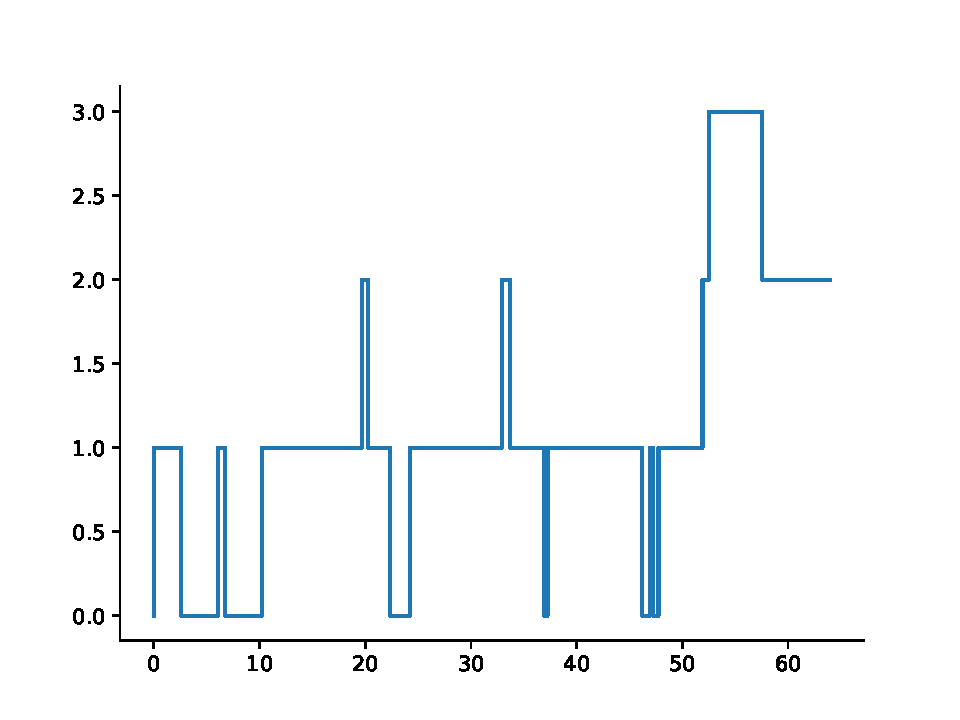
\includegraphics[width = 0.6\textwidth]{../Figures/traj_registration.pdf}
\caption{Un exemple de trajectoire du processus $X$}
\label{fig:traj_registration}
\end{figure}


\end{ex}
\section{Le générateur infinitésimal}
Eu égard aux équation de Chapman-Kolmogorov (\cf \cref{prop:CK}), nous avons que 
$$
P_t = (P_{t/n})^n,
$$
ainsi $P_t$ est entièrement déterminé par son comportement sur un intervalle de temps infinitésimal. Sa dérivée à droite est appelé générateur infinitésimal. On note que 
$$
p_0(x,y) = \begin{cases}
1,&\text{ si }x=y,\\
0,& \text{ sinon.}
\end{cases}
$$ 
\begin{theo}\label{theo:infinitesimal_generator}
Si $X$ est un processus de Markov à saut, il existe une matrice $Q$ telle que 
\begin{enumerate}
	\item $q(x,y)\geq 0$ pour tous $x,y\in E$ tels que $x\neq y$, et 
	$$
	q(x,x) = -\sum_{y\in E}q(x,y)
	$$
	\item Si $x\neq y$, $p_h(x,y) = hq(x,y) + o(h)$ et $p_h(x,x) = 1 + hq(x,x) + o(h)$
\end{enumerate}
\end{theo}
\begin{proof}
L'étude de $h\mapsto p_h(x,y)$ au voisinage de $0$ est lié à la loi du couple $(T_1, Z_1)$, où $T_1$ est le premier instant de saut de $X$ et $Z_1 = X_{T_1}$ l'état atteint après le saut. Pour un évènement $A$ et $x\in E$, on note 
$$
\Prob_x(A) = \Prob(A|X_0  = x).
$$
\begin{lemma}\label{lem:T_Z}
Soit $h,t>0$ et $m:=m(h,t)\in \N$ tel que $mh\downarrow t$ lorsque $h\downarrow0$. (par exemple $m = \lfloor t/h\rfloor+1$). Alors pour $x\neq y$, on a les deux limites suivantes
$$
\Prob_x( T_1>t) = \underset{h\downarrow 0}{\lim} p_h(x,x)^m
,\text{ et }\Prob_x(T_1\leq t, Z_1 = y) = \underset{h\downarrow0}{\lim}\frac{1-p_h(x,x)^m}{1-p_h(x,x)}p_h(x,y)
$$
\end{lemma}
\begin{proof}
Tout évènement $B$ satisfait 
\begin{equation}\label{eq:dummy_inclusion}
B\subset(B\cap\{T_2-T_1 > h\})\cup\{T_2 - T_1 \leq h\}.
\end{equation}
Nous avons l'inclusion suivante 
$$
\{T_1 >mh\}\subset B = \{X_0 = X_{h} = \ldots, X_{mh}\}\subset\{T_1>mh\}\cup \{T_2 - T_1\leq h\}.
$$
La première inclusion est évidente. Pour la deuxième, on utilise \eqref{eq:dummy_inclusion}. On note que pour $\omega\in B\cap\{T_2-T_1 > h\}$, on ne peut avoir $T_1(\omega)\leq mh$ car sinon on aurait un saut pendant un intervalle de longueur inférieure à $h$\footnote{Faire un schéma.}. On en déduit que $B\cap\{T_2-T_1>h\}\subset\{T_1 > mh\}$ Comme $\underset{h\downarrow 0}{\lim}\Prob_x(T_2 - T_1\leq h) = \Prob(T_2 = T_1) = 0$ alors 
\begin{eqnarray*}
\Prob_x(T_1>t) &=&\underset{h\downarrow 0}{\lim}\Prob_x(T_1>mh)\\
&=&\underset{h\downarrow 0}{\lim}\Prob_x(X_0 = X_h = \ldots = X_{mh})\\
&=&\underset{h\downarrow 0}{\lim}p_h(x,x)^m\\
\end{eqnarray*}
Pour la deuxième limite, on pose 
$$
A = \bigcup_{l = 1}^m\{X_0 = X_h = \ldots, X_{(l-1)h} = x,X_{lh}=y\}
$$ 
On a les inclusions
$$
A\subset\{X_0 = x,Z_1 = y, T_1\leq mh\}\cup\{T_2-T_1 \le h\}
$$
et
$$
\{X_0 = x,Z_1 = y, T_1\leq mh\}\subset A\cup\{T_2-T_1 \le h\}
$$ 
par le même raisonnement que précédemment. On en déduit que 
\begin{eqnarray*}
\Prob_x(T_1\leq t, Z_1 = y)&=&\underset{h\downarrow 0}{\lim} \Prob_x(T_1\leq mh, Z_1 = y)\\
&=&\underset{h\downarrow 0}{\lim} \Prob_x(A)\\
&=&\underset{h\downarrow 0}{\lim}\sum_{l =1}^m \Prob(X_0 = X_h = \ldots= X_{(l-1)h} = s,X_{lh} = y)\\
&=&\underset{h\downarrow 0}{\lim}\sum_{l =1}^m p_h(x,x)^{l-1} p_h(x,y)\\
&=&\underset{h\downarrow 0}{\lim}\frac{1-p_h(x,x)^m}{1-p_h(x,x)} p_h(x,y)\\
\end{eqnarray*}
\end{proof}
En conservant les notations du lemme, 
$$
\ln \Prob_x(T_1>t) = \underset{h\downarrow}{\lim}\,m\ln p_h(x,x) <0.
$$
Comme $\underset{h\downarrow 0}{\lim} p_h(x,x) =1$ alors on a les équivalent suivant 
$$
\frac{\ln \Prob_x(T_1 > t )}{t}\sim \frac{hm\ln p_h(x,x)}{th}\sim \frac{\ln p_h(x,x)}{h}\sim \frac{p_h(x,x) - 1}{h}.
$$
Le quotient $\frac{p_h(x,x) - 1}{h}$ a une limite noté $- q_x$ avec $q_x = -\frac{\ln\Prob_x(T_1>t)}{t}\geq 0$. En posant $q(x,x)=-q_x$, on a bien le dévellopement limité 
$$
p_h(x,x) = 1 + hq(x,x) + o(h).
$$
D'après le \cref{lem:T_Z},
$$
\Prob_x(T_1\leq t, Z_1 = y) = \underset{h\downarrow0}{\lim} h\frac{1-p_h(x,x)^m}{1-p_h(x,x)}\frac{p_h(x,y)}{h}.
$$
On a 
$$
\underset{h\downarrow0}{\lim} \frac{h}{1-p_h(x,x)} = \frac 1q_x
$$
et
$$
\underset{h\downarrow0}{\lim} 1-p_h(x,x)^m =\underset{h\downarrow0}{\lim} 1-\e^{m\ln p_h(x,x)} =1-\e^{\ln \Prob_x (T_1 >t)}=1-\e^{-q_x t}.
$$ 
On en déduit que $\frac{p_h(x,y)}{h}$ admet une limite pour $h\rightarrow 0$ que l'on note $q(x,y)$. On a donc
$$
\Prob_x(T_1\leq t, Z_1 = y) = \frac{(1-\e^{-q_x t})q(x,y)}{q_x}.
$$
En sommant pour $y\neq x$, il vient 
$$
\Prob_x(T_1\leq t) = \frac{(1-\e^{-q_x t})\sum_{y\neq x}q(x,y)}{q_x}.
$$
Comme $\Prob_x(T_1> t) = \e^{-q_x t }$ alors nécéssairement $\sum_{y\neq x}q(x,y)= q_x = -q(x,x)$ ce qui complète la preuve.
\end{proof}
\begin{ex}
\begin{enumerate}
	\item Le générateur infinitésimal associé à un processus de Poisson d'intensité $\lambda$ est donnée par
	$$
Q = \left(
\begin{array}{cccccc}
-\lambda&\lambda&0&0&\cdots&0\\
0&-\lambda&\lambda&0&\cdots&0\\
0&0&\ddots&\ddots&\cdots&0\\
\vdots&\vdots&\vdots&\ddots&\ddots&\vdots\\
0&0&0& 0&\cdots&\vdots
\end{array}
\right).
$$ 
Le graph des transitions est donné par la \cref{fig:transition_Poisson}.
\begin{figure}[h!]
\begin{center}
\begin{tikzpicture}[->, >=stealth', auto, semithick, node distance=3cm]
\tikzstyle{every state}=[fill=white,draw=black,thick,text=black,scale=0.8]
\node[state]    (1)                     {$0$};
\node[state]    (2)[right of = 1]                     {$1$};
\node[state]    (3)[right of = 2]                     {$2$};
\node[state]    (4)[right of=3]   {$\ldots$};
\path
(1) edge[left, above]    node{$\lambda$} (2)
(2) edge[left, above]    node{$\lambda$} (3)
(3) edge[left, above]    node{$\lambda$} (4)

% (2) edge[bend left]    node{$5/9$} (3)
% (3) edge[bend left]    node{$4/9$} (2)
% (3) edge[bend left]    node{$5/9$} (4)
% (4) edge[bend left]    node{$4/9$} (3)
% (4) edge[bend left]    node{$5/9$} (5)
% (5) edge[bend left]    node{$1$} (4)
;
\end{tikzpicture}
\end{center}
\caption{Graph des transitions pour le processus de Poisson.}
\label{fig:transition_Poisson}
\end{figure}
\item Le générateur de la file d'attente vu dans l'\cref{ex:registration} est donnée par 
	$$
Q = \left(
\begin{array}{ccccc}
-1/4&1/4&0&0&0\\
1/5&-9/20&1/4&0&0\\
0&1/5&-9/20&1/4&0\\
0&0&1/5&-9/20&1/4\\
0&0&0&1/5&-1/5\\
\end{array}
\right).
$$ 
Le graph des transitions est donné par la \cref{fig:transition_Poisson}.
\begin{figure}[h!]
\begin{center}
\begin{tikzpicture}[->, >=stealth', auto, semithick, node distance=3cm]
\tikzstyle{every state}=[fill=white,draw=black,thick,text=black,scale=0.8]
\node[state]    (1)                     {$0$};
\node[state]    (2)[right of = 1]                     {$1$};
\node[state]    (3)[right of = 2]                     {$2$};
\node[state]    (4)[right of=3]   {$3$};
\node[state]    (5)[right of=4]   {$4$};
\path
(1) edge[bend left, above]    node{$1/4$} (2)
(2) edge[bend left, above]    node{$1/5$} (1)
(2) edge[bend left, above]    node{$1/4$} (3)
(3) edge[bend left, above]    node{$1/5$} (2)
(3) edge[bend left, above]    node{$1/4$} (4)
(4) edge[bend left, above]    node{$1/5$} (3)
(4) edge[bend left, above]    node{$1/4$} (5)
(5) edge[bend left, above]    node{$1/5$} (4)

% (2) edge[bend left]    node{$5/9$} (3)
% (3) edge[bend left]    node{$4/9$} (2)
% (3) edge[bend left]    node{$5/9$} (4)
% (4) edge[bend left]    node{$4/9$} (3)
% (4) edge[bend left]    node{$5/9$} (5)
% (5) edge[bend left]    node{$1$} (4)
;
\end{tikzpicture}
\end{center}
\caption{Graph des transitions pour le processus d'inscription à l'université.}
\label{fig:transition_queue}
\end{figure}
\end{enumerate}

\end{ex}

\begin{prop}
Soit un processus de Markov $X$ de générateur infinitésimal $Q$ et de matrice des transitions $(P_t)_{t\geq0}$. Alors on a 
\begin{itemize}
	\item L'équation progressive ou \textit{forward}
	$$
	P_t' = P_t Q.
	$$
	\item L'équation rétrograde ou \textit{backward}
	$$
	P_t' = Q P_t.
	$$
\end{itemize}
\end{prop}
\begin{proof}
Il s'agit d'une conséquence des équation de Chapman-Kolmogorov et du \cref{theo:infinitesimal_generator}. Pour l'équation progressive, avec $h,t>0$, on a 
\begin{eqnarray*}
\frac{P_{t+h} - P_t}{h}&=&\frac{P_{t}P_{h} - P_t}{h}\\
&=&P_t\left(\frac{P_{h} - I}{h}\right)\\
&=&P_t\left(\frac{P_{h} - P_0}{h}\right)\\
\end{eqnarray*}
En passant à la limite pour $h\rightarrow 0$, il vient $P_t' = P_tQ$.
\end{proof}
\begin{ex}[Processus à deux états]\label{ex:two_state_cont_markov_chain}
Soit un processus de Makov $X$ sur $E=\{1, 2\}$ caractérisé par son générateur infinitésimal 
$$
Q = \left(\begin{array}{cc}
-\lambda & \lambda\\
\mu & -\mu
\end{array}\right)
$$
Trouver la matrice des transitions $P_t$ revient à résoudre un système d'équation différentielle. On a par exemple
\begin{eqnarray*}
p_t(1,1)' &=& -\lambda p_t(1,1)+ \mu[1- p_t(1,1)]\\
&=& \mu - (\lambda + \mu)p_t(1,1)
\end{eqnarray*}
Avec la condition $p_0(1,1) = 1$, on a 
$$
p_t(1,1) = \frac{\mu}{\lambda + \mu} + \frac{\lambda}{\lambda + \mu}\e^{-(\lambda + \mu)t}.
$$
On peut effectuer les mêmes calculs pour $p_t(1,2)$, $p_t(1,2)$ et $p_t(2,2)$. On obtient finalement
$$
P_t = \frac{1}{\lambda + \mu}
\left(\begin{array}{cc}
\mu +\lambda \e^{-(\lambda +\mu)t}&\lambda -\lambda \e^{-(\lambda +\mu)t}\\
\mu -\mu \e^{-(\lambda +\mu)t}&\lambda +\mu \e^{-(\lambda +\mu)t}\\
\end{array}\right).
$$
\end{ex}
Plus généralement, le lien entre la matrice des transitions $P_t$ et le générateur $Q$ s'exprime au moyen l'opérateur exponentiel pour les matrice. 
\begin{prop}
On a 
$$
P_t = \e^{tQ} = \sum_{n=0}^\infty\frac{(tQ)^n}{n!}.
$$
\end{prop} 
On rappelle que l'opérateur exponentiel pour les matrices vérifie les propriété suivantes:
\begin{enumerate}
	\item $\e^0 = I$
	\item $\e^A\e^{-A} = I$
	\item $\e^{(s+t)A} = \e^{sA}\e^{tA}$
	\item Si $AB = BA$ alors $\e^{A+B}=\e^{A}\e^{B}=\e^{B}\e^{A}$
	\item $\frac{\text{d}}{\text{d}t}\e^{tA} = A\e^{tA} = \e^{tA}A$
\end{enumerate}
pour $A,B\in M_n(\RL)$ et $s,t\geq0$. On peut facilement calculer l'exponentielle d'une matrice en python, à la main il faut diagonaliser la matrice $Q$ (sous réserve que celle ci soit diagonalisable).
\begin{ex}\label{ex:two_state_exp}
On reprend l'\cref{ex:two_state_cont_markov_chain}. La matrice 
$$
Q = \left(\begin{array}{cc}
-\lambda & \lambda\\
\mu & -\mu
\end{array}\right)
$$
est diagonalisable. Elle admet pour valeur propre $0$ et $-(\lambda + \mu)$, les vecteurs propres asssociés sont 
$$
\left(\begin{array}{c} 1\\
1\end{array}\right)\text{, et } \left(\begin{array}{c} -\lambda\\
\mu\end{array}\right).
$$
On obtient la décomposition
$$
Q = S D S^{-1} = \left(\begin{array}{cc}
1& -\lambda\\
1 & \mu
\end{array}\right)\left(\begin{array}{cc}
0& 0\\
0 & -(\lambda +\mu)
\end{array}\right)\left(\begin{array}{cc}
\mu/(\lambda + \mu) & \lambda/(\lambda + \mu)\\
-1/(\lambda + \mu)& 1/(\lambda + \mu)
\end{array}\right).
$$
Cela permet d'exprimer la matrice des transition par 
\begin{eqnarray*}
P_t &=& \e^{tQ}\\
 &=& S\e^{tD}S^{-1}\\ 
 &=& \left(\begin{array}{cc}
1& -\lambda\\
1 & \mu
\end{array}\right)\left(\begin{array}{cc}
1& 0\\
0 & \e^{-(\lambda +\mu)}
\end{array}\right)\left(\begin{array}{cc}
\mu/(\lambda + \mu) & \lambda/(\lambda + \mu)\\
-1/(\lambda + \mu)& 1/(\lambda + \mu)
\end{array}\right) \\
&=& \frac{1}{\lambda + \mu}
\left(\begin{array}{cc}
\mu +\lambda \e^{-(\lambda +\mu)t}&\lambda -\lambda \e^{-(\lambda +\mu)t}\\
\mu -\mu \e^{-(\lambda +\mu)t}&\lambda +\mu \e^{-(\lambda +\mu)t}\\
\end{array}\right).
\end{eqnarray*}
\end{ex}
\section{Comportement asymptotique}\label{sec:asymptotic_behavior}
Le comportement asymptotique d'une chaine de Markov en temps continu est similaire à celui d'une chaine de Markov en temps discret. Si la chaine de Markov possède les propriété d'irréductibilité et de récurrence alors il existe une unique loi invariante qui jouera le rôle de loi stationnaire. Soit $X=(X_t)_{t\geq 0}$ un processus de Markov sur $E$ de générateur $Q$ et de matrice des transition $t\mapsto P_t$.
\begin{definition}
Une loi de probabilité $\pi = (\pi(x))_{x\in E}$ sur $E$ est la loi stationnaire de $X$ si 
$$
\underset{t\rightarrow \infty}{\lim} p_t(x,y) = \pi(y)
$$
\end{definition}
La loi stationnaire est toujours une loi invariante de $X$
\begin{definition}
Une loi de probabilité $\pi = (\pi(x))_{x\in E}$ sur $E$ est une loi invariante de $X$ si 
$$
\pi = \pi P_t,\text{ pour tout }t\geq0.
$$
De plus, on a également 
$$
\pi Q = 0.
$$
NB: $\pi$ est un vecteur ligne de dimension $\text{Card}(E)$.
\end{definition}
Si $\pi P_t = \pi$ alors $0 = \pi P_t' = \pi Q$. Inversement si $\pi Q = 0$ alors $\pi Q P_t = 0$, puis $\pi P_t' = 0$. On en déduit que $\pi P_t = \text{Cste} = \pi P_0  = \pi I =  \pi$.
\begin{theo}
Si $X$ est un processus de Markov irréductible sur un espace d'état fini alors il existe une unique loi invariante qui est aussi la loi stationnaire.
\end{theo}
\begin{ex}
On reprend le processus des exemples \ref{ex:two_state_cont_markov_chain} et \ref{ex:two_state_exp}. On note que $\pi = \left(\begin{array}{cc}\frac{\mu}{\lambda +\mu} & \frac{\lambda}{\lambda +\mu}\end{array}\right)$ vérifie  
$$
\pi Q = 0\text{, et }\pi \,^t\mathbf{1}_2 = 1, 
$$
où $\mathbf{1}_2 = \left(\begin{array}{cc}1&1\end{array}\right)$, et que 
\begin{equation}\label{eq:transition_matrix_subordinated_poisson}
P_t = 
\left(\begin{array}{cc}
\mu +\lambda \e^{-(\lambda +\mu)t}&\lambda -\lambda \e^{-(\lambda +\mu)t}\\
\mu -\mu \e^{-(\lambda +\mu)t}&\lambda +\mu \e^{-(\lambda +\mu)t}\\
\end{array}\right)
\rightarrow
\left(\begin{array}{cc}
\mu / (\lambda + \mu)&\lambda/(\lambda + \mu)\\
\mu /(\lambda + \mu)&\lambda/(\lambda + \mu)\\
\end{array}\right)\text{ pour }t\rightarrow \infty.
\end{equation}
\end{ex}
La loi stationnaire s'interprête comme le temps moyen passé dans chaque état par le processus $X$ dans le cadre d'une trajectoire de longueur infini. Lorsque l'espace d'état est infini alors l'étude du comportement asymptotique nécessite d'introduire la notion d'état récurrent et transitoire. On note
$$
R_x =\inf\{t>T_1\text{ ; }X_t = x\}
$$ 
le temps de premier retour à l'état $x$ (sous entendu $X_0 = x$).
\begin{definition}\label{def:recuurent_state}
Un état $x\in E$ 
\begin{itemize}
    \item est récurrent si 
    $$
    \Prob_x(R_x<\infty) = 1, 
    $$
    de plus $x$ est 
    \begin{itemize}
        \item récurrent positif si $\E_x(R_x) <\infty $
        \item récurrent nul si $\E_x(R_x) =\infty $
    \end{itemize}
    \item est transitoire si 
    $$
    \Prob_x(R_x = \infty) > 0. 
    $$
\end{itemize}
\end{definition}
\begin{theo}
La loi stationnaire de $X$ existe et est unique si $X$ est irréductible et que tous les états sont récurrents positifs. 
\end{theo}
\begin{proof}
admis
\end{proof}
\begin{remark}
Ces notions sont aussi valables pour les chaines de Markov en temps discret. Si les propriétés de récurrence sont vérifiées pour la chaine de Markov immergé
$$
Z_n = X_{T_{n}},\text{ }n\geq 0,
$$
où les $T_n$ sont les instants de saut, alors elles sont vérifiées pour le processus $X$ et vice-versa. Ces notions sont abordées dans mes notes de cours sur les chaines de Markov \url{http://pierre-olivier.goffard.me/mad/}.
\end{remark}
Si l'espace d'état est infini, il est hors de question de résoudre un système linéaire. Il est plus facile de trouver une loi réversible
\begin{definition}
Une loi $\lambda$ sur $E$ est dite réversible si elle vérifie
$$
\lambda(x)q(x,y)= \lambda(y)q(y,x), \text{ pour tout }(x,y)\in E.
$$
\end{definition}
\begin{prop}
Soit $\lambda$ une loi sur $E$, alors 
$$
\lambda\text{ réversible}\Rightarrow \lambda\text{ invariante}.
$$
\end{prop}
\begin{proof}
\begin{eqnarray*}
\lambda Q &=& \left(\begin{array}{ccc}\sum_{x\in E}\lambda(x)q(x,y_1)&\sum_{x\in E}\lambda(x)q(x,y_2)&\cdots\end{array}\right) \\
&=&\left(\begin{array}{ccc}\sum_{x\in E}\lambda(y_1)q(y_1,x)&\sum_{x\in E}\lambda(y_2)q(y_2,x)&\cdots\end{array}\right)\\
 &=& \left(\begin{array}{ccc}0&0&\cdots\end{array}\right).
\end{eqnarray*}
\end{proof}
\begin{remark}
Si $X$ admet une loi stationnaire réversible alors le processus est réversible dans le temps. Sur le long terme, on ne fait pas la différence entre les processus $X_t$ et $X_{T-t}$.
\end{remark}

\section{Processus de naissance-mort}
Les processus de naissance-mort sont des processus de Markov $X = (X_t)_{t\geq 0}$ tels que 
$$
Q=\left(
\begin{array}{ccccccc}
-\lambda_0&\lambda_0&0&0&0&\cdots \\
\mu_1&-(\mu_1 +\lambda_1)&\lambda_1&0&0&\cdots \\
0&\mu_2&-(\mu_2 +\lambda_2)&\lambda_2&0&\cdots \\
0&0&\ddots&\ddots&\ddots &\vdots \\
\vdots&\vdots&\vdots&\vdots&\vdots&\vdots
\end{array}
\right).
$$
\begin{ex}
Le processus de Poisson est un processus de naissance dont les taux de naissance sont constants, égaux à l'intensité de processus.
\end{ex}
Pour étudier la loi stationnaire du processus de naissance-mort, on recherche une loi $\pi$ réversible. Elle vérifie 
$$
\pi(x)\lambda_{x} = \pi(x+1)\mu_{x+1},\text{pour tout }x \geq0.
$$
On en déduit que 
$$
\pi(x) = \pi(0)\prod_{k=1}^x\frac{\lambda_{k-1}}{\mu_k}.
$$
On en déduit l'existence d'une loi réversible si 
$$
S = \sum_{x=1}^{\infty}\prod_{k=1}^x\frac{\lambda_{k-1}}{\mu_k} <\infty,
$$
auquel cas 
$$
\pi(0) = (1+S)^{-1}.
$$
L'unicité est plus difficile à montrer. Voyons un exemple en théorie des files d'attente. 
\section{Théorie des files d'attente et loi de Little}
Soit un système comprenant des clients et des serveurs, caractérisé par trois paramètres
\begin{enumerate}
    \item La fréquence d'arrivée des clients
    \item Le temps de service par un serveur
    \item le nombre de serveurs 
\end{enumerate}
On définit un processus $X = (X_t)_{t\geq 0}$ qui modélise le nombre de client dans le système. En supposant que le processus converge vers une loi stationnaire alors on a la relation suivante (merci à \citet{Little1961}).
\begin{theo}
$$L = \lambda W,$$
avec 
\begin{itemize}
    \item $L$ le nombre de clients moyen lorsque $t\rightarrow \infty$
    \item $\lambda$ le nombre moyen de client qui arrive par unité de temps
    \item $W$ le temps moyen d'attente d'un client dans le système lorsque $t\rightarrow \infty$
\end{itemize}
\end{theo}
\begin{proof}
Il s'agit plus d'une intuition qu'une preuve rigoureuse (voir \citet{Little1961} pour la preuve) . Soit $(N_t)_{t\geq0}$ le processus qui compte le nombre de client entrés dans le système. Soit $T_1,\ldots, T_{N_t}$ les temps d'arrivée des clients. On note $S_1,\ldots, S_{N_t}$ les temps de sortie du système des clients. On considère une trajectoire du processus $X$ entre $[0, t]$ tel que $S_{N_t} = t$ et $T_{N_t+1}>t$. Un exemple d'une telle trajectoire est donnée par la \cref{fig:queue_little}.
\begin{figure}[ht!]
\begin{center}
\begin{tikzpicture}
  %Origin and axis
  \coordinate (O) at (0,0);
  \draw[->] (-1,0) -- (9,0) coordinate[label = {below:$$}] (xmax);
  \draw[->] (0,-0.5) -- (0,3) coordinate[label = {left:$X_t$}] (ymax);
  %Lower linear boundary

 
  %Stochastic process trajectory
  
  \draw (0,0) node[blue,left] {} node{};
  \draw[very thick,blue,-] (0,0) -- (0.5,0) node[pos=0.5, above] {} ;
  \draw[very thick,blue] (0.5,0) -- (0.5,1) node[pos=0.5, right] {};
  \draw[very thick,blue,-] (0.5, 1) -- (1.25,1) node[pos=0.5, above] {};
  \draw[very thick,blue] (1.25,1) -- (1.25,2) node[pos=0.5, right] {};
  \draw[very thick,blue,-] (1.25,2) -- (2,2) node[pos=0.5, above] {};
  \draw[very thick,blue] (2,2) -- (2,3) node[pos=0.5, right] {};
  \draw[very thick,blue] (2,3) -- (3,3) node[pos=0.5, right] {};
  \draw[very thick,blue] (3,3) -- (3,2) node[pos=0.5, right] {};
  \draw[very thick,blue,-] (3,2) -- (3.4,2)node[pos=0.5, above] {};
  \draw[very thick,blue] (3.4,2) -- (3.4,1) node[pos=0.5, right] {};  
  \draw[very thick,blue,-] (3.4,1) -- (4,1) node[pos=0.5, above] {};
  \draw[very thick,blue] (4,1) -- (4,2) node[pos=0.5, right] {};  
  \draw[very thick,blue,-] (4,2) -- (6,2) node[pos=0.5, above] {};
  \draw[very thick,blue,-] (6,2) -- (6,1) node[pos=0.5, above] {};
   \draw[very thick,blue,-] (6,1) -- (8,1) node[pos=0.5, above] {};
    \draw[very thick,blue,-] (8,1) -- (8,0) node[pos=0.5, above] {};
     % \draw[very thick,blue,-] (,0.5) -- (8,0.5) node[pos=0.5, above] {};
     % \draw[very thick,blue,-] (8,0.5) -- (8,0) node[pos=0.5, above] {};
  %Jump Times
  \draw (0.5,0) node[black,below] {$T_1$} node{ \color{black}$\bullet$};
  \draw (1.25,0) node[black,below] {$T_2$} node{ \color{black}$\bullet$};
  \draw (2,0) node[black,below] {$T_3$} node{ \color{black}$\bullet$};
  \draw (3,0) node[black,below] {$S_1$} node{ \color{black}$\bullet$};
  \draw (3.4,0) node[black,below] {$S_2$} node{ \color{black}$\bullet$};
  \draw (4,0) node[black,below] {$T_4$} node{ \color{black}$\bullet$};
  \draw (6,0) node[black,below] {$S_3$} node{ \color{black}$\bullet$};
  \draw (8,0) node[black,below] {$S_4 =t$} node{ \color{black}$\bullet$};
  %Level of the counting process
   \draw (0,0) node[black,below left] {$0$} node{};
   % \draw (0,0.5) node[black,left] {$1$} node{ \color{black}$-$};
   % \draw (0,1) node[black,left] {$2$} node{ \color{black}$-$};
   % \draw (0,1.5) node[black,left] {$3$} node{ \color{black}$-$};
   % \draw (0,2) node[black,left] {$4$} node{ \color{black}$-$};
   % \draw (0,2.5) node[black,left] {$5$} node{ \color{black}$-$};

  % %Aggregated Capital gains
%  \draw (0,1.5) node[blue,below right] {$\mu_1$} node{ \color{blue}$-$};
%  \draw (0,2.25) node[blue,left] {$\mu_2$} node{ \color{blue}$-$};
%  \draw (0,3.75) node[blue,left] {$\mu_3$} node{ \color{blue}$-$};
  %Ruin time = First-crossing time time
%  \draw (5,0) node[black,above right] {${\tau_0}_u$} node{ \color{black}$\times$};
%  \draw[dotted,black] (0,3.28) -- (5,3.28);
%  \draw[dotted,black] (5,0) -- (5,3.28);
\end{tikzpicture}
\end{center}
\caption{Trajectoire du processus $X_t$ tel que $N_t = 4$.}
\label{fig:queue_little}
\end{figure}
La preuve consiste à calculer l'aire sous la courbe $A$ de deux façons. On a d'une part,
\begin{eqnarray*}
W &=& \frac{1}{N_t}\sum_{i=1}^{N_t}(S_i - T_i)\\
&=& \frac{(S_1 - T_1) + (S_2 - T_2) + (S_3-T_3) - (S_4-T_4)}{4}\\
&=&\frac{(S_4 - T_1) + (S_3 - T_4) + (S_2-T_2) + (S_1-T_3)}{4}\\
&=&\frac{A}{N_t}.
\end{eqnarray*}
On a d'autre part
\begin{eqnarray*}
L &=& \frac{1}{t}\int_0^t X_s\text{d}s\\
&=&\frac{1\cdot(T_2-T_1) + 2\cdot(T_3-T_2) + 3\cdot(T_3-S_1)+ 2\cdot(S_1-S_2) + 1\cdot(S_2 - T_4) + 2\cdot(T_4 - S_3) - 1\cdot(S_4 - S_3)}{t}\\
&=&\frac{A}{t}.
\end{eqnarray*}
On en déduit que 
$$
L = \frac{N_t}{t}W\rightarrow L = \lambda W.
$$
\end{proof}
Cette loi est très utile en pratique car on a parfois accès à $W$ facilement mais pas à $L$ ou inversement. On répond alors à des questions du type 
\begin{itemize}
	\item Quel est la longueur moyenne de la file d'attente?
	\item Si je vais au magasin, quel est mon temps d'attente moyen avant que le service commence?
	\item Quel est le temps moyen passé par un client dans le système?
\end{itemize}
\begin{ex}[file d'attente M/M/1 queue]
Supposons que le nombre de client arrivant dans le système est gouverné par un processus de Poisson d'intensité $\lambda$. Supposons ces unités sont servis par un unique serveur et que le temps de service soit une loi exponentielle de paramètre $\mu$. Le nombre de client dans le système est modélisé par un processus $X$. Ce processus est une file d'attente du type $M/M/1$ où $M$ signifie \textit{memoryless}. Le générateur du processus est donnée par 
$$
Q=\left(
\begin{array}{ccccccc}
-\lambda&\lambda&0&0&0&\cdots \\
\mu&-(\mu +\lambda)&\lambda&0&0&\cdots \\
0&\mu&-(\mu +\lambda)&\lambda&0&\cdots \\
0&0&\ddots&\ddots&\ddots &\vdots \\
\vdots&\vdots&\vdots&\vdots&\vdots&\vdots
\end{array}
\right).
$$
Il s'agit d'un processus de naissance mort dont les taux de naissance et de mort sont constants. La loi stationnaire existe si 
$$
S = \sum_{x = 1}^\infty\left(\frac{\lambda}{\mu}\right)^x <\infty,
$$
cela équivaut à $\lambda <\mu$ avec 
$$
S = \frac{\lambda}{\mu}\left(\frac{1}{1-\lambda / \mu}\right).
$$
On en déduit la loi stationaire du processus 
$$
\pi(x) = \left(1-\frac{\lambda}{\mu}\right)\left(\frac \lambda\mu\right)^x,\text{ pour }x\geq 0.
$$
Il s'agit d'une loi géométrique de paramètre $1-\lambda / \mu$. Le nombre moyen de clients dans le système est donc 
$$
L = \frac{\lambda}{\lambda - \mu}
$$
On en déduit le temps moyen passé dans le système via la loi de Little avec 
$$
W = \frac{L}{\lambda} = \frac{1}{\lambda - \mu}
$$
On peut considérer que la file d'attente comprend tous les client du système sauf celui en train d'être servi. Le temps moyen passé $W_q$ dans la file d'attente est donné par
$$
W_q = W - W_s, 
$$
où $W_s$ est le temps de service moyen. Il vient 
$$
W_q= \frac{\lambda}{\mu(\mu - \lambda)}.
$$
La longueur moyenne $L_q$ de la file d'attente peut être déterminé par la loi de Little en restreignant le système à la file d'attente. Il vient 
$$
L_q = \lambda W_q = \frac{\lambda^2}{\mu(\mu - \lambda)}.
$$


\end{ex}
De manière générale, un processus de type file d'attente atteint la stationarité lorsque les sorties du système dominent les entrées.
\section{Chaine de Markov subordonnée à un processus de Poisson}\label{sec:subordinated_poisson}
Soit $Y=(Y_n)_{n\geq 0}$ une chaine de Markov de matrice des transition $A$ sur un espace d'état $E$. On peut construire un processus de markov à partir de $Y$ et d'un processus de Poisson $N = (N_t)_{t\geq 0}$ d'intensité $\lambda$, indépendant de $Y$.
\begin{prop}\label{prop:subordinated_poisson}
Le processus défini par 
$$
X_t = Y_{N_t},\text{ }t\geq 0,
$$
est un processus de Markov de matrice des transitions données par 
$$
P_t = \exp[\lambda t(A - I)].
$$
\end{prop}
\begin{proof}
Soit $x,y \in E$
\begin{eqnarray*}
p_t(x,y) &=& \Prob(X_t = y|X_0 = x)\\
&=&\sum_{k=0}^\infty\Prob(X_t = y|X_0 = x, N_t = k)\Prob(N_t = k)\\
&=&\sum_{k=0}^\infty\Prob(Y_k = y|Y_0 = x)\frac{(\lambda t)^k\e^{-\lambda t} }{k!}\\
&=&\sum_{k=0}^\infty A^k_{x,y}\frac{(\lambda t)^k\e^{-\lambda t} }{k!}.
\end{eqnarray*}
On peut vérifier que c'est bien équivalent à \eqref{eq:transition_matrix_subordinated_poisson}. En effet, 
\begin{eqnarray*}
\exp[\lambda t(A - I)]&=& \sum_{k=0}^\infty\frac{(\lambda t^k}{k!}(A-I)^k\\
&=&\sum_{k=0}^\infty\frac{(\lambda t^k}{k!}\sum_{l=0}^k\binom{k}{l}A^l(-1)^{k-l}\\
&=&\sum_{k=0}^\infty\sum_{l=0}^k\frac{(\lambda t^k}{l!(k-l)!}A^l(-1)^{k-l}\\
&=&\sum_{l=0}^\infty\sum_{k=l}^\infty\frac{(\lambda t^k}{l!(k-l)!}A^l(-1)^{k-l}\\
&=&\sum_{l=0}^\infty \frac{A^l}{l!}\sum_{k=l}^\infty\frac{(\lambda t)^k}{(k-l)!}(-1)^{k-l}\\
&=&\sum_{l=0}^\infty A^l\frac{(\lambda t)^l}{l!}\e^{-\lambda t}\\
\end{eqnarray*}
Pour compléter la preuve on vérifie que pour $0= t_0<t_1<\ldots, t_n$ des instants et $x_0, x_1,\ldots, x_n$ des états de $E$, on a 
$$
\Prob(X_{t_0} = x_0, X_{t_1} = x_1,\ldots, X_{t_n}=x_n) = P_{t_1}(x_0,x_1)\ldots P_{t_n - t_{n-1}}(x_{n-1}, x_n).
$$
Il faut conditionner par rapport au valeur du processus $N$ aux temps $t_1,\ldots, t_n$ et c'est un peu fastidieux à écrire.
\end{proof} 
On peut identifier le générateur de $X$ par
$$
Q = \lambda(A-I).
$$
Inversement à partir d'un processus de Markov $X$ dont les temps de séjour sont bornées, $q_x <\lambda$ pour tout $x\in E$, on observe que 
$$
A = \frac{Q}{\lambda} + I
$$
est une matrice stochastique\footnote{Tous les coefficients sont positifs et les lignes se somment à $1$.}. Il ne faut toutefois pas confondre la chaine $Y$ de matrice des transition $A$ avec la chaine immergée Z définie plus haut!

\section{Loi \textit{phase-type}}\label{sec:phase_type}
Soit une processus de Markov $X=(X_t)_{t\geq 0}$ sur un espace d'état $E\cup\{\dagger\}$ comprenant un état absorbant caractérisés par un temps de séjour infini, soit
$$
q_\dag = 0.
$$
Le générateur de $X$ s'écrit alors par bloc avec 
$$
Q = \left(\begin{array}{c|c}
T&t\\
\hline
0&0
\end{array}\right),
$$
où $t$ et $T$ sont respectivement des vecteur et matrice carré de dimension $\text{Card}(E)$, tel que $t  + T \mathbf{1}_E = 0$, où $\mathbf{1}_E$ est un vecteur ne contenant que des $1$. Le vecteur $t$ correspond aux taux de transition vers l'état absorbant (les taux d'absorbtion) depuis chacun des état de $E$. Le temps d'absorbtion 
$$
\tau = \inf\{t\geq 0\text{ ; }X_t =\dagger\},
$$
suit une loi \textit{phase-type}, noté $\text{PH}(\alpha, T)$, où $\alpha$ est la loi initiale de $X$. Les lois $\textit{phase type}$ sont denses dans les lois de probabilité sur $\RL_+$\footnote{N'importe loi  sur $\RL_+$ peut s'écrire comme la limite d'une suite de loi \textit{phase type}.}. De nombreuses lois usuelles sont des cas particuliers de loi \textit{phase-type}.
\begin{ex}
\begin{enumerate}
	\item La loi $\ExpDist(\lambda)$ est une loi \textit{phase-type}, avec 
	$$
	\alpha = (\begin{array}{cc}1&0\end{array})\text{,  }Q = \left(\begin{array}{c|c}-\lambda & \lambda\\
	\hline
	0&0
	\end{array}\right).
	$$
    Schématiquement, 
\begin{center}
\begin{tikzpicture}[->, >=stealth', auto, semithick, node distance=3cm]
\tikzstyle{every state}=[fill=white,draw=black,thick,text=black,scale=0.8]
\node (0) {$$};
\node[state]    (1)[right of = 0]                     {$1$};
\node[state]    (2)[right of=1]   {$\dagger$};
\path
(0) edge[left, above]    node{$1$} (1)
(1) edge[left, above]    node{$\lambda$} (2)

% (2) edge[bend left]    node{$5/9$} (3)
% (3) edge[bend left]    node{$4/9$} (2)
% (3) edge[bend left]    node{$5/9$} (4)
% (4) edge[bend left]    node{$4/9$} (3)
% (4) edge[bend left]    node{$5/9$} (5)
% (5) edge[bend left]    node{$1$} (4)
;
\end{tikzpicture}
\end{center}
\item La loi $\GammaDist(k,\lambda)$, avec $k\in \mathbb{N}$, de densité 
$$
f(t) = \frac{\e^{\lambda t}\lambda^k t^{k-1}}{k!},\text{ pour }t>0,
$$
est une loi \textit{phase-type}, avec 
	$$
	\alpha = (\begin{array}{ccc}1& \cdots&0\end{array})\text{,  }
	Q = \left(
	\begin{array}{ccccc|c}
	-\lambda &\lambda&0&\cdots&0&0 \\
	0&-\lambda&\lambda&\cdots&0&0\\
	\vdots&0&\ddots&\ddots&\vdots&\vdots\\
	0&0&\cdots&0&-\lambda&\lambda\\
    \hline
    0&0&\cdots&0&0&0
	\end{array}
	\right).
	$$
    Schématiquement, 
\begin{center}
\begin{tikzpicture}[->, >=stealth', auto, semithick, node distance=3cm]
\tikzstyle{every state}=[fill=white,draw=black,thick,text=black,scale=0.8]
\node (0) {$$};
\node[state]    (1)[right of = 0]                     {$1$};
\node[state]    (2)[right of = 1]                     {$\cdots$};
\node[state]    (3)[right of = 2]                     {$k$};
\node[state]    (4)[right of=3]   {$\dagger$};
\path
(0) edge[left, above]    node{$1$} (1)
(1) edge[left, above]    node{$\lambda$} (2)
(2) edge[left, above]    node{$\lambda$} (3)
(3) edge[left, above]    node{$\lambda$} (4)

% (2) edge[bend left]    node{$5/9$} (3)
% (3) edge[bend left]    node{$4/9$} (2)
% (3) edge[bend left]    node{$5/9$} (4)
% (4) edge[bend left]    node{$4/9$} (3)
% (4) edge[bend left]    node{$5/9$} (5)
% (5) edge[bend left]    node{$1$} (4)
;
\end{tikzpicture}
\end{center}
\item La loi $\text{h-}\ExpDist(p,\lambda_1,\lambda_2)$, de densité 
$$
f(t) = p\lambda_1\e^{-\lambda_1 t} + (1 - p)\lambda_2\e^{-\lambda_2 t},\text{ pour }t>0.
$$
est une loi \textit{phase-type}, avec 
    $$
    \alpha = (\begin{array}{ccc}p& 1-p\end{array})\text{,  }
    Q = \left(
    \begin{array}{cc|c}
    -\lambda_1 &0&\lambda_1 \\
    0&-\lambda_2&\lambda_2\\
    \hline
    0&0&0
    \end{array}
    \right).
    $$
    Schématiquement, 
\begin{center}
\begin{tikzpicture}[->, >=stealth', auto, semithick, node distance=3cm]
\tikzstyle{every state}=[fill=white,draw=black,thick,text=black,scale=0.8]
\node (0) {$$};
\node (1)[right of = 0] {$$};
\node[state]   (2)[above of = 1] {$1$};
\node[state]    (3)[below of = 1] {$2$};
\node[state]    (4)[right of=1]   {$\dagger$};
\path
(0) edge[left, above]    node{$p$} (2)
(0) edge[left, below left]    node{$1-p$} (3)
(2) edge[left, above]    node{$\lambda_1$} (4)
(3) edge[left, below right]    node{$\lambda_2$} (4)

;
\end{tikzpicture}
\end{center}
\end{enumerate}
\end{ex}
Ces distributions donne une grande marche de manoeuvre à la modélisation. Leur représentation sous la forme de graph rend commode l'explication du modèles. On retrouve les lois \textit{phase type} dans de nombreux domaine d'application des probabilités. 
\begin{theo}
Soit $X$ une \va de loi $\text{PH}(\alpha, T)$, alors
\begin{enumerate}
    \item La fonction de répartition de $X$ est donnée par 
    $$
    F(x) = 1-\alpha\e^{Tx}\mathbf{1}_E
    $$
    \item La densité de $X$ est donnée par 
    $$
    f(x) = \alpha\e^{Tx}t
    $$
    \item L'espérance de $X$ est donnée par 
    $$
    \E(X) = -\alpha T^{-1}\mathbf{1}_E
    $$
    \item La fonction génératrice des moments $X$ est donnée par 
    $$
    M_X(\theta) = \E(\e^{\theta X}) = \alpha(-\theta I - T)^{-1}t
    $$
\end{enumerate}
\end{theo}
\begin{proof}
Voir \citet[Chapitre 9, Section 1]{Asmussen2010}
\end{proof}
En actuariat, les loi \textit{phase-type} sont utilisées pour
\begin{itemize}
    \item modéliser les montants de sinistres et le temps entre les sinistres, voir \citet{Bladt2005}, voir également la généralisation de \citet{Albrecher2019} pour permettre des distributions à queue lourdes
    \item modéliser la mortalité, voir \citet{Lin2007}
    \item modéliser l'entrée et le maintien en incapacité, voir \citet{Zadeh2013}
    \item valoriser des contrats de type épargne, voir\citet{Asmussen2019}
    \item tarifer via la théorie de la crédibilité, voir \citet{Zadeh2014}
\end{itemize}
L'estimation se fait par maximum de vraisemblance au moyen d'un algorithme d'espérance-maximisation (EM), voir \citet{Asmussen1996}. 
\begin{ex}
Le maintien en incapacité joue un rôle prépondérant en assurance emprunteur, et en prévoyance individuel. Les assurés ont généralement trois statuts
$$
\{\text{actif, incapable, décédé}\}
$$
qui peuvent former l'espace d'état $E$ d'un processus de Markov $X$ dont l'état absorbant est $\dagger = \text{décédé}$ et des aller-retours entre les états $\text{actif}$ et $\text{incapabale}$, comme sur la \cref{fig:transition_graph_disability}
\begin{figure}[!h]
 \begin{center}
\begin{tikzpicture}[->, >=stealth', auto, semithick, node distance=4cm]
% \tikzstyle{every state}=[fill=white,draw=black,thick,text=black,scale=0.8]
\tikzstyle{every state}=[rectangle,draw,rounded corners=4pt,fill=white]
\tikzstyle{test}=[diamond, aspect=2.5,thick, draw=blue,fill=yellow!50,text=blue] 

\node[test]    (1)               {$\text{Valide}$};
\node[test]    (2)[right of=1]   {$\text{Incapacité}$};
\node[state]    (3)[below right of=1]   {$\text{Décès}$};

\path
(1) edge[bend left] node[above]{} (2)
(2) edge[bend right] node[above]{} (1)
(1) edge[left]  node{} (3)
(2) edge[left]  node{} (3)
;
\end{tikzpicture}
\end{center}
\caption{Les états des assurés dans le cadre de la modélisation du maintien en incapacité}
\label{fig:transition_graph_disability}
\end{figure}
Le modèle  se complexifie en distinguant les différentes classes d'age $j=1\ldots, l$ associées à des taux d'entrée en incapacité distincts
$$
\beta_1,\ldots, \beta_l,
$$
des taux de retour à l'activité distincts
$$
\gamma_1,\ldots, \gamma_l,
$$
des taux de transitions de classes 
$$
\zeta_1,\ldots, \zeta_{l-1},
$$
et finalement des taux de décès distincts
$$
\delta_1,\ldots, \delta_l.
$$
Le modèle complet est donnée par le graph suivant:
\begin{figure}[ht!]
\begin{center}
\begin{tikzpicture}[->, >=stealth', auto, semithick, node distance=2cm]
\tikzstyle{every state}=[fill=white,draw=black,thick,text=black,scale=0.8]
\node[state]   (1) {Valide $1$};
\node[state]   (2)[right of = 1] {$\ldots$};
\node[state]   (3)[right of = 2] {Valide $l$};
\node[state]   (4)[below of = 1] {Incap $1$};
\node[state]   (5)[below of = 2] {$\ldots$};
\node[state]   (6)[below of = 3] {Incap $l$};
\node (7)[above of = 1] {};
\node (8)[above of = 3] {};
\node (9)[below of = 4] {};
\node (10)[below of = 6] {};

\path
(1) edge[bend left, above]    node{$\zeta_1$} (2)
(2) edge[bend left, above]    node{$\zeta_{l-1}$} (3)
(4) edge[bend right, below]    node{$\zeta_1$} (5)
(5) edge[bend right, below]    node{$\zeta_{l-1}$} (6)
(1) edge[bend right, left]    node{$\beta_1$} (4)
(3) edge[bend right, left]    node{$\beta_{l}$} (6)
(4) edge[bend right, right]    node{$\gamma_1$} (1)
(6) edge[bend right, right]    node{$\gamma_{l}$} (3)
(1) edge[right, left]    node{$\delta_1$} (7)
(3) edge[right, left]    node{$\delta_l$} (8)
(4) edge[right, left]    node{$\delta_1$} (9)
(6) edge[right, left]    node{$\delta_l$} (10)

% (4) edge[bend right, below]    node{$\zeta_1$} (5)
% (5) edge[bend right, below]    node{$\zeta_{l-1}$} (6)
% (2) edge[left, above]    node{$\lambda_1$} (4)
% (3) edge[left, below right]    node{$\lambda_2$} (4)
;
\end{tikzpicture}
\end{center}
\label{fig:transition_graph_ph}
\end{figure}
Il ne reste plus qu'à construire la matrice $T$ :).

\end{ex}
Beaucoup d'applications en actuariat et pourtant aucun mémoire d'actuariat ne parlant de ces distributions...
\newpage
% !TEX root = ../main_lecture_notes.tex
\chapter{Mouvement brownien}\label{chap:mb}
Le contenu de ce chapitre s'inspire de l'ouvrage de \citet{Dobrow2016} et des notes de cours de \citet{MJB06}.
\section{Un peu d'histoire}
\begin{itemize}
  \item[1827] Le botaniste écossais Robert Brown (1773-1858) en immergeant dans un liquide au repos des grains de pollen de la Clarkia pulchella (une espèce de fleur sauvage nordaméricaine d’environ 100 microns) remarqua un comportement désordonné. Il observa au microscope de minuscules particules de quelques micromètres décrivant à la surface du liquide des trajectoires apparemment erratiques. Il utilisa les grains de pollen car ils contenaient des particules oblongues ayant une forme allongée plus longue que large. Brown était particulièrement passionné par les pollens et il croyait pouvoir suivre leur progression durant la fertilisation. Il pensait que ce mouvement était causé par un fluide vital provenant de l’intérieur des grains de pollen. En apprenant qu’Ingenkousz avait observé le même comportement pour la poussière de charbon, Brown renonça à son hypothèse du fluide vital et il réussit à montrer que ce mouvement chaotique se produisait également avec des grains de matière inerte.  En 1828, Brown publia ses résultats dans un article2 de la revue The Edinburgh Journal of Science.
  \item[1877] ELe physicien Joseph Delsaux (1828-1891) et le mathématicien Père Jésuite Ignace Carbonnelle (1829-1889) ont émis l’hypothèse selon laquelle les changements continus de direction de trajectoires qui donnent lieu au mouvement aléatoire et erratique des grains de pollen, sont dus aux chocs incessants entre les particules de pollen et les innombrables molécules d’eau qui sont comparativement beaucoup plus petites que les grains de pollen. Par conséquent, les petites particules contenues dans les grains de pollen de la Clarkia pulchella se déplaceraient de façon erratique, car elles seraient heurtées ou bombardées par des entités invisibles nommément, les molécules d’eau dans lesquelles elles sont immergées. Comme ces molécules sont soumises en permanence à une agitation thermique, les particules se déplacent nécessairement les unes par rapport aux autres. 
  \item[1900] Louis Bachelier soutien à la Sorbonne sa thèse de doctorat intitulée « Théorie de la spéculation » rédigée sous la direction du célèbre mathématicien Henri Poincaré. Dans cette thèse, Bachelier utilise l’idée du mouvement brownien pour modéliser la dynamique des prix des actions à la bourse de Paris. Sa thèse contenait, entre autres, cette idée de lier les fluctuations boursières à l’équation de la chaleur. Cette thèse fut le début de la finance moderne et le point de départ de la théorie des produits dérivés qui s’appelaient à l’époque produits à prime. De nos jours, le mouvement brownien est omniprésent dans le modèle de Black-Scholes pour calculer la valeur théorique de certains contrats d’option, en utilisant les cours boursiers actuels, les dividendes attendus, le prix d’exercice de l’option, les taux d’intérêt, le délai d’expiration et la volatilité.
  \item[1905] Albert Einstein a donné une description quantitative du mouvement brownien et a modélisé pour la première fois le mouvement des particules dans un liquide soumises à des interactions aléatoires. Son article5 de 1905 étudie la probabilité qu’une particule se trouve en un endroit donné en un instant t. Cet article marque la naissance de la physique statistique.
  \begin{enumerate}
    \item Le mouvement de chaque particule est indépendant des mouvements des autres particules.
    \item Les mouvements d’une même particule pendant deux intervalles de temps disjoints sont indépendants.
    \item le mouvement des particules en intéraction suit une loi normale en vertu du théorème de la limite centrale (grand nombre de particule).
    \item La trajectoire de toute particule de pollen est continue
  \end{enumerate}

\item[1923] En 1923, Norbert Wiener est le premier à développer rigoureusement les bases mathématiques du mouvement brownien, en construisant une mesure de probabilité sur l’espace des fonctions continues réelles.
\item[1948] Paul Lévy est une figure marquante dans le développement du mouvement brownien. Il publie en 1948 un livre intitulé « Processus stochastiques et mouvement brownien », et obtient alors de nombreux résultats qui portent son nom. En fait, il donne les conditions nécessaires et suffisantes pour définir le mouvement brownien.

Il introduit une première forme des équations différentielles stochastiques dont l’étude sera réalisée de façon systématique par Kiyoshi Itô, le fondateur du calcul stochastique nommé aussi le calcul d’Itô.
\end{itemize}
J'ai repris ses élément du blogpost qui s'intitule \href{https://accromath.uqam.ca/2023/01/le-mouvement-brownien-du-pollen-de-brown-a-lorigine-de-la-finance-moderne/}{Le mouvement brownien: du pollen à l'origine de la finance moderne}
\section{Définition}
Le mouvement Brownien est un processus en temps continu à valeur dans $\RL$.
\begin{definition}\label{def:mb}
Le processus $B:=(B_t)_{t\geq 0}$ est un mouvement Brownien si 
\begin{enumerate}
  \item $B_0 = 0$
  \item $B_{t+s}-B_s\sim\NormalDist(0,t)$ (Accroissement stationaire)
  \item $B_{t_1}, B_{t_2} - B_{t_1},\ldots, B_{t_n} - B_{t_{n-1}}$ pour $0\leq t_1<t_2<\ldots<t_n$ sont indépendants (Accroissement indépendant)
  \item $t\mapsto B_t$ est continu presque sûrement, c'est à dire 
  $$
  \Prob(\omega\in\Omega\text{ ; }t\mapsto B_t(\omega)\text{ est continu}) = 1.
  $$
\end{enumerate}
\end{definition}
Il découle de la définition que le mouvement Brownien est un processus de Lévy. La contribution de N. Wiener a consité a montré l'existence d'un tel processus. Pour une preuve on pourra se référer à \citet[Chapitre 2]{Gall2012}. Les propriétés d'accroissement indépendants et stationnaires fournissent une méthode de simulation des trajectoires du mouvement Brownien à l'aide d'une marche aléatoire sur $\RL$. En effet soient des instants 
$$
t_i = \frac{it}{n},\text{ pour }i =1,\ldots, n,
$$
et $t>0$ un horizon de temps. On a 
$$
B_{t_{i+1}} = B_{t_{i}} + (B_{t_{i+1}}-B_{t_{i}}) \overset{D}{=} B_{t_{i}} + \xi_{i+1},
$$
où $\xi_{i+1} \sim \NormalDist(0, t/n)$. Pour $\Omega\in \Omega$ la fonction $t\mapsto B_{t}(\omega)$ est continu mais elle n'est différentiable en acun point. En effet, on note que 
$$
\frac{d B_t}{\text{d}t} = \lim_{h\rightarrow0}\frac{B_{t+h}- B_{t}}{h}\approx\lim_{h\rightarrow0}\NormalDist(0,1/h)
$$
\subsection{Le principe d'invariance et le lien avec la marche aléatoire sur $\mathbb{Z}$}
Le mouvement Brownien est en fait la limite de n'importe quel marche aléatoire 
$$
Z_n = \xi_1+\ldots+ \xi_n,\text{ }n\geq 0.
$$
dont les incréments $\xi_1,\ldots, \xi_n$ sont \iid de moyenne $0$ et de variance $1$. Soit le processus $(X_t)_{t\geq 0}$ issu d'une interpolation linéaire
$$
X_t = \begin{cases}
Z_t,&\text{ si }t\in \N\\
Z_{\lfloor t\rfloor} + \xi_{\lfloor t\rfloor +1}(t-\lfloor t\rfloor),&\text{ sinon.}
\end{cases}  
$$ 
On a alors 
$$
X_{nt}/\sqrt{n}\overset{\mathcal{D}}{\rightarrow}B_t\text{ lorsque }n\rightarrow \infty
$$
Il s'agit d'une normalisation du processus dans le temps et l'espace. C'est le principe d'invariance de \citet{Donsker1951}, on parle aussi de théorème centrale limite fonctionnel.
\begin{ex}
Considérons la marche aléatoire $Z_n = \xi_1+\ldots \xi_n$ sur $\Z$ avec 
$$
\Prob(\xi = 1)=\Prob(\xi = -1) = 1/2.
$$
On a bien $\E(\xi)=0$ et $\V(\xi) = 1$. Soit $(X_t)_{t\geq 0}$ défini par 
$$
X_t = \begin{cases}
Z_t,&\text{ si }t\in \N\\
Z_{\lfloor t\rfloor} + \xi_{\lfloor t\rfloor +1 }(t-\lfloor t\rfloor),&\text{ sinon.}
\end{cases}  
$$ 
La version normalisée du processus 
$$
X_t^{(n)} = \frac{X_{tn}}{\sqrt{n}},
$$
comprend $n$ fois plus de saut sur $[0,t]$. La taille est réduite d'un facteur $1/\sqrt{n}$. On vérifie que 
$$
\E(X_t^{(n)}) = 0
$$
et 
\begin{eqnarray*}
\V(X_t^{(n)}) &=& \V\left(\frac{X_{tn}}{\sqrt{n}}\right)\\
&=& \frac{\V(Z_{\lfloor tn\rfloor})}{n}+\frac{\V(\xi_{\lfloor tn\rfloor +1})}{n}(tn-\lfloor tn\rfloor)^2\\
&=&\frac{\lfloor tn\rfloor}{n}+\frac{1}{n}(tn-\lfloor tn\rfloor)^2\rightarrow  t\text{ pour }n\rightarrow \infty.
\end{eqnarray*}
L'application du théorème centrale limite permet de montrer que 
$$
X_t^{(n)}\overset{\mathcal{D}}{\rightarrow}\NormalDist(0,t),\text{ lorsque }n\rightarrow \infty.
$$
La propriété de Markov forte de la marche aléatoire permet d'établir l'indépendance des incréments du processus $X_t^{(n)}$. 
\end{ex}
\subsection{Le mouvement Brownien en tant que processus gaussien}
\begin{definition}
Un vecteur aléatoire $X = (\begin{array}{ccc}X_1\ldots &X_p\end{array})$ suit une loi normale multivarié si $\sum_{i=1}^pa_iX_i$ suit une loi normale pour tout $a_1,\ldots, a_p\in \RL$. La densité jointe de $X$ est donnée par 
$$
f_X(x) = \frac{1}{(2\pi)^{p/2}\det(\Sigma)^{1/2}}\exp\left(-\frac{1}{2}\,^t(x-\mu)\Sigma^{-1}(x-\mu)\right),
$$
où
$$
\mu = \E(X) = (\begin{array}{ccc}\E(X_1)\ldots &\E(X_p)\end{array})
$$
est le vecteur de moyenne et 
$$
\Sigma_{ij} =\Cov(X_i, X_j),\text{ }i,1 = 1\ldots, p, 
$$
est la matrice de variance covariance. On note 
$$
X \sim\text{M-}\NormalDist(\mu,\Sigma)
$$
\end{definition}
\begin{remark}
Pour simuler un vecteur 
$$
X = (X_1\text{ }\ldots\text{ } X_n) \sim\text{M-}\NormalDist(\mu,\Sigma)
$$
On procède en trois étapes
\begin{enumerate}
  \item Trouver une matrice $A$ telle que $A \,^tA = \Sigma$ (via une décomposition de Cholesky\footnote{\url{https://en.wikipedia.org/wiki/Cholesky_decomposition}}. par exemple). $\Sigma$ est une matrice symétrique semi-définie positive.
  \item Simuler $Z_1,\ldots, Z_n\overset{\text{\iid}}{\sim}\NormalDist(0,1)$
  \item Poser $X = \mu + AZ$, on peut vérifier que la matrice de variance-covariance est bien $\Sigma$\footnote{Il faut utiliser les propriétés de la covariance entre deux vecteurs aléatoires, voir par exemple \url{https://en.wikipedia.org/wiki/Covariance}}
\end{enumerate}
\end{remark}
\begin{ex}\label{ex:conditional_distribution_Bt}
Soit $(B_t)_{t\geq 0}$ un mouvement brownien. Pour $s < t$, on a 
$$
(B_s,B_t)\sim\text{M-}\NormalDist(\mu, \Sigma),
$$
où 
$\mu = (\begin{array}{cc}0&0\end{array})$ et 
$$
\Sigma = \left(\begin{array}{cc}s&s\\
s&t
\end{array}\right).
$$
En effet, soit $\phi_1, \phi_2:\RL\mapsto \RL$ mesurables et bornée, on a 
\begin{eqnarray*}
\E[\phi_1(B_s)\phi_2(B_t)] &=& \E[\phi_1(B_s)\phi_2(B_t - B_s + B_s)]\\
&=& \int_{\RL^2}\phi_1(u)\phi_2(v+u)\frac{1}{\sqrt{2\pi s}}\e^{-\frac{u^2}{2s}}\frac{1}{\sqrt{2\pi (t-s)}}\e^{-\frac{v^2}{2(t-s)}}\text{d}\lambda(u,v)\\
\end{eqnarray*}
On effectue le changement de variable 
$$
\varphi:(u,v)\mapsto(u, v+u) = (x,y).
$$
Le Jacobien\footnote{déterminant de la matrice Jacobienne qui est une matrice contenant les dérivée partielle d'ordre 1 de la transformation $\varphi$.} est donnée par 
$$
\det J_\varphi= \left|\begin{array}{cc}\frac{\partial x}{\partial u}&\frac{\partial x}{\partial v}\\
\frac{\partial y}{\partial u}&\frac{\partial y}{\partial v}
\end{array}\right| = \left|\begin{array}{cc}1&0\\
1&1
\end{array}\right|
=1$$
On obtient donc par la formule de changement de variable
$$
\E[\phi_1(B_s)\phi_2(B_t)] = \int\phi_1(x)\phi_2(y)\frac{1}{2\pi \sqrt{s(t-s)}}\e^{-\frac{x^2}{2s}-\frac{(y-x)^2}{2(t-s)}}\text{d}\lambda(x,y).\\
$$
On reconnait dans l'intégrale la densité gaussienne multivariée avec vecteur de moyenne identiquement nul et fonction de variance covariance $\Sigma$. On en déduit que 
$$
f_{B_s|B_t}(x|y) = \frac{\sqrt{t}}{\sqrt{2\pi s(t-s)}}\e^{-\frac{t(x-ys/t)^2}{2s(t-s)}}
$$
puis 
$$
B_s|B_t=y\sim\NormalDist\left(\frac{s}{t}y, \frac{s(t-s)}{t}\right).
$$

\end{ex}
Le mouvement Brownien est un cas particulier de processus gaussien. 
\begin{definition}
Le processus $(X_t)_{t\geq 0}$ est un processus gaussien si pour tout $n\in\N$, $t_1,\ldots, t_n\in \RL_+$ le vecteur
$$
(\begin{array}{ccc}X_{t_1}&\ldots &X_{t_n}\end{array})
$$
suit une loi normale multivarié. Le processus gaussien est caractérisé par 
\begin{itemize}
\item sa fonction de moyenne
$$
t\mapsto m(t)=E(X_t)
$$
\item sa fonction de covariance 
$$
(s,t)\mapsto C(s,t)=\Cov(X_s,X_t)
$$
\end{itemize}
\end{definition}

\begin{prop}
Il y a équivalence entre les assertions suivantes 
\begin{itemize}
  \item[(i)] Le processus $B:=(B_t)_{t\geq 0}$ est un mouvement Brownien
  \item[(ii)] Le processus $B:=(B_t)_{t\geq 0}$, tel que $B_0 = 0$, est un processus gaussien de fonction de moyenne $m(t) = 0$ et de fonction de covariance $C(s,t) = s\land t$ pour tout $s,t\geq 0$.
\end{itemize}
\end{prop}
\begin{proof}
$(i)\Rightarrow (ii)$ \\
Soit $(B_t)_{t\geq0}$ un mouvement brownien. Considérons des instants $t_1<\ldots < t_n$ et $a_1,\ldots, a_n$ des constantes. On note que 
$$
a_1B_{t_1}+\ldots + a_n B_{t_n} = (a_1+\ldots + a_n)B_{t_1}+(a_2+\ldots + a_n)(B_{t_2}-B_{t_1)}+\ldots+(a_{n-1}+ a_{n})(B_{t_{n-1}}- B_{t_{n-2}})+ a_k(B_{t_n}- B_{t_{n-1}}).
$$
Les $B_{t_i}- B_{t_{i-1}}$ sont des variables aléatoires gaussiennes indépendantes donc leur combinaisons linéaires également. On note que 
$$
m(t) = \E(B_t) = 0
$$
La fonction de covariance du mouvement brownien $B$ est donnée par
$$\Cov(B_t, B_s) = \E(B_sB_t)$$
pour $s,t>0$. Supposons que $t>s$, il vient 
\begin{eqnarray*}
\E(B_sB_t) &= &\E(B_s(B_t-B_s + B_s)\\
&= &\E(B_s(B_t-B_s) + B_s^2)\\
&= &\E(B_s(B_t-B_s)) + \E(B_s^2)\\
&= &\E(B_s)\E(B_t-B_s) + s\\
&= & s\\
\end{eqnarray*}
Si $s<t$ alors $\E(B_sB_t) = t$ par symétrie. On en déduit que 
$$
\Cov(B_t, B_s) = t\land s.
$$
$(ii)\Rightarrow (i)$
Soit $B:=(B_t)_{t\geq 0}$ un processus gaussien, tel que $B_0 = 0$, de fonction de moyenne $m(t) = 0$ et de fonction de covariance $C(s,t) = s\land t$ pour tout $s,t\geq 0$. Nous devons vérifier que ce processus est à accroissements stationnaires et indépendants. Comme $B$ est un processus gaussien alors $B_{t+s}- B_t$ suit une loi normale de moyenne 
$$
\E(B_{t+s}- B_t) =\E(B_{t+s})- \E(B_t) = 0
$$
et de variance 
$$
\V(B_{t+s}- B_t) = \V(B_{t+s}) + \V(B_t) - 2\Cov(B_{t+s}, B_{t}) = t+s + t - 2 t = s
$$
On en déduit que $B_s$ et $B_{t+s}-B_{t}$ ont la même loi $\NormalDist(0, s)$. Le processus $B$ est à accroissements stationnaires. Pour montrer que les accroissements sont indépendants, il suffit de montrer qu'ils ne sont pas corrélés puisqu'ils sont gaussiens. On a par exemple, pour $0\leq q<r<s<t$ 
\begin{eqnarray*}
\Cov(B_t-B_s, B_r-B_q) &=& \Cov(B_t-B_s, B_r) - \Cov(B_t-B_s, B_q)\\
&=& \Cov(B_t, B_r) - \Cov(B_s, B_r) - \Cov(B_t, B_q) + \Cov(B_s, B_q)\\
&=& r -r -q+q=0.
\end{eqnarray*}
La fonction de covariance est une forme bi-linéaire symétrique.
\end{proof}
La classe des processus Gaussiens est très large. Parmi les fonctions de variance-covariance classiques, on trouve 
\begin{enumerate}
  \item $C(s,t) = st$
  \item $C(s,t) = \sigma^2 \ind_{s=t}$
  \item $C(s,t) = \exp\left(-\frac{(s-t)^2}{2l^2}\right)$, $l>0$
  \item $C(s,t) = \exp\left(-2\frac{\sin^2(\pi(s-t)/2)}{l^2}\right)$, $l>0$
\end{enumerate}
Ces fonctions mènent à des processus très variés.
\begin{remark}
Les processus gaussiens sont des outils très utiles en apprentissage statistique. On trouve également des applications en actuariat
\begin{itemize}
  \item Pour prédire des taux de mortalité voir \citet{Huynh2021} et \citet{Wu2018},
  \item Pour le provisionnement voir \citet{Ludkovski2022}.
\end{itemize}
Pour des explications sur la regression par processus gaussien, voir \url{https://arxiv.org/html/2009.10862v5}
\end{remark}
\section{Propriétés}
\subsection{Transformation du mouvement brownien}
\begin{prop}
Si $B$ est un mouvement brownien alors les processus définis par 
\begin{enumerate}
  \item $-B_t$
  \item $\frac{B_{c^2 t}}{c}$, pour $c\neq 0$,
  \item $t B_{1/t}$, pour $t> 0$,
  \item $B_{t+s}-B_s$ pour tout $s\geq 0$,
\end{enumerate}
sont aussi des mouvements browniens.
\end{prop}
\begin{proof}
Ces processus sont des processus gaussiens, il suffit alors de vérifier que la fonction de moyenne et de covariance vérifient respectivement
$$
m(t) = 0,\text{ et }C(s,t)=s\land t,\text{ pour }s,t\geq 0.
$$
\end{proof}
\subsection{Propriétés de Markov}
Le mouvement Brownien $(B_t)_{t\geq 0}$ est un processus de Markov homogène sur un espace d'état continu.  
\begin{prop}
Soit $(\F_t)_{t\geq 0}$ une filtration de $(B_t)_{t\geq 0}$. Pour $g:\RL\mapsto\RL$ une fonction mesurable et bornée et $s, t\geq 0$, on a 
$$
\E\left[g(B_{t+s})|\mathcal{F}_s\right]=\E\left[g(B_{t+s})|B_s\right] = \int g(y)K_{t}(B_s,y)\text{d}y,
$$
où 
$$
K_{t}(x, y) = \frac{1}{\sqrt{2\pi t}}\exp\left[-\frac{(y-x)^2}{2t}\right],
$$
est le noyau de transition du mouvement brownien. Il s'agit en fait de la densité conditionelle de $B_{t+s}$ sachant $B_s = x$.
\end{prop}
\begin{proof}
Soit $Z$ une \va $\F_s$-mesurable, on a 
\begin{eqnarray*}
\E\left\{\E\left[g(B_{t+s})|\F_s\right]Z\right\}&=&\E\left\{\E\left[g(B_{t+s}-B_s + B_s)|\F_s\right]Z\right\}\\
&=&\E\left[g(B_{t+s}-B_s + B_s)Z\right]\\
&=&\int g(x + y)zf_{B_{t+s}-B_s, B_s,Z}(x,y,z)\text{d}\lambda(x,y,z)\\
&=&\int z \left(\int g(x + y)f_{B_{t+s}-B_s}(x)\text{d}\lambda(x)\right)f_{B_s,Z}(y,z)\text{d}\lambda(y,z)\\
&=&\E\left[ \left(\int g(x + B_s)f_{B_{t+s}-B_s}(x)\text{d}\lambda(x)\right)Z\right]\\
\end{eqnarray*}
On en déduit que 
\begin{eqnarray*}
\E\left[g(B_{t+s})|\F_s\right] &=& \int g(x + B_s)f_{B_{t+s}-B_s}(x)\text{d}\lambda(x)\\
 &=&\int_{\RL} g(x + B_s)\frac{1}{\sqrt{2\pi t}}\exp\left[-\frac{x^2}{2t}\right]\text{d}x \\
 &=&\int_{\RL} g(y)\frac{1}{\sqrt{2\pi t}}\exp\left[-\frac{(y - B_s)^2}{2t}\right]\text{d}y
\end{eqnarray*}
On peut effectuer le même raisonnement pour $\E\left[g(B_{t+s})|B_s\right]$.
\end{proof}
On utilise dans la preuve précédente la  définition formelle de l'espérance conditionnelle. Il s'agit d'une application direct d'un résultat sur l'espérance conditionelle, voir \citet[Theorème 11.3.4]{LeGall2006}.
\begin{theo}
Soit $(B_t)_{t\geq 0}$ un mouvement brownien, $(\F_t)_{t\geq0}$ sa filtration et $\tau$ un $\F_t$-temps d'arrêt tel que $\{\tau < \infty\}$ presque sûrrement. Le processus 
$$
B_t^{(\tau)} = B_{t+\tau} - B_{\tau}
$$
est un mouvement brownien indépendant de $\F_{\tau}$.
\end{theo}
\begin{proof}
La preuve est un peu plus technique que pour la propriété de Markov simple, voir \citet[Theoreme 2.3]{Gall2012}.
\end{proof}
On peut utiliser la propriété de Markov forte pour déterminer la loi du temps d'atteinte du niveau $>0$ défini par 
$$
\tau_a = \inf\{t\geq 0\text{ ; }B_t  = a\}.
$$
\begin{remark}
Le temps d'arrêt $\tau_a$ est fini presque sûrement au même titre qu'une marche aléatoire équilibré est récurrente. Pour une preuve de ce fait voir \citet[Corollaire 2.3]{Gall2012}.
\end{remark}
\begin{prop}
La densité de $\tau_a$ est donnée par 
$$
f_{\tau_a}(t)=\frac{a}{\sqrt{2\pi t^3}}\e^{-a^2/2t},\text{ pour }t>0.
$$
\end{prop}
\begin{proof}
Par la propriété de Markov forte le processus $B_{t+\tau_a}-a$ est un mouvement brownien. On en déduit que 
\begin{eqnarray*}
\Prob(B_t > a | \tau_a < t) &=& \Prob(B_t - B_{\tau_a} > 0 | \tau_a < t)\\
&=&\frac{ \E(\mathbb{I}_{B_t - B_{\tau_a} > 0}\mathbb{I}_{\tau_a < t})}{\Prob(\tau_a < t)}\\
&=&\E\left[\int_0^t\mathbb{I}_{B_t - B_{s} > 0}f_{\tau_a}(s)\text{d}s\right]/ \Prob(\tau_a < t)\\
&=&\int_0^t\Prob(B_t - B_{s} > 0)f_{\tau_a}(s)\text{d}s/ \Prob(\tau_a < t)\\
&=&\int_0^t\frac{1}{2}f_{\tau_a}(s)\text{d}s/ \Prob(\tau_a < t) = \frac{1}{2}
\end{eqnarray*}
car le processus à partir du temps $\tau_a$ se comporte comme un mouvement brownien qui aurrait initialisé au niveau $a$. On note que 
$$
\Prob(B_t > a | \tau_a < t) = \frac{\Prob(B_t>a)}{\Prob(\tau_a <t)}
$$
puis
\begin{eqnarray*}
\Prob(\tau_a <t) &=&2\Prob(B_t>a)\\
 &=&2\Prob(B_t / \sqrt{t} >a/\sqrt{t})\\
 &=&2(1-\phi(a/\sqrt{t})),
\end{eqnarray*}
où $\phi$ est la fonction de répartition de la loi normale centrée-réduite. On obtient la densité en dérivant par rapport à t.
\end{proof}

\subsection{Propriété de Martingale}
\begin{prop}
Soit $(B_t)_{t\geq0}$ un mouvement brownien et $(\mathcal{F}_t)_{t\geq0}$ sa filtration alors les processus définis par 
\begin{enumerate}
  \item $B_t$
  \item $B_t^2-t$
  \item $\e^{\theta B_t - \theta^2\frac{t}{2}}$
\end{enumerate}
sont des martingales.
\end{prop}
\begin{proof}
Soit $s<t$. 
\begin{enumerate}
  \item On a 
  $$
  \E(B_t|\F_s) = \E(B_t- B_s + B_s|\F_s) = \E(B_t - B_s)+ B_s = B_s
  $$
  \item On a 
  \begin{eqnarray*}
  \E(B_t^2 - t|\F_s)&=& \E((B_t-B_s + B_s)^2 |\F_s) - t\\
  &=& \E((B_t-B_s)^2 +(B_t - B_s)B_s + B_s^2 |\F_s) - t\\
  &=& \E((B_t-B_s)^2) +\E(B_t - B_s)B_s  + B_s^2 - t\\
  &=& B_s^2 - s
  \end{eqnarray*}
  \item Comme $B_t$ est un processus de Lévy alors le processus 
  $$
  \exp\left[\theta B_t - t\kappa(\theta)\right],\text{ }t\geq 0,
  $$
  est une martingale, avec
  $$
\kappa(\theta) = \log(\E(\e^{\theta B_1})) = \theta^2 / 2.
  $$
\end{enumerate}
\end{proof}
L'étude du temps d'arrêt $\tau_a$ permet également d'étudier la loi jointe du mouvement brownien et de son maximum courant défini par 
$$
S_t = \sup_{0\leq s\leq t}B_s.
$$
\begin{prop}
Pour tout $t>0$, si $a\geq 0$ et $b\leq a$ alors
$$
\Prob(S_t \geq a,B_t \leq  b) = \Prob(B_t\geq 2a-b).
$$
En particulier, on a 
$$
S_t\sim |B_t|.
$$
\end{prop}
\begin{proof}
On note que 
$$
\Prob(S_t \geq a, B_t \leq  b) = \Prob(\tau_a\leq t, B_t \leq  b).
$$
Soit le processus 
$$
\tilde{B}_t = \begin{cases}
B_t,&\text{ si }t\leq \tau_a,\\
a - (B_t - a),&\text{ si }t>\tau_a.
\end{cases}
$$
Le processus $(\tilde{B}_t)_{t\geq 0}$ est le processus réfléchi en $a$ à partir de $\tau_a$. Un exemple est donnée sur la \cref{fig:trajectory_reflected_bm}. 
\begin{figure}[!h]
\begin{center}
\begin{tikzpicture}[scale=1]
  %Origin and axis
  \coordinate (O) at (0,0);
  \draw[->] (-1,0) -- (10,0) coordinate[label = {below:$t$}] (xmax);
  \draw[-, dotted] (0,1) -- (10,1) coordinate[label = {below:$b$}] (b);
  \draw[-, dotted] (0,3) -- (10,3) coordinate[label = {below:$a$}] (a);
  \draw[-, dotted] (0,5) -- (10,5) coordinate[label = {below:$2a-b$}] (2a-b);
  \draw[->] (0,-0.5) -- (0,5.5) coordinate[label = {left:$B_t, \tilde{B}_t$}] (ymax);
  %Lower linear boundary


  %Stochastic process trajectory

  \draw (0,0) node[blue,left] {} node{};
  \draw[very thick,blue,-] (0,0) -- (1,1) node[pos=0.5, above] {} ;
  \draw[very thick,blue] (1,1) -- (2,0) node[pos=0.5, right] {};
  \draw[very thick,blue] (2,0) -- (3,1) node[pos=0.5, right] {};
  \draw[very thick,blue] (3,1) -- (4,2) node[pos=0.5, right] {};
  \draw[very thick,blue] (4,2) -- (5,3) node[pos=0.5, right] {};
  
  %reflected
  \draw[very thick,dashed,blue] (5,3) -- (6,2) node[pos=0.5, right] {};
  \draw[very thick,dashed,blue] (6,2) -- (7,3) node[pos=0.5, right] {};
  \draw[very thick,dashed, blue] (7,3) -- (8,4) node[pos=0.5, right] {};
  \draw[very thick,dashed, blue] (8,4) -- (9,5) node[pos=0.5, right] {};

  % Not reflected
  \draw[very thick,blue] (5,3) -- (6,4) node[pos=0.5, right] {};
  \draw[very thick,blue] (6,4) -- (7,3) node[pos=0.5, right] {};
  \draw[very thick,blue] (7,3) -- (8,2) node[pos=0.5, right] {};
  \draw[very thick,blue] (8,2) -- (9,1) node[pos=0.5, right] {};
  
  %Jump Times
  \draw (1,0) node[below] {$1$} node{ $\bullet$};
  \draw (2,0) node[below] {$2$} node{ $\bullet$};
  \draw (3,0) node[below] {$3$} node{ $\bullet$};
  \draw (4,0) node[below] {$4$} node{ $\bullet$};
  \draw (5,0) node[below] {$\tau_a$} node{ $\bullet$};
  \draw (6,0) node[below] {$6$} node{ $\bullet$};
  \draw (7,0) node[below] {$7$} node{ $\bullet$};
  \draw (8,0) node[below] {$8$} node{ $\bullet$};
  \draw (9,0) node[below] {$9$} node{ $\bullet$};
  %Level of the counting process
   \draw (0,0) node[black,left] {$0$} node{ \color{black}$\bullet$};
   \draw (0,1) node[black,left] {$1 $} node{ \color{black}$\bullet$};
   \draw (0,2) node[black,left] {$2$} node{ \color{black}$\bullet$};
   \draw (0,3) node[black,left] {$3$} node{ \color{black}$\bullet$};
   \draw (0,4) node[black,left] {$4$} node{ \color{black}$\bullet$};
   \draw (0,5) node[black,left] {$5 $} node{ \color{black}$\bullet$};
\end{tikzpicture}
\end{center}
\caption{Une trajectoire du mouvement brownien $(B_t)_{t\geq 0}$ et de son processus réfléchi $(\tilde{B}_t)_{t\geq0}$.}
\label{fig:trajectory_reflected_bm}
\end{figure}
La \cref{fig:trajectory_reflected_bm} montre la bijection entre les trajectoires de $B_t$ qui vont du niveau $a$ au niveau $b$ et celles qui vont de $a$ à $2a - b$ entre $\tau_a$ et $t$. Le processus réfléchi à partir de $\tau_a$ se comporte comme un mouvement brownien issu de $a$ après $\tau_a$. Les processus $B_t$ et $\tilde{B}_t$ ont exactement la même loi de probabilité. Cela permet d'écrire
\begin{eqnarray*}
\Prob(\tau_a\leq t, B_t \leq  b)&=&\Prob(\tau_a\leq t, \tilde{B}_t \geq  2a-b)\\
&=&\Prob(\tau_a\leq t, B_t \geq  2a-b)\\
&=&\Prob( B_t \geq  2a-b).
\end{eqnarray*}
Pour la second assertion, on note que 
\begin{eqnarray*}
\Prob(S_t \geq a ) &=&\Prob(S_t \geq a, B_t \leq a ) + \Prob(S_t \geq a, B_t > a )\\
&=&\Prob(S_t \geq a, B_t \leq a ) + \Prob( B_t > a )\\
&=&\Prob( B_t > a ) +  \Prob( B_t > a )\\
&=&2\Prob( B_t > a )\\
&=&\Prob( -B_t < a ) + \Prob( B_t > a )\\
&=&\Prob( |B_t| > a ).
\end{eqnarray*}
\end{proof}

\section{Variante du mouvement Brownien et application}
\subsection{Le mouvement brownien avec dérive}
\begin{definition}
Soit $(B_t)_{t\geq 0}$ un mouvement brownien. Pour $\mu\in \RL$ et $\sigma>0$, le processus 
$$
X_t = \mu t+\sigma B_t,\text{ }t\geq0,
$$
est le mouvement brownien avec dérive de paramètre de tendance $\mu$ et de variance (ou volatilité) $\sigma$.
\end{definition}
\begin{ex}
Le processus 
$$
X_t = x+ct +\sigma B_t-\sum_{i=1}^{N_t}U_i,\text{ }t\geq 0,
$$
est le processus de ruine perturbé par le mouvement brownien. l'ajout du mouvement brownien permet d'ajouter des fluctuations dans le processus de collecte des primes par exemple. 
\end{ex}
\subsection{Le mouvement brownien géométrique}
\begin{definition}
Soit $(X_t)_{t\geq 0}$ un mouvement brownien avec dérive de paramètre $\mu$ et $\sigma$. Le processus 
$$
S_t = S_0\e^{X_t},\text{ }t\geq0,
$$
est le mouvement brownien géométrique.
\end{definition}
Le mouvement brownien géométrique est utilisé pour modéliser le prix des actifs financier. Il est toujours positif et conduit à des rendements $S_t/S_{t-1}$ \iid de loi lognormal, ce qui signifie que les log rendements vérifient 
$$
\log \left(\frac {S_t }{S_{t-1}}\right)\sim\NormalDist(\mu, \sigma^2).
$$ 
\subsection{Le pont brownien}
\begin{definition}
Soit $(B_t)_{t\geq 0}$ un mouvement brownien. Le processus 
$$
X_t = B_t - tB_1\text{ pour }0\leq t\leq 1,
$$
est un pont brownien. 
\end{definition}
% Le pont brownien est un processus gaussien. En effet, 
% $$
% B_t|B_1 = 0\sim \NormalDist\left(0, t(1-t)\right)
% $$
% La fonction de moyenne est donnée par
% $$
% m(t) = 0.
% $$
% La fonction de covariance, pour $s< t$ est donnée par 
% \begin{eqnarray*}
% C(s,t)&=&\Cov(X_s, X_t)\\
% &=&\E(X_s X_t)\\
% &=&\E(B_s B_t|B_1 = 0)\\
% &=&\E(\E(B_s B_t|B_t)|B_1 = 0)\\
% &=&\E(B_t\E(B_s |B_t)|B_1 = 0)\\
% &=&\E\left(B_t\frac{s}{t}B_t|B_1 = 0\right)\\
% &=&\frac{s}{t}\E\left(B_t^2|B_1 = 0\right)\\
% &=&\frac{s}{t}t(1-t)\\
% &=&s-st\\
% \end{eqnarray*}
% par symétrie $C(s,t) = t-st$ si $t<s$. On en déduit que 
% $$
% C(s,t) = s\land t - st
% $$
\begin{prop}
Le pont brownien est un processus gaussien de fonction de moyenne $m(t) = 0$ et de fonction de covariance $C(s,t) = s\land t - ts$.
\end{prop}
\begin{proof}
Voir TD 4 exo 2.
\end{proof}
On note que $X_0 = X_1 = 0$ et que $\mathbb{V}(X_t) = t - t^2$ (voir TD4 exo 2).
\begin{ex}
Le pont brownien apparait dans le test d'adéquation à la loi uniforme de Kolmogorv-Smirnov. Supposons que nous soyons en présence d'un échantillon $U_1,\ldots, U_n$ d'observation comprise entre $0$ et $1$. Nous souhaitons tester l'adéquation de la loi $\UnifDist([0,1])$. Nous comparons donc la fonction de répartition empirique 
$$
F_n(t) = \sum_{i=1}^n\ind_{U_i\leq t}
$$
avec la fonction de répartition de la loi uniforme donnée par 
$$
F(t) = t\text{ pour }0\leq t\leq 1.
$$
Le test de Kolmogorov-Smirnov considère la distance 
$$
D_n = \sup_{0\leq t\leq 1}|F_n(t)-t|
$$
Soit le processus $X_t = \sqrt{n}[F_n(t)-t],\text{ }0\leq t\leq 1$. Sous $H_0$ les données proviennent de la loi uniforme et donc d'après le théorème centrale limite 
$$
X_t\sim\NormalDist(0, t(1-t)),\text{ pour }n\rightarrow \infty.
$$
de plus $X_0 = 0$ et $X_1 = 0$. On peut montrer que le $X_t$ converge effectivement vers un pont brownien en utilisant le principe d'invariance de Donsker. Le test repose alors sur la loi de $\sup_{0\leq t\leq 1} X_t$, le maximum atteint par le pont brownien.
\end{ex}

\begin{thebibliography}{8}
\providecommand{\natexlab}[1]{#1}
\providecommand{\url}[1]{\texttt{#1}}
\expandafter\ifx\csname urlstyle\endcsname\relax
  \providecommand{\doi}[1]{doi: #1}\else
  \providecommand{\doi}{doi: \begingroup \urlstyle{rm}\Url}\fi

\bibitem[Dobrow(2016)]{Dobrow2016}
Robert~P. Dobrow.
\newblock \emph{Introduction to Stochastic Processes With R}.
\newblock John Wiley {\&} Sons, Inc, mar 2016.
\newblock \doi{10.1002/9781118740712}.

\bibitem[Donsker(1951)]{Donsker1951}
Monroe~D. Donsker.
\newblock An invariance principle for certain probability limit theorems.
\newblock \emph{Mem. Amer. Math. Soc.}, 6:\penalty0 12, 1951.
\newblock ISSN 0065-9266.

\bibitem[Gall(2012)]{Gall2012}
Jean-Francois~Le Gall.
\newblock \emph{Mouvement brownien, martingales et calcul stochastique}.
\newblock Springer-Verlag GmbH, September 2012.
\newblock ISBN 9783642318986.
\newblock URL
  \url{https://www.ebook.de/de/product/19950852/jean_francois_le_gall_mouvement_brownien_martingales_et_calcul_stochastique.html}.

\bibitem[Huynh and Ludkovski(2021)]{Huynh2021}
Nhan Huynh and Mike Ludkovski.
\newblock Multi-output gaussian processes for multi-population longevity
  modelling.
\newblock \emph{Annals of Actuarial Science}, pages 1--28, may 2021.
\newblock \doi{10.1017/s1748499521000142}.

\bibitem[Jeanblanc(2006)]{MJB06}
Monique Jeanblanc.
\newblock Cours de calcul stochastique master 2if evry.
\newblock lecture notes, 2006.
\newblock
  \url{https://www.maths.univ-evry.fr/pages_perso/jeanblanc/cours/M2_cours.pdf}.

\bibitem[Le~Gall(2006)]{LeGall2006}
Jean-Fran{\c{c}}ois Le~Gall.
\newblock \emph{Int{\'e}gration, probabilit{\'e}s et processus al{\'e}atoires}.
\newblock Ecole Normale Sup{\'e}rieure de Paris, 2006.

\bibitem[Ludkovski and Zail(2022)]{Ludkovski2022}
Michael Ludkovski and Howard Zail.
\newblock Gaussian process models for incremental loss ratios.
\newblock \emph{Variance}, 15\penalty0 (1), 3 2022.

\bibitem[Wu and Wang(2018)]{Wu2018}
Ruhao Wu and Bo~Wang.
\newblock Gaussian process regression method for forecasting of mortality
  rates.
\newblock \emph{Neurocomputing}, 316:\penalty0 232--239, nov 2018.
\newblock \doi{10.1016/j.neucom.2018.08.001}.

\end{thebibliography}

% !TEX root = ../main_lecture_notes.tex
\chapter{Intégrale stochastique}\label{chap:sto_calc}
L'objectif de ce chapitre est de définir des quantités du type
\begin{equation}\label{eq:int_sto_1}
\int_0^tX_s\text{ds},
\end{equation}
\begin{equation}\label{eq:int_sto_2}
\int_0^tf(s)\text{d}B_s,
\end{equation}
et 
\begin{equation}\label{eq:int_sto_3}
\int_0^tX_s\text{d}B_s,
\end{equation}
où $(X_t)_{t\geq 0}$ est un processus cadlag, $t\mapsto f(t)$ une fonction du temps et $(B_t)_{t\geq 0}$ est un mouvement Brownien. Supposons que le mouvement Brownien et le processus $X$ soit défini sur un espace probabilisé filtré $(\Omega,\mathcal{F}, \mathcal{F}_t, \Prob)$, en particulier le processus $X$ est $\mathcal{F}_t$-adapté. La première intégrale \eqref{eq:int_sto_1} est en fait une variable aléatoire 
$$
\omega\in\Omega\mapsto\int_0^tX_s(\omega)\text{ds}.
$$
Il s'agit de l'intégrale d'une fonction continue sur intervalle bornée, c'est l'aire sous la trajectoire du processus $X$ jusqu'au temps $t$. Par exemple, pour le processus de Poisson, on a 
$$
\int_0^t N_s \text{ds} = \sum_{k=0}^{N_t-1} k\Delta^T_k + N_t(t - T_{N_t}).
$$
L'intégrale \eqref{eq:int_sto_2} est l'intégrale de Wiener et l'intégrale \eqref{eq:int_sto_3} est celle d'Ito. Le contenu de ce chapitre s'isnpire des notes de cours de \citet{MJB06} et de l'ouvrage de \citet{Dobrow2016}.
\section{l'intégrale de Wiener}\label{sec:wiener_integral}
\subsection{L'espace $\mathcal{L}^2([0,T],\RL)$}\label{ssec:espace_L2}
Soit $T>0$ (potentiellement $T=\infty$) un horizon de temps, on note 
$$
\mathcal{L}^2([0,T],\RL) = \left\{f:[0,T]\mapsto \RL \text{ ; }\int_0^T|f(s)|^2\text{d}s <\infty\right\}.
$$
\begin{remark}
Pour $T<\infty$ toutes les fonctions continues et les fonctions bornées sont dans $\mathcal{L}^2([0,T],\RL)$. 
\end{remark}
L'espace de fonctions $\mathcal{L}^2([0,T],\RL)$ muni du produit scalaire 
$$
<f,g> = \int_0^Tf(s)g(s)\text{d}s
$$
est un espace de Hilbert, un espace veectoriel normé complet et muni d'un produit scalaire. 

% Les espaces de Hilbert sont commodes du fait de l'existence de bases orthonormées. Il existe une suite de fonctions $(f_n)_{n\geq 0}$ tel que 
% $$
% <f_n, f_m> =\delta_{nm} =\begin{cases}1,&\text{ si }n=m,\\
% 0,&\text{ sinon.}
% \end{cases}
% $$
% et 
% $$
% f = \sum_{n\geq 1}a_n f_n,\text{ }\forall f\in\mathcal{L}^2([0,T],\RL).
% $$
% Nous allons considérer ici des bases faites de fonction en escalier, c'est à dire du type
% $$
% g(t) = \sum_{i=1}^{k} \alpha_i\ind_{(t_i,t_{i+1}]}(t), 
% $$
% où $(t_i)_{i\geq1}$ est une suite croissante de $\RL$. 
Pour toute fonction $f\in\mathcal{L}^2([0,T],\RL)$ il existe une suite de fonctions en escalier $(f_n)_{n\geq 0}$ tel que 
$$
||f-f_n||_2 = \left(\int_0^T\left[f(s)-f_n(s)\right]^2\text{d}s\right)^{1/2}\rightarrow 0\text{ pour }n\rightarrow \infty.
$$
\subsection{Intégrale d'une fonction en escalier}\label{eq:esc}
Soit 
$$
f(t) = \sum_{i=1}^n\alpha_i\ind_{(t_i, t_{i+1}]},
$$
avec $0=t_0<t_1<\ldots <t_{n+1} = T$. L'intégrale de Wiener de $f$ est donnée par 
$$
I_T(f) = \int_0^Tf(s)\text{d}Bs = \int_0^T\sum_{i=1}^n\alpha_i\ind_{(t_i, t_{i+1}]}\text{d}B_s = \sum_{i=1}^n\alpha_i\int_{t_i}^{t_{i+1}} \text{d}B_s = \sum_{i=1}^n\alpha_i (B_{t_{i+1}} - B_{t_i}).
$$
\begin{remark}\label{rem:integrale_Riemann_Stieljes}
On peut faire un parallèle avec l'intégrale de Riemann-Stieljes. Soient deux fonctions $F, g$ continues. L'intégrale de Riemann-Stieljes notée 
$$
\int_0^Tg(s)\text{d}F(s)
$$
est approchée par la limite de sommes du type
$$
\sum_{i=1}^{n}g(t_i^\ast)[F(t_{i+1})-F(t_{i})],
$$
pour $0=t_1<t_2<\ldots < t_{n+1} = T$ et $t_i^\ast\in(t_i,t_{i+1}]$. Le passage à la limite pour $n\rightarrow \infty$ revient à considérer des partitions de plus en plus fines de l'intervalle $[0,T]$. L'intégrale de Riemann-Stieljes de $g$ par rapport à $F$ s'interprète comme une somme des valeurs prises par $g$ sur $[0,T]$ pondérées par $F$. Si $F$ est la fonction de répartition d'une variable aléatoire $X$ continue, à valeur dans $\RL$ alors $f=F'$ est la densité de $X$ et l'intégrale de Riemann-Stieljes correspond à l'espérance de $g(X)$. On a 
$$
\E[g(X)] = \int g(x)f(x)\text{d}x=\int g(x)\text{d}F(x),
$$
on peut parler dans ce cas de moyenne pondérée. L'intégrale de Wiener est une généralisation de l'intégrale de Riemann-Stieljes avec une intégrale par rapport au mouvement brownien qui est une fonction aléatoire continue. L'intégrale de Wiener est une \va et on retrouve une intégrale de Riemann-Stieljes pour $\omega\in\Omega$ avec 
$$
I_T(f)(\omega) =\int_0^Tf(s)\text{d}Bs(\omega) \approx \sum_{i=1}^nf(t_{i}^\ast) (B_{t_{i+1}}(\omega) - B_{t_i}(\omega)).
$$
\end{remark}
Soit $\F_t = \sigma(B_s,s\leq t)$, l'intégrale de Wiener est une variable aléatoire sur $(\Omega, \F,\F_t, \Prob )$ gaussienne d'espérance nulle et de variance donnée par
$$
\V[I_T(f)]= \V\left[\sum_{i=1}^n\alpha_i (B_{t_{i+1}} - B_{t_i})\right] = \sum_{i=1}^n\alpha_i^2 \V(B_{t_{i+1}} - B_{t_i}) = \sum_{i=1}^n\alpha_i^2 (t_{i+1} - t_i)= \int_0^T f(s)^2\text{d}s.
$$
L'application $f\mapsto I_T(f)$ est linéaire. En effet, pour $a,b\in \RL$ et $f,g$ deux fonctions en escalier alors 
$$
I_T(af+bg) = aI_T(f)+ bI_T(g).
$$
Enfin pour deux fonctions en escalier, on a 
\begin{eqnarray*}
\E[I_T(f)I_T(g)] &=& \frac{1}{2}\left[\V(I_T(f)+I_T(g))-\V(I_T(f))- \V(I_T(g))\right]\\
&=& \frac{1}{2}\left[\int_0^T(f(s)+g(s))^2\text{d}s-\int_0^Tf(s)^2\text{d}s- \int_0^Tg(s)^2\text{d}s\right]\\
&=&\int_0^Tf(s)g(s)\text{d}s.
\end{eqnarray*}
L'application $f\mapsto I_T(f)$ définie une isométrie (application qui conserve les longueur\footnote{https://en.wikipedia.org/wiki/Isometry}) de $\mathcal{E}^2([0,T],\RL)$ (fonction en escalier de carré intégrable) dans $\mathcal{L}^2(\Omega,\F,\Prob)$, l'espace des \va de carré intégrable (telles que $\E(X^2)<\infty$). On a 
$$
<I_T(f), I_T(g)> = <f,g>.
$$
\subsection{Cas général}
Pour définir $I_T(f)$ pour $f\in\mathcal{L}^2([0,T],\RL)$, on utilise l'isométrie et le lemme suivant 
\begin{lemma}
Soit $(X_n)_{n\geq0}$ une suite de \va $X_n\sim\NormalDist(\mu_n,\sigma_n^2)$ convergeant vers $X$ en norme $\mathcal{L}^2$, ce qui signifie que 
$$
\E(|X_n-X|^2)\rightarrow 0\text{ pour }n\rightarrow \infty.
$$
Alors 
$$
\mu_n\rightarrow\mu\text{, } \sigma_n\rightarrow\sigma\text{, et }X\sim\NormalDist(\mu,\sigma^2)
$$
\end{lemma}

Pour $f\in\mathcal{L}^2([0,T],\RL)$, soit $(f_n)_{n\geq 1}$ une suite de fonctions en escalier telle que 
$$
||f_n - f||_2\rightarrow\infty
$$
Les \va $I_T(f_n)$ sont des \va gaussiennes. Comme $(f_n)_{n\geq 1}$ converge alors c'est une suite de Cauchy alors la suite $(I_T(f_n))_{n\geq 1}$ est de Cauchy comme $\mathcal{L}^2(\Omega, \F, \Prob)$ est complet alors la suite $(I_T(f_n))_{n\geq 1}$ converge vers une \va dans $\mathcal{L}^2(\Omega, \F, \Prob)$ qui est aussi une \va gaussienne notée $I_T(f)\sim\NormalDist\left(0,\int_0^T f^2(s)\text{d}s\right)$. L'intégrale de Wiener $f\mapsto I_T(f)$ est linéaire et définie une isométrie de de $\mathcal{L}^2([0,T],\RL)$ (fonction en escalier de carré intégrable) dans $\mathcal{L}^2(\Omega,\F,\Prob)$. 
% $I_T(f)$ est l'unique \va gaussienne $Z$ qui vérifie 
% $$
% \E(ZB_t) = \int_0^tf(s)\text{ds},\text{ }\forall t\in[0,T],
% $$
% car $f\in\mathcal{L}^2([0,T],\RL)$.
% \begin{remark}
% On se rappelle de l'interprétation de la  \cref{rem:integrale_Riemann_Stieljes}, avec
% $$
% I_T(f)(\omega) =\int_0^Tf(s)\text{d}Bs(\omega) \approx \sum_{i=1}^nf(t_{i}^\ast) (B_{t_{i+1}}(\omega) - B_{t_i}(\omega)) = I^n_T(f)
% $$
% Le second membre s'interprête comme s'interprêtent comme une projection orthogonales sur une base formées par les incréments de $(B_t)_{t\geq 0}$. 

% En prenant $n\rightarrow\infty$, on considère des partitions de $[0,T]$ de plus en plus fine. Ici on a à faire à une base qui n'est pas dénombrable ce qui rend l'appelation projection orthogonal abusive. 
% \end{remark}
\subsection{L'intégrale de Wiener vue comme un processus gaussien}
Soit le processus 
$$
M_t =I_t(f)= \int_{0}^t f(s)\text{d}B_s,\text{ }t\geq 0,
$$
et $\mathcal{F}_t^B = \sigma(B_s,s\leq t)$ la filtration naturelle du mouvement brownien $(B_t)_{t\geq 0}$. On note que, pour $s, t\geq 0$,
$$
M_{t+s}-M_s = \int_{s}^{s+t}f(u)\text{d}B_u\in\sigma(B_u - B_s, u\in[s, s+t]), 
$$
est indépendant de $M_s\in\sigma(B_u, u\leq s)$.
\begin{theo}
Le processus $(M_t)_{t\geq 0}$ est un processus gaussien $\mathcal{F}_t^B$-adapté, centré, de fonction de covariance donnée par 
$$
C(s,t) = \int_0^{t\land s}f^2(u)\text{d}u. 
$$
De plus, $M$ est à accroissement indépendant.
\end{theo}
\begin{proof}
La \va
\begin{eqnarray*}
a_1M_{t_1} + a_2M_{t_2}& =& a_1\int_0^{t_1}f(s)\di B_s + a_2\int_0^{t_2}f(s)\di B_s\\
& =& a_1\int_0^{t_1}f(s)\di B_s + a_2\int_0^{t_2}f(s)\di B_s\\
& =& a_1\int_0^{t_1}f(s)\di B_s + a_2\int_0^{t_1}f(s)\di B_s + a_2\int_{t_1}^{t_2}f(s)\di B_s\\
& =& (a_1+a_2)\int_0^{t_1}f(s)\di B_s +   a_2\int_{t_1}^{t_2}f(s)\di B_s,
\end{eqnarray*}
est gaussienne (somme de deux gaussiennes indépendantes) pour tout $a_1, a_2\in \RL$ et $0\leq t_1<t_2$. Comme $\E(M_t)=0$, alors $M$ est un processus gaussien centrée. On calcule la fonction de covariance , soit $s\leq t$ alors
\begin{eqnarray*}
C(M_t, M_s)&=&\E(M_tM_s)\\
&=&\E\left[\int_0^tf(u)\text{d}B_u\int_0^sf(v)\text{d}B_v\right]\\
&=&\E\left[\left(\int_0^sf(u)\text{d}B_u+ \int_s^tf(u)\text{d}B_u\right) \int_0^tf(v)\text{d}B_v\right]\\
&=&\E\left[\left(\int_0^sf(u)\text{d}B_u\right)^2\right]+\E\left[\int_s^tf(u)\text{d}B_u\int_0^sf(v)\text{d}B_v\right]\\
&=&\E\left[\left(\int_0^sf(u)\text{d}B_u\right)^2\right]+\E\left[\int_s^tf(u)\text{d}B_u\right]\E\left[\int_0^sf(v)\text{d}B_v\right]\\
&=&\int_0^sf^2(u)\text{d}u,
\end{eqnarray*}
par symétrie on obtient $C(s,t) =\int_0^tf^2(u)\text{d}u \text{, si }s\geq t.$

\end{proof}
\begin{prop}
\begin{enumerate}
\item Le processus $(M_t)_{t\geq 0}$ est une $\mathcal{F}_t^B$-martingale.
\item Le processus
$$
X_t = M_t^2 - \int_0^tf(s)^2\text{d}s,\text{ }t\geq 0,
$$
est une $\mathcal{F}_t^B$-martingale.
\item Soit $f,g\in \mathcal{L}^2(\RL_+,\RL)$ et $s,t\geq 0$, on a 
$$
\E\left[\int_0^tf(u)\text{d}B_u\int_0^sg(v)\text{d}B_v\right] = \int_0^{s\land t}f(u)g(u)\text{d}u. 
$$
\end{enumerate}
\end{prop}
\begin{proof}
\begin{enumerate}
	\item  Le processus $(M_t)_{t\geq0}$ est $\mathcal{F}_t^B$ adapté, de plus par l'ingégalité de Cauchy-Schwarz, il vient 
	$$
	\E(|M_t|)\leq \E\left(M_t^2\right)^\frac 12 = \left(\int_0^t f(u)\text{d}u\right)^\frac 12 <\infty.
	$$

	On a, pour $s\leq t$,
	\begin{eqnarray*}
	\E(M_t|\F_s^B)&=&\E(M_t-M_s +M_s|\F_s^B)\\
	&=&\E(M_t-M_s) +M_s\\
	&=& M_s.
	\end{eqnarray*}
	\item On a, pour $s\leq t$,
	\begin{eqnarray*}
	\E(X_t|\F_s^B)&=&\E(M_t^2|\F_s^B) - \int_0^tf(u)^2\text{d}u\\
	&=&\E((M_t-M_s+M_s)^2|\F_s^B) - \int_0^tf(u)^2\text{d}u\\
	&=&\E((M_t-M_s)^2|\F_s^B)+2\E((M_t-M_s)M_s|\F_s^B) + M_s^2-\int_0^tf(u)^2\text{d}u\\
	&=&\int_s^t f(u)^2\text{d}u + 2\E(M_t-M_s)M_s + M_s^2 - \int_0^tf(u)^2\text{d}u\\
	&=&M_s^2 - \int_0^sf(u)^2\text{d}u.
	\end{eqnarray*}
	\item On a, pour$T>\max(s,t)$,
	\begin{eqnarray*}
	\E\left[\int_0^tf(u)\text{d}u\int_0^sg(u)\text{d}v\right]&=&\E\left[\int_0^T f(u)\ind_{[0,t]}(u)\text{d}B_u\int_0^T g(v)\ind_{[0,s](v)}\text{d}B_v\right]\\
	&=&\int_0^T f(u)g(u)\ind_{[0,t]}(u)\ind_{[0,s]}(u)\text{d}u\\
	&=&\int_0^{s\land t} f(u)g(u)\text{d}u.\\
	\end{eqnarray*}
\end{enumerate}
\end{proof}



% La construction de l'intégrale par rapport au mouvement Brownien repose sur le résultat suivant 
% \begin{theo}
% Soit $t_j = j\frac{t}{2^n}$, pour $n\in\N$ et $j = 0,\ldots, 2^n$, alors 
% $$
% Z_t^n = \sum_{j=1}^{2^n}|B_{t_j} - B_{t_{j-1}}|^2\rightarrow T,\text{ pour }n\rightarrow\infty
% $$
% presque surement et dans $L^2$.
% \end{theo}
% \begin{proof}
% \end{proof}
\section{L'intégrale d'Ito}\label{sec:ito_integral}
Soit un processus $(X_t)_{t\geq 0}$, càdlàg, $\mathcal{F}^B_t$-adapté et tel que 
$$
\E\left(\int_0^t X_s^2\text{d}s\right)<\infty\text{,  }\forall t\geq 0.
$$
On souhaite définir l'intégrale 
$$
\int_0^t X_s\text{d}B_s.
$$
\subsection{Cas des processus étagés}
Un processus étagé est défini par
$$
Y_t = \sum_{i=1}^n\theta_i\ind_{]t_i,t_{i+1}]}(t)
$$
avec $(t_i)_{i\geq 1}$ une suite croissante et $\theta_i\in \mathcal{L}^2(\Omega,\mathcal{F}^B_{t_i},\Prob)$ pour tout $i=1,\ldots, n$. On définit alors 
$$
I_t(Y) = \int_{0}^t Y_s\text{d}B_s = \sum_{i=1}^n\theta_i(B_{t_{i+1}}-B_{t_i})
$$
On note que $\theta_i$ est indépendant de $(B_{t_{i+1}}-B_{t_{i}})$ et que 
$$
\E(\theta_i(B_{t_{i+1}}-B_{t_{i}})\theta_j(B_{t_{j+1}}-B_{t_{j}})) = 0, \text{ pour }i\neq j.
$$
En effet, sans perte de généralités, on peut supposer que $t_{i} < t_{j}$, dans ce cas $B_{t_{j+1}}-B_{t_{j}}$ est indépendant de $\theta_i(B_{t_{i+1}}-B_{t_{i}})\theta_j$ et 
$$\E(\theta_i(B_{t_{i+1}}-B_{t_{i}})\theta_j(B_{t_{j+1}}-B_{t_{j}})) = \E(\theta_i(B_{t_{i+1}}-B_{t_{i}})\theta_j)\E(B_{t_{j+1}}-B_{t_{j}}) = 0$$
On en déduit que $\E(I_t(Y)) = 0$, et 
\begin{eqnarray*}
\V(I_t(Y)) &=& \E(I_t(Y)^2)\\
&=& \E\left[\sum_{i,j = 1}^n\theta_i(B_{t_{i+1}}-B_{t_{i}})\theta_j(B_{t_{j+1}}-B_{t_{j}})\right]\\
&=& \E\left[\sum_{i = 1}^n\theta_i^2(B_{t_{i+1}}-B_{t_{i}})^2\right]\\
&=& \sum_{i = 1}^n\E\left[\theta_i^2(B_{t_{i+1}}-B_{t_{i}})^2\right]\\
&=& \sum_{i = 1}^n\E(\theta_i^2)(t_{i+1}-t_{i})\\
&=& \int_0^t\E\left(\theta^2_s\right)\text{d}s = \E\left(\int_0^t\theta^2_s\text{d}s\right). \\
\end{eqnarray*}
% et $\E(I_t(Y)I_s(Y^\ast)) = \int_0^{s\land t}Y_uY^\ast_u\text{d}u$.

\subsection{Cas général}

Les processus $(X_t)_{t\geq 0}$ càdlàg de carré intégrable, équipé de la norme
$$
||X||_2^2 = \E\left(\int X_t^2\text{d}t\right)<\infty,
$$ 
forment un espace de Banach\footnote{L'espace de Banach diffère de l'espace de Hilbert car la norme n'est pas forcément issu d'un produit scalaire.} (espace vectoriel normé complet). On peut définir une suite de processus étagés $Y^n:=(Y_t^n)_{t\geq 0}$ pour $n\geq 1$ vérifiant 
$$
\E\left[\int_0^t(X_s - Y_s^n)^2\text{d}s\right]\rightarrow 0\text{, lorsque }n\rightarrow \infty.
$$
On montre ensuite qu'il existe une \va $I_t(X)\in \mathcal{L}^2(\Omega,\mathcal{F}_t^B, \Prob)$ telle que 
$$
\E(|I_t(X) - I_t(Y^n)|^2)\rightarrow 0\text{ lorsque }n\rightarrow\infty,
$$
on note alors 
$$
I_t(X) = \int_0^t X_s\text{d}B_s.
$$
Contrairement à l'intégrale de Wiener, l'intégrale d'Ito n'est pas une variable aléatoire gaussienne. On retrouve cependant certaines propriétés de l'intégrale de Wiener.
\begin{prop}
Soient $X,Y$ deux processus càdlàg de carré intégrable, $\mathcal{F}_t^B$-adapté. Soient $a,b\in \RL$ et $0<u<t$. On a 
\begin{enumerate}
\item $I_t(aX+bY) = aI_t(X)+I_t(Y)$
\item $\int_0^tX_s\text{d}B_s = \int_0^uX_s\text{d}B_s + \int_u^tX_s\text{d}B_s$
\item $\E(I_t(X)) = 0$
\item $\V(I_t(X)) = \E\left(\int_0^t X_s^2\text{d}s\right)$
\item $(I_t(X))_{t\geq 0}$ est une $\mathcal{F}_t$-martingale.
\item Le processus 
$$
I_t(X)^2 - \int X_s^2\text{d}s,\text{ pour }t\geq 0
$$ 
est une $\mathcal{F}_t$-martingale.
% \item On a 
% $$
% \E(I_s(X)I_t(Y)) = \E\left[\int_0^{s\land t}X_uY_u\text{d}u\right].
% $$
% De plus, le processus 
% $$
% I_t(X)I_t(Y) - \int_0^{t}X_uY_u\text{d}u,\text{ }t\geq 0,
% $$
% est une $\F_t^B$-martingale
\end{enumerate}
\end{prop}
\begin{proof}
Les raisonnements se rapprochent de ceux effectuer pour l'intégrale de Wiener. 
\end{proof}
\begin{ex}
Nous souhaitons calculer $\int_0^t B_s\text{d}B_s$. Soit une subdivision de $[0,t]$ définie par 
$$
t_j = \frac{j}{2^n}t,\text{ }j =0, 1,\ldots, 2^n,
$$
et un processus étagée égale à 
$$
Y_t^n = \sum_{j = 1}^{2^n}B_{t_{j-1}}\ind_{(t_{j-1}, t_j]}
$$
\begin{enumerate}
\item On montre que $Y_t^n\rightarrow B_t$ au sens où
$$
\E\left(\int_0^t(B_s- Y_s^n)^2\text{d}s\right)\rightarrow0 \text{ (convergence en moyenne quadratique intégré)}
$$
On a 
\begin{eqnarray*}
\E\left(\int_0^t(B_s- Y_s^n)^2\text{d}s\right)&=&
\E\left(\int_0^t \left(B_s- \sum_{j=1}^{2^n}B_{t_{j-1}}\ind_{(t_{j-1}, t_{j}]}(s)\right)^2\text{d}s\right)\\
&=&\E\left(\int_0^t \left( \sum_{j=1}^{2^n}(B_s-B_{t_{j-1}})\ind_{(t_{j-1}, t_{j}]}(s)\right)^2\text{d}s\right)\\
&=&\E\left(\int_0^t \sum_{j=1}^{2^n}(B_s-B_{t_j})^2\ind_{(t_{j-1}, t_{j}]}(s)\text{d}s\right) \text{ (termes croisé nuls.)}\\
&=&\E\left( \sum_{j=1}^{2^n}\int_{t_{j-1}}^{t_{j}}(B_s-B_{t_{j-1}})^2\text{d}s\right)\\
&=&\sum_{j=1}^{2^n}\int_{t_{j-1}}^{t_{j}}\E\left[(B_s-B_{t_{j-1}})^2\right]\text{d}s\\
&=&\sum_{j=1}^{2^n}\int_{t_{j-1}}^{t_{j}}(s-t_{j-1})\text{d}s\\
&=&\frac{1}{2}\sum_{j=1}^{2^n}(t_{j}-t_{j-1})^2\\
&=&\frac{1}{2}2^n\frac{t^2}{2^{2n}} = t^2/ 2^{n+1}\rightarrow 0.
\end{eqnarray*}
\item On calcule 
\begin{eqnarray*}
I_t(Y^n) &=& \int_0^tY^n_t\text{d}B_s\\
&=& \sum_{j =1}^{2^n}B_{t_{j-1}}(B_{t_j}- B_{t_{j-1}})\\
&=& \sum_{j =1}^{2^n}\left[\frac{1}{2}(B_{t_j} + B_{t_{j-1}})- \frac{1}{2}(B_{t_j}- B_{t_{j-1}})\right](B_{t_j}- B_{t_{j-1}})\\
&=&\frac{1}{2}\sum_{j =1}^{2^n}(B_{t_j}^2 - B_{t_{j-1}}^2) - \frac{1}{2}\sum_{j =1}^{2^n}(B_{t_j}- B_{t_{j-1}})^2\\
&=& \frac{1}{2}B_t^2 - \frac{1}{2}\sum_{j =1}^{2^n}(B_{t_j}- B_{t_{j-1}})^2
\end{eqnarray*}
\item On calcule 
$$
\underset{n\rightarrow \infty}{\lim} I_t(Y^n)\text{ (convergence en moyenne quadratique) }
$$
On peut monter que 
$$
\E\left\{\left[\sum_{j =1}^{2^n}(B_{t_j}- B_{t_{j-1}})^2 - t\right]^2\right\}\rightarrow 0,\text{ lorsque }n\rightarrow \infty.
$$
Soit $Z_n= \sum_{j =1}^{2^n}(B_{t_j}- B_{t_{j-1}})^2$, on note que 
$$
\E(Z_n) = t
$$
Il faut donc montrer que $\V(Z_n) \rightarrow 0$. On a 
\begin{eqnarray*}
\V(Z_n) &=& \sum_{j = 1}^{2^n} \V\left[(B_{t_j}-B_{t_{j-1}})^2\right]\\
&=&\sum_{j = 1}^{2^n}2\left(\frac{t}{2^n}\right)^2 = 2t\left(\frac{1}{2}\right)^n\rightarrow 0.
\end{eqnarray*}
On en déduit que 
$$
\underset{n\rightarrow \infty}{\lim} I_t(Y^n) = \frac{1}{2}(B_t^2 - t).
$$

\end{enumerate}
Conclusion:
$$
\int B_s\text{d}B_s = \frac{1}{2}(B_t^2 - t).
$$

\end{ex}
\section{Equation différentielle stochastique}\label{sec:eds}
Considérons l'équation différentielle suivante:
$$
\frac{\text{d}X_t}{\text{d}t} = \mu X_t\text{, et }X_0 = x_0.
$$
Il s'agit d'un modèle de croissance exponentielle de paramètre $\mu$. La solution de l'équation est donnée par 
$$
X_t = x_0\e^{\mu t},\text{ }t\geq 0.
$$
L'idée est de prendre en compte l'incertitude autour du paramètre de croissance $\mu$ en ajoutant un terme d'errreur noté $(W_t)_{t\geq 0}$, avec 
$$
\frac{\text{d}X_t}{\text{d}t} = (\mu+\sigma W_t) X_t.
$$
Le terme d'erreur est un processus stochastique appelé bruit blance et défini de manière informelle par 
$$
W_t = \frac{B_{t+h}-B_t}{h}\approx\frac{\text{d}B_t}{\text{d}t}.
$$
Cela conduit à une \textit{équation différentielle stochastique} (EDS)
$$
\text{d}X_t = \mu X_t\text{d}t+\sigma X_t\text{d}B_t.
$$
La solution est un processus défini sous forme intégrale par 
$$
X_t = x_0 + \mu \int_0^t X_s\text{d}s+\sigma \int_0^t X_s\text{d}B_s.
$$
\subsection{Processus d'Ito et lemme d'Ito}
\begin{definition}
Soient deux fonctions $\mu:[0,\infty)\times\RL\mapsto \RL$ et $\sigma:[0,\infty)\times\RL\mapsto \RL_+$. On appelle processus d'Ito, un processus $X:=(X_t)_{t\geq 0}$
 défini par 
 $$
 X_t = x_0 +  \int_0^t\mu(s,X_s)\text{d}s + \int_0^t\sigma(s,X_s)\text{d}B_s.
 $$
Le processus $X$ est solution de l'EDS
$$
\text{d}X_t = \mu(t,X_t)\text{d}t + \sigma(t,X_t)\text{d}B_t.
$$
\end{definition}
\begin{ex}
\begin{enumerate}
	\item Le mouvement Brownien $(B_t)_{t\geq 0}$ est un processus d'Ito $X$ avec 
	$$
	\mu(t,X_t) = 0\text{ et }\sigma(t,X_t) = 1.
	$$
	\item Le mouvement brownien avec drift 
	$$
	X_t = \mu t + \sigma B_t
	$$
	est un processus d'Ito avec 
	$$
	\mu(t,X_t) = \mu\text{ et }\sigma(t,X_t) = \sigma.
	$$
	Sa dynamique est gouvernée par l'équation
	$$
	\text{d}X_t = \mu\text{d}t+\sigma \text{d}B_t
	$$
	\item Le mouvement Brownien géométrique 
	$$
	X_t = X_0\e^{(\mu - \sigma^2/2)t + \sigma B_t},\text{ }t\geq 0,
	$$
	est un processus d'Ito dont a dynamique est donnée par 
	$$
	\text{d}X_t = X_t\mu\text{d}t+X_t\sigma\text{d}B_t,
	$$
	comme on le verra plus tard!
\end{enumerate}
\end{ex}
On parle aussi de diffusion, $\mu$ est le paramètre de dérive ou \textit{drift} et $\sigma$ est le paramètre de volatilité. Les processus d'Ito ne sont pas simples à étudier, on préfère généralement des processus dont la dynamique est donnée par
$$
\text{d}Y_t = \tilde{\mu}(t)\text{d}t+ \tilde{\sigma}(t)\text{d}B_t,
$$
où $\tilde{\mu}$ et $\tilde{\sigma}$ sont des fonctions déterministes. En effet, dans ce cas on peut calculer facilement la moyenne 
$$
\E(Y_t) = y_0 + \int\tilde{\mu}(s)\text{d}s,
$$
et la variance
$$
\V(Y_t) = \int\tilde{\sigma}(s)^2\text{d}s.
$$
Le lemme d'Ito permet d'établir la dynamique d'une transformation $f:[0,\infty)\times\RL\mapsto \RL$ du processus $X$. On choisit $f$ de telle sorte que $\text{d}f(X_t) = \text{d}Y_t$.
\begin{theo}
Soit $f:[0,\infty)\times\RL\mapsto \RL$ une fonction de classe $C^2$ alors 
$$
df(t,X_t) = \left(\frac{\partial f}{\partial t} + \mu(t,X_t)\frac{\partial f}{\partial x}+\frac{\sigma^2(t,X_t)}{2}\frac{\partial^2 f}{\partial x^2}\right)\text{d}t + \sigma(t,X_t)\frac{\partial f}{\partial x}\text{d}B_t.
$$
A noter que $\frac{\partial f}{\partial t}$ et $\frac{\partial f}{\partial x}$ sont les dérivées partielles de $f$ par rapport à la première et deuxième variables respectivement.
\end{theo}
La formule d'Ito est issue d'un développement de Taylor de la fonction $f$. On a 
$$
\text{d}f = \frac{\partial f}{\partial t}\text{d}t + \frac{\partial f}{\partial x}\text{d}x + \frac{1}{2}\frac{\partial^2 f}{\partial^2 x}(\text{d}x)^2+\ldots +\text{ }o(dt)\text{ pour }\text{d}t\rightarrow 0.
$$
En substituant $x$ par $X_t$ et donc $\text{d}x$ par $\text{d} X_t = \mu(t,X_t)\text{d}t + \sigma(t,X_t)\text{d}B_t$, il vient
\begin{eqnarray*}
\text{d}f & =& \frac{\partial f}{\partial t}\text{d}t + \frac{\partial f}{\partial x}\left[\mu(t,X_t)\text{d}t + \sigma(t,X_t)\text{d}B_t\right] + \frac{1}{2}\frac{\partial^2 f}{\partial^2 x}(\mu(t,X_t)\text{d}t + \sigma(t,X_t)\text{d}B_t)^2+\ldots\\
&=& \left(\frac{\partial f}{\partial t} + \frac{\partial f}{\partial x}\mu(t,X_t)\right)\text{d}t 
+ \sigma(t,X_t)\frac{\partial f}{\partial x}\text{d}B_t\\
 &+& \frac{1}{2}\frac{\partial^2 f}{\partial^2 x}\left[\mu^2(t,X_t)(\text{d}t)^2 + \sigma^2(t,X_t)(\text{d}B_t)^2 + 2 \mu(t,X_t)\sigma(t,X_t)\text{d}B_t\text{d}t  \right]+\ldots
\end{eqnarray*}
Au voisinage de $\text{d}t\rightarrow0$, $(\text{d}t)^2$ et $\text{d}t\text{d}B_t$ converge vers $0$ plus vite que $(\text{d}B_t)^2 = O(\text{dt})$ (en moyenne quadratique). On en déduit que 
$$
df(t,X_t) = \left(\frac{\partial f}{\partial t} + \mu(t,X_t)\frac{\partial f}{\partial x}+\frac{\sigma^2(t,X_t)}{2}\frac{\partial f}{\partial x^2}\right)\text{d}t + \sigma(t,X_t)\frac{\partial f}{\partial x}\text{d}B_t.
$$
On illustre l'utilisation du lemme d'Ito pour effectuer des petits calculs intégrales
\begin{ex}
Calcul de $\int_0^tB_s\text{d}B_s$. On applique la formule d'Ito sur $f(t, B_t) = B_t^2$. On note que 
	$$
	\frac{\partial f}{\partial t} = 0,\text{ }\frac{\partial f}{\partial x} = 2x\text{ et }\frac{\partial^2 f}{\partial x^2} = 2.
	$$
	L'application de la formule d'Ito renvoie
	$$
	\text{d}B_t^2 = \text{d}t + 2B_t\text{d}B_t
	$$
	Par intégration entre $0$ et $t$, il vient
	$$
	\int_0^tB_s\text{d}B_s = \frac{1}{2}\left(B_t^2-t\right)
	$$

\end{ex}
On peut également s'intéresser à des EDS célèbres
\begin{ex}
\begin{enumerate}
	\item Soit $(X_t)_{t\geq 0}$ un processus d'Ito de dynamique 
	$$
	\text{d}X_t = \mu X_t\text{d}t+\sigma X_t\text{d}B_t
	$$
	On applique la formule d'Ito avec $f(t, X_t) = \ln(X_t)$. On a 
	$$
	\frac{\partial f}{\partial t} = 0,\text{ }\frac{\partial f}{\partial x} = \frac 1x\text{ et }\frac{\partial^2 f}{\partial x^2} = -\frac{1}{x}^2.
	$$
	Il vient 
	$$
	\text{d}\ln X_t = \left[0+\frac{\mu X_t}{X_t} - \frac{\sigma^2X_t^2}{2X_t^2}\right]\text{d}t +\frac{\sigma X_t}{X_t}\text{d}B_t
	$$
	puis en intégrant entre $0$ et $t$, on obtient 
	$$
	\ln X_t - \ln X_0 = \left(\mu - \frac{\sigma^2}{2}\right)t + \sigma B_t,
	$$
	et finalement 
	$$
	X_t = X_0\exp\left[\left(\mu - \frac{\sigma^2}{2}\right)t + \sigma B_t\right].
	$$
	$(X_t)_{t\geq 0}$ est un mouvement brownien géométrique.
	\item Le processus d'Ornstein-Uhlenbeck est un processus d'Ito dont la dynamique est donnée par 
	$$
	\text{d}X_t = -r(X_t - \mu)\text{d}t + \sigma\text{d}B_t,
	$$
	où $r,\mu$ et $\sigma$ sont des paramètres $>0$. Ce processus implique un retour vers la valeur moyenne $\mu$ avec une vitesse de retour à la moyenne calibrée par $r$. En finance, ce modèle est connu sous le nom de modèle de Vasicek. Il est utilisé notamment pour modéliser des taux d'intérêt. On applique la formule d'Ito sur $f(t, X_t) = \e^{rt}X_t$
	$$
	\frac{\partial f}{\partial t} = r\e^{rt}X_t,\text{ }\frac{\partial f}{\partial x} = \e^{rt}\text{ et }\frac{\partial^2 f}{\partial x^2} = 0.
	$$
	Il vient 
	$$
	\text{d}\left(\e^{rt}\right) = \left(r\e^{rt}X_t - r(X_t - \mu)\e^{rt}+0\right)\text{d}t + \sigma\e^{rt}\text{d}B_t.
	$$
	En intégrant entre $0$ et $t$, on obtient 
	$$
	X_t = \mu + (X_0 - \mu)\e^{-rt} + \sigma \int_0^t\e^{-r(t-s)}\text{d}B_s
	$$
	En supposant que $X_0$ soit constant alors $X_t \sim\NormalDist\left(\mu + (X_0 - \mu)\e^{-rt}, \frac{\sigma^2}{2r}(1-\e^{-2rt})\right)$. La loi limite, pour $t\rightarrow \infty$ est une loi $\NormalDist\left(\mu, \frac{\sigma^2}{2r}\right)$
\end{enumerate}
\end{ex}
\subsection{Schéma d'Euler-Maruyama}
La forme différentielle des processus d'Ito conduit à une méthode de simulation de trajectoire. Considérons 
$$
\text{d}X_t = \mu(t,X_t)\text{d}t+ \sigma(t, X_t)\text{d}B_t.
$$
Le schéma d'Euler Maruyama permet de générer une suite $X_1,\ldots, X_n$ qui approche le processus $(X_t)_{t\geq 0}$ sur un intervalle $[0, T]$. Considérons la subdivision 
$$
t_i = \frac{iT}{N}, i = 0,\ldots, N.
$$
On approche $\text{d}B_{t_{i}}$ par $B_{t_{i}} - B_{t_{i-1}}\sim\NormalDist(0, T/N)$. On définit 
$$
X_{i+1} = X_i + \mu(t_i, X_i)\frac{T}{n} + \sigma(t_i, X_i)\sqrt{\frac{T}{n}}Z_i,
$$
avec $Z_i\overset{i.i.d.}{\sim} \NormalDist(0,1)$.
\section{Changement de probabilité et théorème de Girsanov}
\subsection{Changement de probabilité}
Soit $(\Omega, \F, \Prob)$ un espace probabilisé et $Z$ une \va positive d'espérance $1$. On définit une mesure de probabilité $\Q$ sur $\F$ telle que 
$$
\Q(A)
 = \E^{\Prob}(Z\ind_A) = \int_A Z\text{d}\Prob.
$$
Un \va $X$ est $Q$ intégrable si $Z\cdot X$ est $\Prob$-intégrable et on a 
$$
\E^{\Q}(X) = \E^\Prob(Z\cdot X).
$$
Si on munit l'espace probabilisé d'une filtration $\F_t$ et qu'on considère un processus $(Z_t)_{t\geq 0}$ $\F_t$-adapté. Supposons que $\E(Z_T) = 1$. On peut définir des lois de probabilité sur $\F_T$ avec 
$$
\Q(A) = \E^\Prob(Z_T\ind_A).
$$
Pour que $\Prob$ et $\Q$ soient des mesures de probabilité équivalentes, c'est à dire, que 
$$
\Prob(A) = 0\Leftrightarrow \Q(A) = 0,\text{ }\forall A\in\F
$$
Il est suffisant que $Z_T>0$. Dans ce cas $Z_T$ est la dérivée de Radon-Nikodym de $\Q$ par rapport à $\Prob$. On peut définir des probabilité équivalente à $\Prob$ restreinte à $\F_t$ (c'est à dire sur $(\Omega,\F_t, \Prob)$) pour $t\leq T$ avec 
$$
\Q(A) = \E^\Prob(L_t\ind_A),\forall A\in \F_t,
$$
où $L_t = \E(Z_T|\F_t)$. Le processus $L_t$ est en fait une martingale et si $Z_t$ est lui-même une martingale alors $L_t = Z_t$.

% restreint à $\F_t$, on note 
% $$Z_t = \frac{\text{d}\Q}{\text{d}\Prob}\Big|_{\F_t}\text{, ou encore }\text{d}\Q\big|_{\F_t} = Z_t \text{d}\Prob\big|_{\F_t}.$$
% \begin{prop}
% Pour un processus $X$ $\F_t$-adapté, on a, pour $t<T$,  
% $$
% \E^{\Q}(X_T|\F_t) = \frac{1}{Z_t}\E^{\Prob}(Z_TX_T|\F_t)
% $$
% \end{prop}	
% \begin{proof}
% Pour toute fonction $Y_{t}$ $\F_t$-mesurable bornée, on a 
% \begin{eqnarray*}
% \E^{\Q}(X_TY_t)&=& \E^{\Prob}(Z_TX_TY_t)\\
% &=& \E^{\Prob}[\E^{\Prob}(Z_TX_TY_t|\F_t)]\\
% &=& \E^{\Prob}[\E^{\Prob}(Z_TX_T|\F_t)Y_t]\\
% &=& \E^{\Q}\left[\frac{1}{Z_t}\E^{\Prob}(Z_TX_T|\F_t)Y_t\right]\\
% \end{eqnarray*}
% \end{proof}
\subsection{Theorème de Girsanov}
Soit $(B_t)_{t\geq 0}$ un mouvement brownien défini sur l'espace probabilisé filtré $(\Omega, \F, \F_t^B, \Prob)$. 
Le processus 
$$
Z_t^\theta = \exp\left(\theta B_t - t\theta^2/2 \right),\text{ }t\geq 0
$$
pour $\theta\in \RL$ est une $\F_t^B$-martingale de moyenne $1$. pour un horizon de temps $T>0$, on définit la probabilité sur $\F_T^B$ par
$$
\Q_T^\theta(A) = \E^\Prob(Z_T^\theta\ind_A).
$$
\begin{theo}
Sous la mesure $\Q_T^\theta$, le processus 
$$
\tilde{B}_t = B_t - \theta t,\text{ }t\leq T,
$$
est un mouvement brownien.
\end{theo}
\begin{proof}
Soit le processus 
$$
L_t^\lambda = \exp\left(\lambda \tilde{B}_t - \lambda^2\frac{t}{2}\right),\text{ }t\geq 0\text{ et }\lambda\in\RL.
$$
Pour tout $s\leq t\leq T$ et tout $A\in\F_s^B$, on a 
\begin{eqnarray*}
\E_{\Q^\theta_T}(L_t^\lambda\ind_A) &=&\E_\Prob(Z_T^\theta L_t^\lambda\ind_A)\\ 
&=&\E_\Prob[\E_\Prob(Z_T^\theta L_t^\lambda\ind_A|\F_t^B)]\\ 
&=&\E_\Prob[Z_t^\theta L_t^\lambda\ind_A]\\ 
&=& \E_\Prob\left[\exp\left(\theta B_t - \frac{\theta^2}{2}t + \lambda B_t - \theta\lambda t -\frac{\lambda^2}{2}t\right)\ind_A\right]\\ 
&=& \E_\Prob\left[\exp\left((\theta+\lambda) B_t - \frac{(\theta+\lambda)^2}{2}t \right)\ind_A\right]\\ 
&=& \E_\Prob\left[\exp\left((\theta+\lambda) B_s - \frac{(\theta+\lambda)^2}{2}s \right)\ind_A\right]\\
&=& \E_\Prob\left[L^\lambda_sZ_s^\theta\ind_A\right]\\
&=&\E_{\Q^\theta_T}\left[L^\lambda_s\ind_A\right] 
\end{eqnarray*}
Cela permet de conclure que $(L_t^\lambda)_{t\geq 0}$ est une martingale sous $\Q^\theta_T$. cela implique que le processus $\tilde{B}$ est un mouvement brownien sous $\Q^\theta_T$ puisque 
$$
\E^\Q\left(\exp(\lambda \tilde{B}_t)\right) = \exp\left(\lambda^2\frac{t}{2}\right)
+,\text{ pour tout }t\geq 0.
$$
C'est un processus de Lévy d'exposant de Laplace $\kappa(\lambda) = \lambda^2/2$.
\end{proof}
\begin{ex}
Considérons le mouvement brownnien géométrique dont la dynamique sous une probabilité $\Prob$ est donnée par 
$$
\di X_t = \mu X_t\di t+\sigma X_t\di B_t.
$$
Soit $\tilde{B}_t = B_t + \frac{\mu}{\sigma}t,\text{ }t\geq 0$. D'après le théorème de Girsanov, $(\tilde{B}_t)_{t\geq 0}$ est un mouvement brownien sous la probabilité $\Q$ définie par 
$$
\Q(A) = \E^\Prob(Z_T^\theta\ind_A)\text{, }t\leq T,\text{ }A\in \F_T,
$$
avec $Z_T^\theta = \e^{\theta B_t - t\theta^2/2}$ et $\theta = -\mu / \sigma$. La dynamique sous $\Q$ de $X_t$ est donnée par 
$$
\di X_t = \sigma X_t\di \tilde{B_t}.
$$
Le drift a disparu. De plus,  $(X_t)_{t\geq 0}$ est une martingale, par application du lemme d'Ito sur $f(t, X_t) = \log(X_t)$, il vient 
$$
X_t = X_0\exp\left(\sigma \tilde{B}_t - \frac{\sigma^2}{2}t\right).
$$
Le théorème de Girsanov permet de simplifier la dynamique de $X$. L'application en finance est discuté dans la \cref{sec:BS}.
\end{ex}
\section{Application aux maths-fi: Le modèle de Black-Scholes-(Merton)}\label{sec:BS}
\subsection{Le Set up}
Soit une économie comprenant deux actifs l'un risqué, l'autre non. Le prix de l'actif risqué (action ou indice boursier) est un processus $S$ défini sur un espace probabilisé filtré $(\Omega,\F, \F_t, \Prob)$ dont la dynamique est donnée 
par 
$$
\text{d}S_t = \mu S_t\text{d}t + \sigma S_t \text{d}B_t,
$$ 
où $(B_t)_{t\geq 0}$ est un mouvement brownien standard indépendant de $S_0$ la position initiale de $X$. Par application de la formule d'Ito sur $\ln S_t$, nous obtenons 
$$
S_t = S_0\exp[(\mu - \sigma^2/2)t + \sigma B_t],\text{ }t\geq 0.
$$
De son côté l'actif sans risque (bond du trésor américain ou livret A) admet une dynamique déterministe avec 
$$
\di S_t^0 = r S_t^0 \di t.
$$
où $r>0$ désigne le rendement de l'actif sans risque. En supposant que $S^0_0 = 1$, il vient 
$$
S_t^0 = \e^{r t}. 
$$
Un portefeuille contient contient à l'instant $t\geq 0$ une certaine part d'actif risqué et d'actif non-risqué. Soit $(a_t)_{t\geq 0}$ et $(b_t)_{t\geq 0}$ deux processus $\F_t$-adapté égale au nombre d'unité d'actif risqué et d'actif sans risque contenu dans le portefeuille. La valeur du portefeuille est donnée par 
$$
V_t = a_t S_t + b_t S^0_t,\text{ }t\geq 0.
$$
le couple $(a_t, b_t)_{t\geq 0}$ est une stratégie d'investissement. Nous supposons que la stratégie d'investissment est \textit{auto-finançante}, c'est à dire que les fluctuations de la valeur du portefeuille ne sont dues qu'aux fluctuations des prix des actifs. Cette hypothèse se traduit par 
$$
\di V_t = a_t \di S_t + b_t \di S^0_t = (a_t\mu S_t + b_tr S_t^0)\di t  + a_t \sigma S_t \di B_t.
$$
Nous souhaitons donner un prix juste à une option européenne de maturité $T$ et de prix d'exercice $K$. Selon Black, Scholes and Merton, la valeur juste est caractérisée par deux hypothèses
\begin{itemize}
    \item L'existence d'une stratégie autofinançante permettant la réplication exacte du \textit{pay-off} de l'option. 
    \item Si l'option était vendu à un prix autre que le prix juste alors il y aurait une opportunité d'arbitrage, soit La possibilité d'un profit infini sans aucune prise de risque.
\end{itemize}
\subsection{La formule de Black-Scholes}
Prenons l'exemple d'un call européen pour lequel le \textit{pay-off} à maturité est donné par 
$$
(S_T-K)_+.
$$
L'objectif est de déterminer une stratégie autofinançante telle que 
$$
V_t = a_t S_t + b_t S^0_t = u(T-t, S_t),\text{ }t\in [0, T],
$$
où $u(\cdot, \cdot)$ est une fonction régulière ($C^2$) qui vérifie la condition terminale 
$$
V_T = u(0,S_T) = (S_T-K)_+.
$$
On applique la formule d'Ito pour obtenir 
$$
\text{d}V_t = \left[-\frac{\partial}{\partial t}u(T-t, S_t) + \mu S_t\frac{\partial}{\partial x}u(T-t, S_t) + \frac{\sigma^2 S_t^2}{2}\frac{\partial^2}{\partial x^2}u(T-t, S_t)\right]\text{d}t + \sigma S_t\frac{\partial}{\partial x}u(T-t, S_t)\text{d}B_t.
$$
On se rappelle que du fait du caractère auto-finançant de la stratégie d'investissement alors
$$
\di V_t = (a_t\mu S_t + b_tr S_t^0)\di t  + a_t \sigma S_t \di B_t.
$$
De plus comme $V_t = a_t S_t + b_t S^0_t$ alors 
$$
b_t = \frac{V_t - a_t S_t}{S^0_t},
$$
et 
$$
\di V_t = (a_t(\mu - r)S_t + V_t r )\di t  + a_t \sigma S_t \di B_t.
$$
On en déduit que 
$$
a_t = \frac{\partial}{\partial x}u(T-t, S_t),
$$
et 
\begin{equation*}
\frac{\partial}{\partial x}u(T-t, S_t)(\mu - r)S_t + r u(T-t, S_t) = -\frac{\partial}{\partial t}u(T-t, S_t) + \mu S_t\frac{\partial}{\partial x}u(T-t, S_t) + \frac{\sigma^2 S_t^2}{2}\frac{\partial^2}{\partial x^2}u(T-t, S_t)
\end{equation*}
Cette dernière égalité est en fait une équation aux dérivées partielles
\begin{equation}\label{eq:edp_BS}
\frac{\partial}{\partial x}u(t, x)(\mu - r)x + r u(t, x) = -\frac{\partial}{\partial t}u(t, x) + \mu x\frac{\partial}{\partial x}u(t, x) + \frac{\sigma^2 x^2}{2}\frac{\partial^2}{\partial x^2}u(t, x),
\end{equation}
vérifiée pour $x>0$ et $t\in[0,T]$, avec la condition terminale 
$$
u(0,x) = (x-K)_+.
$$
L'équation \eqref{eq:edp_BS} admet une solution explicite (quelle chance). En effet, 
$$
u(t,x) = x\phi(g(t,x)) - K\e^{-rt}\phi(h(t,x)),
$$
où $\phi$ est la fonction de répartition de la loi normale centrée réduite, 
$$
g(t,x) = \frac{\log(x/K) + (r+\sigma^2/2)t}{\sigma \sqrt{t}},
$$
et 
$$
h(t,x) = g(t,x) - \sigma\sqrt{t}.
$$
Le prix juste pour notre option européenne est donnée par 
$$
V_0 = u(T, S_0) = S_0\phi(g(T,S_0)) - K\e^{-rt}\phi(h(T,S_0)).
$$
C'est la formule que l'on retrouve dans les papiers de \citet{Black1973} et \citet{Merton1973}. La stratégie d'investissement permettant la réplication du \textit{pay-off} est donnée par 
$$
a_t = \frac{\partial}{\partial x}u(T-t, S_t),
$$
et 
$$
b_t = \frac{u(T-t, S_t) - a_t S_t}{S^0_t}.
$$
Pour comprendre la signification du prix juste $q = u(T, S_0)$ en terme d'arbitrage, supposons que l'option soit vendu au prix $p>q$. On applique la stratégie suivante: à $t=0$
\begin{itemize}
    \item Je vends l'option au prix $p$, 
    \item J'investis $q$ dans la stratégie auto-finançante
\end{itemize}
Je dégage un profit initial $p-q$. A maturité si $S_T> K$ alors l'acheteur exerce l'option et ma stratégie autofinançante compense la perte $S_T-K$, sinon l'acheteur n'exerce pas l'option. Je peux dégager un profit arbitrairement grand en supposant en vendant une grande quantité d'options.
\subsection{Interprétation via la probabilité risque-neutre}
Nous donnons une intéprétation du juste prix du call européen dans le cadre du modèle de Black-Scholes via un changement de mesure et le théorème de Girsanov. Un prix de départ raisonable est la valeur moyenne du flux de trésorie future actualisé au taux de l'actif sans risque soit
$$
\e^{-rT}(S_T - K)_+ = \e^{-rT}h(S_T)
$$
Le prix juste ne correspond pas à l'espérance du flux futur actualisé en tout cas pas sous la probabilité $\Prob$ dite historique. Il faut introduire une autre probalité dite risque neutre $\Q$. Dans la \cref{sec:intro_math_fi}, cette probabilité était telle que le prix de l'actif actualisé était une martingale. Nous devons donc définir une probabilité pour laquelle le processus 
$$
\tilde{S}_t = \e^{-rt}S_t,\text{ }t\geq 0,
$$
est une $\Q$-martingale. Par application de la formule d'Ito, il vient 
$$
\text{d}\tilde{S}_t = \tilde{S}_t (\mu- r)\text{d}t + \tilde{S}_t \sigma\text{d}B_t.
$$
On définit $\tilde{B}_t = B_t - \frac{\mu - r}{\sigma}t,\text{ }t\geq0$. D'après le théorème de Girsanov $(\tilde{B}_t)_{t\geq 0}$ est un mouvement brownien sous la probabilité $\Q$ définie par 
$$
\Q(A) = \E_\Prob(Z_T^\theta\ind_A),
$$
où $Z_t^\theta = \e^{\theta B_t  - \theta^2 t/2}$, et $\theta = \frac{\mu - r}{\sigma}.$ Le processus $(\tilde{S}_t)_{t\geq 0}$ dont la dynamique est donnée par 
$$
\text{d}\tilde{S}_t = \sigma\tilde{S}_t\text{d}\tilde{B}_t,
$$
est une $\Q$-martingale. Si on suppose qu'il existe une stratégie auto-finançante telle que 
$$
V_t = a_t S_t + b_tS_t^0,
$$
tel que $V_T = h(S_T)$ alors la valeur du portefeuille à $T$ actualisée au temps $t$ est donnée par 
$$
\E(\e^{-r(T-t)}h(S_T)|\F_t),\text{ }t\in [0,T].
$$
Soit 
$$
\tilde{V_t} = \e^{-rt}V_t,\text{ }t\geq 0,
$$
la valeur actualisé du portefeuille. Par application de la formule d'Ito, il vient 
\begin{eqnarray*}
\text{d}\tilde{V_t}  &=& -r\e^{-rt}V_t\text{d}t + \e^{-rt}\text{d}V_t\\
 &=&-r\e^{-rt}(a_t S_t + b_tS_t^0)\text{d}t + \e^{-rt}(a_t \text{d}S_t + b_t\text{d}S_t^0 )\\
 &=&a_t(-r\e^{-rt}S_t\text{d}t + \e^{-rt}\text{d}S_t)\\
 &=&a_t\text{d}\tilde{S}_t
\end{eqnarray*}
En intégrant entre $0$ et $t$, il vient
$$
\tilde{V}_t = \tilde{V}_0 + \int_0^ta_s\tilde{S}_s\text{d}\tilde{B}_t.
$$
Le processus est une $\Q$-martingale (en tant qu'intégrale d'Ito) et donc 
$$
\tilde{V}_t = \E^\Q(\tilde{V}_T|\F_t),\text{ }t\in [0,T].
$$
On en déduit que 
$$
V_t = \E^\Q(\e^{-r(T-t)}h(S_T)|\F_t),\text{ }t\in [0,T].
$$
La dynamique de $(S_t)_{t\geq 0}$ est donnée par 
$$
\di S_t = r S_t\di t + \sigma S_t\di  \tilde{B}_t,
$$
et donc 
$$
S_t = S_0 \e^{(r-\sigma^2 / 2)t + \sigma \tilde{B}_t }.
$$

On a alors 
$$
V_t = f(t, S_t) = \E^\Q\left[\e^{-r(T-t)}h\left(S_t\e^{(r-\sigma^2 / 2)(T-t) + \sigma (\tilde{B}_T - \tilde{B}_t)}\right)|\F_t\right],
$$
qui est l'espérance d'une fonction d'une variable aléatoire $\NormalDist(0,T-t)$. On vérifie par le calcul intégrale que l'on retrouve l'expression du prix juste de l'option avec $V_0$. Ces développements sont inspirés de l'ouvrage de \citet{Mikosch1998}.

\section{Annexe: Espace Gaussien}
On note que $I_T(f) = \int_0^T f(s)\text{d}B_s$ est une \va gaussienne mesurable par rapport à $\sigma(B_t,0\leq t\leq T)$ qui vérifie, pour $t\geq 0$,
\begin{eqnarray*}
\E(I_T(f)B_t)& =& \E\left[\int_0^T f(x)\text{d}B_s\int_0^T \ind_{[0,t]}(s)\text{d}B_s\right]\\
&=&\int_0^Tf(s)\ind_{[0,t]}(s)\text{ds}\\ 
&=&\int_0^\infty f(s)\ind_{[0,t\land T]}(s)\text{ds}\\
&=& \int_0^{t\land T} f(s)\text{d}s.
\end{eqnarray*}
En fait elle est unique $\Rightarrow$ Espace Gaussien (TODO: définition et propriétés) Espace vectoriel fermé. Utile pour montrer la formule d'intégration par partie suivante.
\begin{theo}
Soit $f\in \mathcal{L}^2(\RL_+,\RL)$, dérivable et de dérivée continue alors 
$$
I_t(f) = f(t)B_t - \int_0^tf'(s)B_s\text{d}s,\text{ }\forall t\geq 0.
$$
\end{theo}
\begin{proof}
Il faut vérifier que, pour $u, t\geq 0$, 
\begin{equation}\label{eq:identity_wiener_integral}
\E\left[B_u\int_0^tf(s)\text{d}B_s\right] = \E\left\{B_u\left[f(t)B_t - \int_0^tf'(s)B_s\text{d}s\right]\right\} = \int_0^{u\land t}f(s)\text{d}s.
\end{equation}
Le membre de droite donne
$$
\E\left[B_u\int_0^tf(s)\text{d}B_s\right] = \int_0^{t\land u}f(s)\text{d}s.\text{ (déjà démontré plus haut)}
$$
Le membre de gauche donne
\begin{eqnarray*}
\E\left\{B_u\left[f(t)B_t - \int_0^tf'(s)B_s\text{d}s\right]\right\}&=&f(t) t\land u - \E\left[B_u\int_0^tf'(s)B_s\text{d}s\right]\\
&=&f(t) t\land u - \int_0^tf'(s)s\land u\text{d}s\\
% &=& f(t) t\land u - f(t) t\land u + \int_0^{t\land u}f(s)\text{d}s.\\
% &=&  \int_0^{t\land u}f(s)\text{d}s.
\end{eqnarray*}
Supposons que $t \leq u$ alors 
\begin{eqnarray*}
\int_0^tf'(s)s\land u\text{d}s&=& \int_0^tf'(s)s\text{d}s \\
&=& tf(t) - \int_{0}^tf(s)\text{d}s
\end{eqnarray*}
Supposons que $t> u$ alors
\begin{eqnarray*}
\int_0^tf'(s)s\land u\text{d}s&=& \int_0^uf'(s)s\text{d}s + u\int_u^tf'(s)\text{d}s\\
&=&uf(u) - \int_{0}^uf(s)\text{d}s + u(f(t)- f(u))\\
&=&uf(t) - \int_{0}^uf(s)\text{d}s 
\end{eqnarray*}
On en déduit que 
$$
\int_0^tf'(s)s\land u\text{d}s = f(t)t\land u - \int^{t\land u}_0f(s)\text{d}s,
$$
puis 
$$
\E\left\{B_u\left[f(t)B_t - \int_0^tf'(s)B_s\text{d}s\right]\right\} = \int^{t\land u}_0f(s)\text{d}s.
$$

\end{proof}
\begin{ex}
\begin{enumerate}
\item On s'intéresse à $Y = \int sB_s\text{d}s$. La formule d'intégration par partie nous donne
$$
\int_0^t sB_s\text{d}s = \frac12 t^2 B_t -\int_0^t \frac12 s^2 \text{d}B_s.
$$
Il s'agit d'une \va gaussienne. On peut en calculer la moyenne et la variance. On a $\E(Y) = 0$  et
\begin{eqnarray*}
\E(Y^2) &=& \frac 14\E\left[t^4B_t^2 - 2t^2B_t\int_0^t s^2\text{d}B_s +\left(\int_0^t s^2\text{d}B_s \right)^2\right]\\
&=& \frac 14\left[t^5-\frac23t^5 + \frac{t^5}{5}\right]=\frac{2t^5}{15}.
\end{eqnarray*}
\item Evaluation de $\int_0^t B_s^2\text{d}B_s$ et $\int_{0}^t(B_s^2 - s)\text{d}B_s$. On applique la formule d'Ito avec $f(t,B_t) = B_t^3$. On note que 
	$$
	\frac{\partial f}{\partial t} = 0,\text{ }\frac{\partial f}{\partial x} = 3x^2\text{ et }\frac{\partial^2 f}{\partial x^2} = 6x.
	$$
	L'application de la formule d'Ito renvoie
	$$
	\text{d}B_t^3 = \frac{1}{2}6B_t\text{d}t + 3B_t^2\text{d}B_t
	$$
	Par intégration entre $0$ et $t$, il vient
	$$
	\int_0^tB_s^2\text{d}B_s = \frac{1}{3}B_t^3-\int_{0}^tB_s\text{d}s
	$$
	On en déduit que 
	\begin{eqnarray*}
	\int_{0}^t(B_s^2 - s)\text{d}B_s&=&\int_{0}^tB_s^2 \text{d}B_s - \int_{0}^ts\text{d}B_s\\
	&\overset{IPP}{=}&\frac{1}{3}B_t^3-\int_{0}^tB_s\text{d}s - tB_t + \int_{0}^tB_s\text{d}s\\
	&=&\frac{1}{3}B_t^3 - tB_t.
	\end{eqnarray*}
	\end{enumerate}
\end{ex}


\begin{thebibliography}{2}
\providecommand{\natexlab}[1]{#1}
\providecommand{\url}[1]{\texttt{#1}}
\expandafter\ifx\csname urlstyle\endcsname\relax
  \providecommand{\doi}[1]{doi: #1}\else
  \providecommand{\doi}{doi: \begingroup \urlstyle{rm}\Url}\fi

  \bibitem[Black and Scholes(1973)]{Black1973}
Fischer Black and Myron Scholes.
\newblock The pricing of options and corporate liabilities.
\newblock \emph{Journal of Political Economy}, 81\penalty0 (3):\penalty0
  637--654, may 1973.
\newblock \doi{10.1086/260062}.

\bibitem[Dobrow(2016)]{Dobrow2016}
Robert~P. Dobrow.
\newblock \emph{Introduction to Stochastic Processes With R}.
\newblock John Wiley {\&} Sons, Inc, mar 2016.
\newblock \doi{10.1002/9781118740712}.

\bibitem[Jeanblanc(2006)]{MJB06}
Monique Jeanblanc.
\newblock Cours de calcul stochastique master 2if evry.
\newblock lecture notes, 2006.
\newblock
  \url{https://www.maths.univ-evry.fr/pages_perso/jeanblanc/cours/M2_cours.pdf}.

\bibitem[Merton(1973)]{Merton1973}
Robert~C. Merton.
\newblock Theory of rational option pricing.
\newblock \emph{The Bell Journal of Economics and Management Science},
  4\penalty0 (1):\penalty0 141, 1973.
\newblock \doi{10.2307/3003143}.

\bibitem[Mikosch(1998)]{Mikosch1998}
Thomas Mikosch.
\newblock \emph{Elementary Stochastic Calculus, with Finance in View}.
\newblock {WORLD} {SCIENTIFIC}, oct 1998.
\newblock \doi{10.1142/3856}.



  \bibitem[Tankov and Touzi(2010)]{Tankov2010}
Peter Tankov and Nizar Touzi.
\newblock Calcul stochastique en finance.
\newblock \emph{Ecole Polytechnique Paris, D{\'e}partement de Math{\'e}matiques
  Appliqu{\'e}es}, page 146, 2010.

\end{thebibliography}

% !TEX root = ../main_lecture_notes.tex
\chapter{Applications en mathématique financière}\label{chap:math_fi}
Le contenu de ce chapitre s'inspire des notes de cours de \citet{Tankov2010} et de l'ouvrage de \citet{Mikosch1998}.
\section{Un premier modèle de mathématique financière}
\subsection{Notions de finance de marché}\label{sec:financial_market}
les actifs financiers sont des produits échangeable sur les marché financiers, ils comprennent 
\begin{itemize}
    \item Les actions, il s'agit d'un titre de propriété partiel d'une entreprise (action d'entreprise du CAC40)
    \item Les obligations (bond du trésors américain) 
    \item les commodités (l'or, le pétrole, ...)
\end{itemize}
La valeur d'un actif au cours du temps est une suite de variable aléatoire $(S_t)_{t \geq 0}$, indicée sur le temps $t\geq0$.\\ 

\noindent Un produit dérivé est un actif dont la valeur dépend de la valeur d'un autre actif financier, dit sous-jacent. Un produit dérivé commun sont les options, appelés \textit{put} et \textit{call} qui permettent l'achat ou la vente d'un titre à un prix fixé à l'avance. 
\begin{definition}\label{def:eu_option}
Une Option d'achat (resp. de vente) européenne donne le droit (pas l'obligation) d'acheter un titre à la date $T$ au prix $K$. Le flux de trésorerie (\textit{pay-off}) associé à ce contrat est donnée par 
$$
(S_T-K)_{+}\text{ (resp. }(K-S_T)_{+})
$$ 
\end{definition}
\begin{itemize}
\item Un marché financier permet l'échange d'actif financier et permet également d'emprunter du \textit{cash}. L'emprunt doit être rembourser à un taux d'intérêt $r$ correspondant au rendement d'actif dit non-risqué, c'est à dire soumis à pratiquement aucun aléa (typiquement les obligations d'état).
\item Un portefeuille est une collection d'actif financier détenu par un investisseur
\item Une opportunité d'arbitrage est une stratégie permettant de retirer un profit à partir d'un investissement initial nul. 
\end{itemize}
\begin{ex}
Un contrat \textit{forward} est un produit dérivé sous la forme d'un contrat entre deux partie qui s'accorde pour acheter ou vendre un titre à $t>0$ au prix $F$. Si l'actif sous-jacent a une valeur initial $S_0$ alors le prix sans-arbitrage de ce contrat est 
$$
F = (1+r)^t S_0
$$
\begin{itemize}
    \item Si $F > S_0(1+r)^t$. A $t = 0$, l'investisseur emprunte $S_0$ à la banque pour acheter le titre sous-jacent et propose un contrat de vente de l'actif au prix $F$ à date $t$. A la date $t$, il revend son actif au prix F et rembourse $S_0(1+r)^t$ à la banque en réalisant un profit 
    $$
    F-S_0(1+r)^t
    $$ 
    \item Si $F < S_0(1+r)^t$. A $t = 0$, l'investisseur emprunte l'actif au courtier et le revend immédiatement au prix $S_0$. Le montant $S_0$ est investit à la banque au taux $r$. Il propose un contrat forwward d'achat du sous-jacent au prix $
    F$. A la date $t$, il achète l'actif au prix $F$, le rend au courtier. Il réalise ainsi un bénéfice 
    $$
    S_0(1+r)^t-F.
    $$
\end{itemize}
\end{ex}

L'objectif des mathématiques financières est de propopser des modèles pour les actifs permettant le calcul du prix des produits  dérivés en supposant une absence d'opportunité d'arbitrage. 

\subsection{Le modèle binomial}\label{sec:binomial_modele}
Soit $(S_t)_{t\geq 0}$ le prix d'un actif financier\footnote{\url{https://en.wikipedia.org/wiki/Financial_asset}} au cours du temps, par exemple le prix d'une action. 
Il s'agit d'une suite de variables aléatoires indicée sur le temps $t\geq 0$, ce que nous appelerons processus stochastique dans la suite. L'actif dit risqué a une valeur initiale $S_0 = S$, et sa valeur à $t= 1$ est donnée par une variable aléatoire $S_1$ définie sur un espace probabilisé $(\Omega, \mathcal{F}, \mathbb{P})$, tel que 
$$
\Omega = (\omega_u,\omega_d),\text{ }0<\mathbb{P}(\{w_u\}) = p<1,\text{ et }\begin{cases}
S_1(\omega_u) = uS,\\
S_1(\omega_d) = dS,
\end{cases}
$$
avec $s,u,d>0$ et $u>d$. L'évolution de l'actif risqué peut être représenté à l'aide d'un arbre, \cf \cref{fig:actif_risk}.
\begin{figure}[h!]
\begin{center}
\begin{tikzpicture}[>=stealth,sloped]
            \matrix (tree) [%
            matrix of nodes,
            minimum size=0.5cm,
            column sep=3cm,
            row sep=0.5cm,
            ]
        { &  & $su^2 $ \\
 & $su $ &  \\
$s$ &  & $su d$ \\
 & $s d$ &  \\
 &  & $s d^2$ \\
};
\draw[->] (tree-4-2) -- (tree-3-3) node [midway,above] {$ p (1-p) $};
\draw[->] (tree-4-2) -- (tree-5-3) node [midway,above] {$  (1-p)^2 $};
\draw[->] (tree-3-1) -- (tree-2-2) node [midway,above] {$ p  $};
\draw[->] (tree-3-1) -- (tree-4-2) node [midway,above] {$  (1-p) $};
\draw[->] (tree-2-2) -- (tree-1-3) node [midway,above] {$ p^2  $};
\draw[->] (tree-2-2) -- (tree-3-3) node [midway,above] {$ p (1-p) $};
\end{tikzpicture}
\caption{Evolution de l'actif risqué}
\label{fig:actif_risk}
\end{center}
\end{figure}
\begin{remark}
$(S_t)_{t\geq0}$ est une chaine de Markov homogène sur $\{u^id^js\}_{i,j\in\N}$ de matrice des transition 
$$
\mathbf{Q} =\left(\begin{array}{cc}p&0\\
0&1-p\end{array}\right) .
$$
\end{remark}
Il y a également sur le marché un actif sans risque $(S^0_t)_{t\geq0}$ tel que $S^0_0 = 1$ et 
$$
S^0_1(\omega_u) = S^0_1(\omega_d) = \e^r = R.
$$
Il s'agit par exemple d'un livret d'épargne de taux d'intérêt $R>0$\footnote{$\text{d}S_t = r S_t\text{d}t$}.\\

\noindent Une stratégie (auto-financée) est un couple $(x,\theta)\in \RL^2$, avec 
$X$ le capital initial et $\theta$ le nombre de part d'actif risqué détenu sur la période $t\in[0, 1]$ La richesse au temps $t$ est donnée par 
$$
X_1 = (x-\theta S_0)R+ \theta S_1.
$$
On compare souvent la valeur actuelle des actifs et stratégie, le taux d'actualisation est donnée par le rendement de l'actif sans risque. On définit ainsi la valeur actuelle de l'actif risqué, de l'actif sans risque et de la stratégie $(x,\theta)$ par 
$$
\tilde{S}_1 = \frac{S_1}{\Delta},\text{ }\tilde{S}_1^0 = 1\text{, et }\tilde{X}_1 = x + \theta(\tilde{S}_1 - \tilde{S}_0).
$$
La valorisation financière des actifs repose sur l'hypothèse d'absence d'opportunité d'arbitrage. 

\begin{definition}\label{def:opportunite_arbitrage}
Une opportunité d'arbitrage est une stratégie $(0,\theta)$ telle que 
$$
X_1(\omega_i)\geq0,\text{ }i\in\{u,d\}\text{, et }\mathbb{P}(X_1>0)>0.
$$

\end{definition}
\begin{prop}
Dans notre modèle, l'absence d'opportunité d'arbitrage équivaut à 
$$
d<R<u.
$$
\end{prop}
\begin{proof}
\begin{itemize}
    \item[(i)] Supposons que $R>u$. \\

    A $t=0$, L'investisseur emprunte une part d'actif risqué au courtier et le revend immédiatement au prix $S_0 = s$. le montant $s$ est investit dans l'actif risqué.\\

    A $t=1$, l'actif au prix est acheté au prix $S_1$ et rendu au courtier. Un profit positif est réalisé presque sûrement puisque
    $$
    X_1 = \begin{cases}
    s(R-u),&\text{ si }\omega_u,\\
    s(R-d),&\text{ si }\omega_d.
    \end{cases}
    $$ 
    \item[(ii)] Supposons que $R<d$.\\

    A $t=0$, L'investisseur emprunte $S_0 = s$ à la banque pour acquérir une part d'actif risqué.\\ 

    A $t=1$, l'actif est revendu $S_1$ le montant $sR$ est remboursé au banquier. Un profit positif est réalisé presque sûrement puisque
    $$
    X_1 = \begin{cases}
    s(u-R),&\text{ si }\omega_u,\\
    s(u-R),&\text{ si }\omega_d.
    \end{cases}
    $$
\end{itemize}
\end{proof}
Un produit dérivé est un contrat dont le \textit{pay-off} $V$ dépend de l'actif risqué sous-jacent, par exemple dans le cas d'un call européen de maturité $1$ et de prix d'exercice $K$, on a $V = (S_1-K)_+$. Il est possible de répliquer le \textit{pay-off} $V$ à l'aide d'une stratégie auto-financé. Il s'agit de trouver le couple $(x,\theta)$ tel que 
$$
\begin{cases}
V(\omega_u) = \theta u S_0+R(x-\theta S_0)
V(\omega_d) = \theta d S_0+R(x-\theta S_0)
\end{cases}.
$$
On en déduit que 
$$
\theta = \frac{V(\omega_u)-V(\omega_d)}{S_0(u-d)}
$$
et 
\begin{equation}\label{eq:valeur_initiale}
x=\frac{V(\omega_u)}{R}\frac{R-d}{u-d} + \frac{V(\omega_d)}{R}\frac{u-R}{u-d}
\end{equation}
Soit $q =\frac{R-d}{u-d}$, en l'absence d'opportunité d'arbitrage $q\in(0,1)$. On définit une mesure de probabilité $\Q$, équivalente à $\Prob$, telle que 
$$
\Q(S_1 = uS_0) = q\text{ et }\Q(S_1 = dS_0) = 1-q.
$$ 
Le prix du produit dérivé est donné par son espérance (à la manière d'une prime en assurance). Sous la probabilité $\Q$, le prix est exactement l'investissement initial du portefeuille répliquant $x = \mathbb{E}_{\Q}(\tilde V)$. Sous cette probabilité encore, on a 
$$
\mathbb{E}_\Q(S_1) = RS_0.
$$
Cela signifie que, sous la probabilité risque neutre, le rendement moyen de l'actif risqué est le même que celui de l'actif non risqué. Il est possible que sous la probabilité historique $\mathbb{E}_\Prob(S_1) \geq RS_0$\ (\textit{higher risk, higher gain} pour inciter les agents à investir dans l'actif risqué!). 
On remarque aussi que
$$\mathbb{E}_\Q(\tilde{S}_1) = S_0.
$$ 
Le processus $(\tilde{S}_t)_{t\geq0}$ est donc une $\Q-$martingale. La mesure de probabilité $\mathbb{Q}$ est la probabilité risque neutre. Son existence et son unicité sont équivalente à l'absence d'opportunité d'arbitrage. 
\begin{remark}
La tarification des produits dérivés doit s'effectuer suivant la probabilité risque neutre sans quoi il existe une opportunité d'arbitrage. 
\begin{itemize}
    \item Supposons que $x > \mathbb{E}_{\Q}(V)$
    \begin{itemize}
        \item A $t=0$, J'emprunte $\theta S_0$ au courtier et $x-\theta S_0$ à la banque. je revend immédiatement $\theta S_0$. J'ai un capital initiale de $x$. J'achète le produit dérivé au prix $\E_{\Q}(\tilde V)$ et je place $(x-\E_{\Q}(\tilde V)$ sur mon compte épargne.  
        \item A t = 1, je reçois $V = \theta S_1 + (x-\theta S_0)R $. Je rembourse mon prêt à la banque $(x-\theta S_0)R$, j'achète l'actif risqué au prix $\theta S_1$ que je rend au courtier. Il me reste $(x-\mathbb{E}_\Q(\tilde V))R > 0$
    \end{itemize}
    \item Supposons que $x < \mathbb{E}_{\Q}(V)$
    \begin{itemize}
        \item A $t=0$, Je vends le produit dérivé au prix $\E_{\Q}(\tilde V)$. Je place $x-\theta S_0$ à la banque et j'achète $\theta S_0$ au courtier. Je place $\E_{\Q}(\tilde V)-x$ à la banque. 
        \item A t = 1, Mon investissement rapport $V + (\E_{\Q}(\tilde V)-x)R$ et je cède $V$ à l'acheteur du produit dérivé. Il me reste $(\mathbb{E}_\Q(\tilde V)-x)R > 0$
    \end{itemize}
\end{itemize}
L'équilibre sur le marché des produits dérivés suppose que la tarificaation a été effectué sous la mesure de probabilité risque neutre, le taux d'actualisation à utiliser $R$ doit permettre de vérifier la propriété "martingale" de la valeurs des actifs sous jacents. Ici on suppose que ce taux sans-risque $R$ est calibré sur la base des prix correspondant à un équilibre offre et demande ayant gommer les opportunités d'arbitrage.
\end{remark}

\subsection{Le modèle de Cox-Ross-Rubinstein}
Soit $T>0$ un horizon de temps et $i\frac{T}{N}, i = 0,\ldots,N$ une subdivision de $[0, T]$. Soit $(S_n)_{n\leq N}$ la valeur de l'actif sous jacent dont la dynamique est donnée par 
$$
S_n = S_0\exp(n\mu_N + Z_n\sigma_N), n = 0,\ldots, N. 
$$
où $\mu_N = \mu\frac{T}{N}$, $\sigma_N = \sigma\sqrt{\frac{T}{N}}$, et $Z_n = \sum_{i = 1}^n\xi_i$, avec des $\xi_i$ \iid suivant la loi
$$
\mathbb{P}(\xi_i=1) = p\text{ et }\mathbb{P}(\xi_i=1) = 1-p,
$$
et $Z_0 = 0$
\begin{remark}
\begin{enumerate}
    \item Le processus $Z$ est une marche aléatoire sur $\mathbb{Z}$. Il s'agit d'une chaine de Markov homogène,  irréductible, récurrente si $p = 1/2$, de noyau de transition
    $$
    \mathbb{P}(Z_{n} = y|Z_{n} = x) = Q(x,y) = \begin{cases}
    p, &\text{ si }y = x+1, \\
    1 - p,&\text{ si }y = x-1, \\
    0, &\text{ sinon, }\\
    \end{cases}\text{ pour tout }n\geq1.
    $$ 
    \item  Le processus $S$ est aussi une chaine de Markov, on peut écrire 
    $$
    S_n = S_{n-1}\exp(\mu_N + \xi_{n}\sigma_N),\text{ pour tout }n\geq1.
    $$
\end{enumerate}

\end{remark}
Ce modèle est équivalent au modèle binomial avec
$$
u_N = e^{\mu_N + \sigma_N}\text{ et }d_N = e^{\mu_N - \sigma_N}.
$$
Le rendement des actifs est souvent défini par $S_n / S_{n-1}$, les log rendements vérifient 
$$
\mathbb{E}[\ln(S_n / S_{n-1})] = \mu_N\text{ et }\mathbb{V}[\ln(S_n / S_{n-1})] = \sigma_N^2
$$
$\mu_N$ est le drift et $\sigma_N$ la volatilité. Le rendement de l'actif sans risque sur une période de temps de longueur $T/N$ est donné par $R_N = e^{rT/N}$. La \cref{fig:traj_CRR} montre des trajectoires de l'actif risqué et de l'actif sans risque.
\begin{figure}
\centering
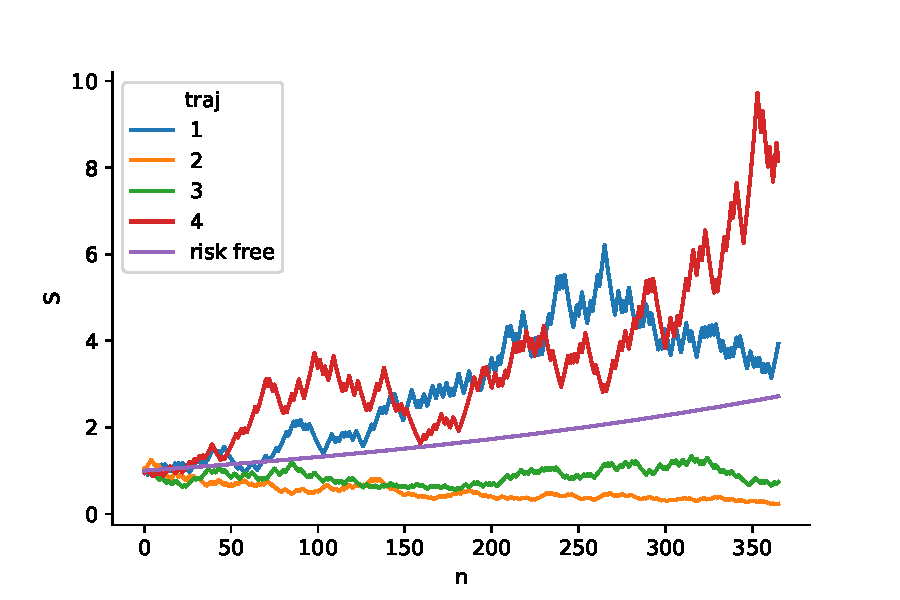
\includegraphics[width = \textwidth]{../Figures/traj_CRR.pdf}
\caption{Trajectoires du processus $S$ et de l'actif sans risque}
\label{fig:traj_CRR}
\end{figure}

Par analogie avec le modèle binomial, sous la probabilité risque neutre $\Q$, le processus $\tilde{S}_n = S_n/R_N^n,\text{ }n\geq0$ est une $\Q-$martingale. Les variables aléatoires $S_n$ sont mesurable par rapport à la tribu engendrée par les $\xi_i,\text{ }i\leq n$, noté $\mathcal{F}_n = \sigma_N(\xi_1,\ldots, \xi_n)$. La suite $(\F_n)_{n\geq0}$ est une suite de sous-tribu croissante pour l'inclusion que l'on appelle filtration du processus $S$. Il s'agit de l'information détenue sur le processus jusqu'à l'instant $n$. Le processus $\tilde S$ est une $\Q$-martingale s'il vérifie 
$$
\E_\Q(\tilde{S}_n|\F_{n-1}) =  \tilde S_{n-1}.
$$
On observe que 
\begin{eqnarray*}
\E_\Q(\tilde{S}_n|\F_{n-1})& =& \E_\Q\left[\frac{S_{n-1}}{R_N^n}\e^{\mu_N + \xi_{n}\sigma_N}|\F_{n-1}\right]\\
& =& \frac{S_{n-1}}{R_N^n}\e^\mu_N\E_\Q\left[\e^{\xi_{n}\sigma_N}|\F_{n-1}\right]\\
& =& \tilde S_{n-1}\frac{\e^\mu_N}{R_N}\E_\Q\left[\e^{\xi_{n}\sigma_N}\right]\\
& =& \tilde S_{n-1}\frac{q\e^{\mu_N+\sigma_N}+ (1-q)\e^{\mu_N-\sigma_N} }{R_N}\\
\end{eqnarray*}
Pour que $S$ soit une martingale, il faut que 
$$
q\e^{\mu_N+\sigma_N}+ (1-q)\e^{\mu_N-\sigma_N} = R_N \Leftrightarrow q = \frac{R_N-\e^{\mu-\sigma_N}}{\e^{\mu+\sigma_N}-\e^{\mu_N-\sigma_N}}.
$$
On a bien identifié la probabilité risque neutre $\Q$ telle que 
$$
\Q(\xi = 1) = \frac{R-e^{\mu_N-\sigma_N}}{\e^{\mu_N+\sigma_N}-\e^{\mu_N-\sigma_N}}=\frac{R_N-d_N}{u_N-d_N}=q_N
$$
de manière analogue au modèle binomial. La valorisation d'un produit dérivé $g(S_n)$ se fait sous la probabilité risque neutre avec 
$$
\pi = e^{-rT}\mathbb{E}_\Q[g(S_N)].
$$ 
Cette espérance se calcule bien en remarquant que 
$$
\Q\left(S_N = S_0u_N^kd_N^{N-k}\right) = \binom{N}{k}q_N^k(1-q_N)^{N-k},\text{ pour }k = 0,\ldots, N.
$$
Prenons l'exemple du call européen avec $g(s) = (s-K)_+$. Soit 
\begin{equation}\label{eq:eta}
\eta_N =\inf\{k = 0,\ldots, N\text{ ; }S_0u_N^kd_N^{N-k}>K\},
\end{equation}
et $\bar{F}(n,p,k) = \Prob[\BinomialDist(n,p)> k]
$. On a 
\begin{equation}\label{eq:price_call_Binomial}
\pi_N = R_N^{-N}\mathbb{E}_\Q[(S_N-K)_+] = S_0\bar{F}(N,\frac{q_Nu_N}{R_N},\eta_N)- e^{-rT}K \bar{F}(N,q_N,\eta_N).
\end{equation}
Le modèle de Cox-Ross-Rubinstein est une approximation d'un modèle en temps continu obtenu en laissant $N$ tendre vers l'infini. On note que sous la probabilité historique $\Prob$ et avec $p=1/2$, il vient
$$
\log\left(\frac{S_N}{S_0}\right) = N\mu_N+Z_N\sigma_N = \mu T + \frac{Z_N}{\sqrt{N}}\sigma\sqrt{T}\overset{\text{TCL}}{\sim}\NormalDist(\mu T, \sigma^2T)
$$
Les log rendements gaussien sont une caractéristique du modèle de Black-Scholes qu'on étudiera par la suite. Faire tendre $N$ vers l'infini permet également d'approcher le prix du call $\eqref{eq:price_call_Binomial}$. On a besoin du résultat suivant. 

\begin{lemma}
Soit $(X_n)_{n\geq0}$ une suite de \va indépendantes tel que $X_k\sim\BinomialDist(k, p_k)$ pour $k\geq1$ t alors 
$$
\frac{X_n-np_n}{\sqrt{np_n(1-p_n)}}\overset{\mathcal{D}}{\rightarrow}\NormalDist(0,1), \text{ lorsque }n\rightarrow\infty
$$
\end{lemma}
\begin{proof}
On montre que 
$$
\underset{n\rightarrow \infty}{\lim} \E(e^{tX_n})= \e^{t^2/2}.
$$
\end{proof}
D'après la définition de $\eta_N$, voir \eqref{eq:eta}, on a l'encadrement
$$
S_0u_N^{\eta_n-1}d_N^{N-\eta_n+1}\leq K\leq S_0u_N^{\eta_n}d_N^{N-\eta_n}.
$$
On en déduit en passant au log que  
$$
\eta_N\sigma\frac{\sqrt{T}}{\sqrt{N}} + N\left(\mu\frac{T}{N} - \sigma\frac{\sqrt{T}}{\sqrt{N}}\right) =\ln(K/S_0)+o(\sqrt{N})
$$
puis
$$
\eta_N = \frac{N}{2}+\frac{\sqrt{N}}{2\sigma\sqrt{T}}\left[\log(K/S_0)-\mu T\right]+ o(\sqrt{N})\text{, lorsque }N\rightarrow\infty.
$$
On a également
$$
q_{N} = \frac{e^{r\frac TN}-e^{\mu\frac TN-\sigma\sqrt{\frac{T}{N}}}}{e^{\mu\frac TN+\sigma\sqrt{\frac TN}} - e^{\mu\frac TN-\sigma\sqrt{\frac{T}{N}}}}
$$
Un développement limité à l'ordre 1 permet de conclure que $q_N\rightarrow 1/2$ pour $N\rightarrow +\infty$. Un développement limité à l'ordre 2 permet d'observer que 
$$
Nq_N = \frac{N}{2}+\frac{(r-\mu-\sigma^2/2)T}{2\sigma\sqrt{T}}\sqrt{N} + o(\sqrt{N})
$$
et de conclure que 
$$
\frac{\eta_N - Nq_N}{\sqrt{Nq_N(1-q_N)}} \rightarrow \frac{1}{\sigma\sqrt{T}}\left[\log(\widetilde{K}/S_0) + \sigma^2/2\right]= d^+,
$$
où $\widetilde{K} = Ke^{-rT}$. On a également 
$$
\frac{q_Nu_N}{R_N} = \frac{e^{r\frac TN}-e^{\mu\frac TN-\sigma\sqrt{\frac{T}{N}}}}{e^{\mu\frac TN+\sigma\sqrt{\frac TN}} - e^{\mu\frac TN-\sigma\sqrt{\frac{T}{N}}}}
\cdot 
\frac{e^{\mu\frac TN+\sigma\sqrt{\frac{T}{N}}}}{e^{r\frac TN}} = 
\frac{e^{(r+\mu)\frac TN+\sigma\sqrt{\frac TN}}-e^{2\mu\frac TN}}{e^{(r+\mu)\frac TN+\sigma\sqrt{\frac TN}} - e^{(r+\mu)\frac TN-\sigma\sqrt{\frac{T}{N}}}}
$$
Ce qui permet d'affirmer que 
$$\frac{q_Nu_N}{R_N}\rightarrow 1/2\text{, et }
N\frac{q_Nu_N}{R_N} = \frac{N}{2}+\frac{(r-\mu+\sigma^2/2)T}{2\sigma\sqrt{T}}\sqrt{N} + o(\sqrt{N})\text{ lorsque } N\rightarrow +\infty.
$$
Il vient alors 
$$
\frac{\eta_N - Nq_Nu_N/R_N}{\sqrt{Nq_Nu_N/R_N(1-q_Nu_N/R_N)}} \rightarrow \frac{1}{\sigma\sqrt{T}}\left[\log(\widetilde{K}/S_0) - \sigma^2/2\right] = d^-. 
$$
On conclut que 
$$
\pi_N\approx S_0[1-\phi(d^-)]- \widetilde{K} [1-\phi(d^+)].
$$
où $\phi(\cdot)$ est la fonction de répartition de la loi normal centrée réduite. On vérifie avec Python!
\section{Le modèle de Black-Scholes-(Merton)}\label{sec:BS}
\subsection{Le Set up}
Soit une économie comprenant deux actifs l'un risqué, l'autre non. Le prix de l'actif risqué (action ou indice boursier) est un processus $S$ défini sur un espace probabilisé filtré $(\Omega,\F, \F_t, \Prob)$ dont la dynamique est donnée 
par 
$$
\text{d}S_t = \mu \text{d}t + \sigma \text{d}B_t,
$$ 
où $(B_t)_{t\geq 0}$ est un mouvement brownien standard indépendant de $S_0$ la position initiale de $X$. Par application de la formule d'Ito sur $\ln S_t$, nous obtenons 
$$
S_t = S_0\exp[(\mu - \sigma^2/2)t + \sigma B_t],\text{ }t\geq 0.
$$
De son côté l'actif sans risque (bond du trésor américain ou livret A) admet une dynamique déterministe avec 
$$
\di S_t^0 = r S_t^0 \di t.
$$
où $r>0$ désigne le rendement de l'actif sans risque. En supposant que $S^0_0 = 1$, il vient 
$$
S_t^0 = \e^{r t}. 
$$
Un portefeuille contient contient à l'instant $t\geq 0$ une certaine part d'actif risqué et d'actif non-risqué. Soit $(a_t)_{t\geq 0}$ et $(b_t)_{t\geq 0}$ deux processus $\F_t$-adapté égale au nombre d'unité d'actif risqué et d'actif sans risque contenu dans le portefeuille. La valeur du portefeuille est donnée par 
$$
V_t = a_t S_t + b_t S^0_t,\text{ }t\geq 0.
$$
le couple $(a_t, b_t)_{t\geq 0}$ est une stratégie d'investissement. Nous supposons que la stratégie d'investissment est \textit{auto-finançante}, c'est à dire que les fluctuations de la valeur du portefeuille ne sont dues qu'aux fluctuations des prix des actifs. Cette hypothèse se traduit par 
$$
\di V_t = a_t \di S_t + b_t \di S^0_t = (a_t\mu S_t + b_tr S_t^0)\di t  + a_t \sigma S_t \di B_t.
$$
Nous souhaitons donner un prix juste à une option européenne de maturité $T$ et de prix d'exercice $K$. Selon Black, Scholes and Merton, la valeur juste est défini par deux hypothèses
\begin{itemize}
    \item L'existence d'une stratégie autofinançante permettant la réplication exacte du \textit{pay-off} de l'option. 
    \item Si l'option était vendu à un prix autre que le prix juste alors il y aurait une opportunité d'arbitrage, soit La possibilité d'un profit infini sans aucune prise de risque.
\end{itemize}
\subsection{La formule de Black-Scholes}
Prenons l'exemple d'un call européen pour lequel la \textit{pay-off} à maturité est donné par 
$$
(S_T-K)_+.
$$
L'objectif est de déterminer une stratégie autofinançante telle que 
$$
V_t = a_t S_t + b_t S^0_t = u(T-t, S_t),\text{ }t\in [0, T],
$$
où $u(\cdot, \cdot)$ est une fonction régulière qui vérifie la condition terminale 
$$
V_T = u(0,S_T) = (S_T-K)_+.
$$
On applique la formule d'Ito pour obtenir 
$$
\text{d}V_t = \left[-\frac{\partial}{\partial t}u(T-t, S_t) + \mu S_t\frac{\partial}{\partial x}u(T-t, S_t) + \frac{\sigma^2 S_t^2}{2}\frac{\partial^2}{\partial x^2}u(T-t, S_t)\right]\text{d}t + \sigma S_t\frac{\partial}{\partial x}u(T-t, S_t)\text{d}B_t.
$$
On se rappelle que du fait du caractère auto-finançant de la stratégie d'investissement alors
$$
\di V_t = (a_t\mu S_t + b_tr S_t^0)\di t  + a_t \sigma S_t \di B_t.
$$
De plus comme $V_t = a_t S_t + b_t S^0_t$ alors 
$$
b_t = \frac{V_t - a_t S_t}{S^0_t}
$$
et 
$$
\di V_t = (a_t(\mu - r)S_t + V_t r )\di t  + a_t \sigma S_t \di B_t.
$$
On en déduit que 
$$
a_t = \frac{\partial}{\partial x}u(T-t, S_t),
$$
et 
\begin{equation*}
\frac{\partial}{\partial x}u(T-t, S_t)(\mu - r)S_t + r u(T-t, S_t) = -\frac{\partial}{\partial t}u(T-t, S_t) + \mu S_t\frac{\partial}{\partial x}u(T-t, S_t) + \frac{\sigma^2 S_t^2}{2}\frac{\partial^2}{\partial x^2}u(T-t, S_t)
\end{equation*}
Cette dernière égalité est en fait une équation aux dérivées partielles
\begin{equation}\label{eq:edp_BS}
\frac{\partial}{\partial x}u(t, x)(\mu - r)x + r u(t, x) = -\frac{\partial}{\partial t}u(t, x) + \mu x\frac{\partial}{\partial x}u(t, x) + \frac{\sigma^2 x^2}{2}\frac{\partial^2}{\partial x^2}u(t, x),
\end{equation}
vérifiée pour $x>0$ et $t\in[0,T]$, avec la condition terminale 
$$
u(0,x) = (x-K)_+.
$$
L'équation \eqref{eq:edp_BS} admet une solution explicite (quelle chance). En effet, 
$$
u(t,x) = x\phi(g(t,x)) - K\e^{-rt}\phi(h(t,x)),
$$
où $\phi$ est la fonction de répartition de la loi normale centrée réduite, 
$$
g(t,x) = \frac{\log(x/K) + (r+\sigma^2/2)t}{\sigma \sqrt{t}},
$$
et 
$$
h(t,x) = g(t,x) - \sigma\sqrt{t}.
$$
Le prix juste pour notre option européenne est donnée par 
$$
V_0 = u(T, X_0) = X_0\phi(g(T,X_0)) - K\e^{-rt}\phi(h(T,X_0)).
$$
C'est la formule que l'on retrouve dans les papiers de \citet{Black1973} et \citet{Merton1973}. La stratégie d'investissemnt permettant la réplication du \textit{pay-off} st donnée par 
$$
a_t = \frac{\partial}{\partial x}u(T-t, S_t),
$$
et 
$$
b_t = \frac{u(T-t, X_t) - a_t X_t}{S^0_t}.
$$
Pour comprendre la signification du prix juste $q = u(T, X_0)$ en terme d'arbitrage, supposons que l'option soit vendu au prix $p>q$. On applique la stratégie suivante: à $t=0$
\begin{itemize}
    \item Je vends l'option au prix $p$, 
    \item J'investis $q$ dans la stratégie auto-finançante
\end{itemize}
Je dégage un profit initial $p-q$. A maturité si $X_T> K$ alors l'acheteur exerce l'option et ma stratégie autofinançante compense la perte $X_T-K$, sinon l'acheteur n'exerce pas l'option. Je peux dégagé un profit arbitrairement grand en supposant en vendant une grande quantité d'options.
\subsection{Interprétation via la probabilité risque-neutre}
Nous donnons une intéprétation du juste prix du call européen dans le cadre du modèle de Black-Scholes via un changement de mesure et le théorème de Girsanov. Un prix de départ raisonable est la valeur du flux de trésorie future actualisé au taux de l'actif sans risque soit
$$
\e^{-rT}(X_T - K)_+ = \e^{-rT}h(S_T)
$$
Le prix juste ne correspond pas à l'espérance du flux futur actualisé en tout cas pas sous la probabilité $\Prob$ dite historique. Il faut introduire une autre probalité dite risque neutre $\Q$. Dans la section précédente, cette probabilité était telle que le prix de l'actif actualisé était une martingale. Nous devons donc définir une probabilité pour laquelle le processus 
$$
\tilde{S}_t = \e^{-rt}S_t,\text{ }t\geq 0,
$$
est une $\Q$-martingale. Par application de la formule d'Ito, il vient 
$$
\text{d}\tilde{S}_t = \tilde{S}_t (\mu- r)\text{d}t + \tilde{S}_t \sigma\text{d}B_t.
$$
On définit $\tilde{B}_t = B_t - \frac{\mu - r}{\sigma}t,\text{ }t\geq0$. D'après le théorème de Girsanov $(\tilde{B}_t)_{t\geq 0}$ est un mouvement brownien sous la probabilité $\Q$ définie par 
$$
\Q(A) = \E_\Prob(Z_T^\theta\ind_A),
$$
où $Z_T^\theta = \e^{\theta B_t  - \theta t}$, et $\theta = \frac{\mu - r}{\sigma}.$ Le processus $(\tilde{S}_t)_{t\geq 0}$ dont la dynamique est donnée par 
$$
\text{d}\tilde{S}_t = \sigma\tilde{S}_t\text{d}\tilde{B}_t,
$$
est une $\Q$-martingale. Si on suppose qu'il existe une stratégie auto-finançante telle que 
$$
V_t = a_t S_t + b_t\beta_t
$$
tel que $V_T = h(S_T)$ alors la valeur du portefeuille à $T$ actualisée au temps $t$ est donnée par 
$$
\E(\e^{-r(T-t)}h(S_T)|\F_t),\text{ }t\in [0,T].
$$
Soit 
$$
\tilde{V_t} = \e^{-rt}V_t,\text{ }t\geq 0,
$$
la valeur actualisé du portefeuille. Par application de la formule d'Ito, il vient 
\begin{eqnarray*}
\text{d}\tilde{V_t}  &=& -r\e^{-rt}V_t\text{d}t + \e^{-rt}\text{d}V_t\\
 &=&-r\e^{-rt}(a_t S_t + b_tS_t^0)\text{d}t + \e^{-rt}(a_t S_t + b_tS_t^0 ))\\
 &=&a_t(-r\e^{-rt}S_t\text{d}t + \e^{-rt}\text{d}S_t)\\
 &=&a_t\text{d}\tilde{S}_t
\end{eqnarray*}
Le processus est une $\Q$-martingale et donc 
$$
V_t = \E^\Q(\tilde{V}_T|\F_t),\text{ }t\in [0,T].
$$
On en déduit que 
$$
V_t = \E^\Q(\e^{-r(T-t)}h(X_T)|\F_t),\text{ }t\in [0,T].
$$
La dynamique de $(X_t)_{t\geq 0}$ est donnée par 
$$
\di X_t = r \di t + \sigma\di  \tilde{B}_t,
$$
et donc 
$$
X_t = X_0 \e^{(r-\sigma^2 / 2)t + \sigma \tilde{B}_t }.
$$

On a alors 
$$
V_t = f(t, X_t) = \E^\Q\left[\e^{-r(T-t)}h(X_t\e^{(r-\sigma^2 / 2)(T)-t + \sigma (\tilde{B}_T - \tilde{B}_t})|\F_t\right],
$$
qui est l'espérance d'une fonction d'une variable aléatoire $\NormalDist(0,T-t)$. On vérifie par le calcul intégrale que l'on retrouve l'expression du prix juste de l'option avec $V_0$





\newpage




\end{document}


